% Laporan UAS Business Intelligence Systems - KIRANA. Kompilasi: cd laporan_akhir && latexmk -pdf UAS_BI_24120500031_TitanioYudista_Laporan.tex
% Ubah identitas di dua baris berikut. Seluruh isi laporan ada di berkas ini (cari penanda '% ======== ' untuk tiap dokumen).
\newcommand{\nama}{Titanio Yudista}
\newcommand{\nim}{24120500031}

\documentclass[10pt,a4paper]{article}
\usepackage[margin=13mm,bottom=16mm]{geometry}
\usepackage[utf8]{inputenc}\usepackage[T1]{fontenc}
\usepackage{newunicodechar}
\newunicodechar{−}{\ensuremath{-}}\newunicodechar{→}{\ensuremath{\rightarrow}}\newunicodechar{≤}{\ensuremath{\leq}}\newunicodechar{≥}{\ensuremath{\geq}}
\newunicodechar{≈}{\ensuremath{\approx}}\newunicodechar{≠}{\ensuremath{\neq}}\newunicodechar{±}{\ensuremath{\pm}}\newunicodechar{·}{\ensuremath{\cdot}}
\usepackage{lmodern}\usepackage[scaled=0.95]{helvet}\renewcommand{\familydefault}{\sfdefault}
\usepackage{longtable,booktabs,array,calc,graphicx,xcolor,etoolbox,pdfpages,fancyhdr,caption,float}
\floatplacement{figure}{H}\renewcommand{\figurename}{Gambar}
\usepackage[colorlinks=true,urlcolor=aksen,linkcolor=black]{hyperref}
\newcommand{\gh}[1]{\href{https://github.com/titan2903/kirana-omnichannel-performance-intelligence/blob/master/#1}{#1}}  % tautan file repo di dalam blok perintah (Verbatim)
\usepackage{xurl}\newcounter{none}\usepackage{fvextra}\DefineVerbatimEnvironment{verbatim}{Verbatim}{breaklines,fontsize=\scriptsize}
\usepackage[normalem]{ulem}
\definecolor{aksen}{HTML}{2A78D6}
\providecommand{\tightlist}{\setlength{\itemsep}{1pt}\setlength{\parskip}{0pt}}
\providecommand{\pandocbounded}[1]{\begin{center}\includegraphics[width=\linewidth]{#1}\end{center}}
\renewcommand{\pandocbounded}[1]{\resizebox{\linewidth}{!}{#1}}
\AtBeginEnvironment{longtable}{\scriptsize\setlength{\tabcolsep}{3pt}\renewcommand{\arraystretch}{1.15}}
\setlength{\parindent}{0pt}\setlength{\parskip}{4pt}\setlength{\emergencystretch}{3em}\sloppy
\setcounter{secnumdepth}{0}\setcounter{tocdepth}{1}
\usepackage{titlesec}
\titleformat{\section}{\Large\bfseries}{}{0pt}{}[{\color{aksen}\titlerule[1.2pt]}]
\titlespacing*{\section}{0pt}{14pt}{6pt}
\titleformat{\subsection}{\large\bfseries}{}{0pt}{}\titleformat{\subsubsection}{\normalsize\bfseries}{}{0pt}{}
\pagestyle{fancy}\fancyhf{}\fancyfoot[C]{\scriptsize UAS BI KIRANA -- \thepage}\renewcommand{\headrulewidth}{0pt}

% judul bagian dimulai di halaman baru dan masuk daftar isi
\newcommand{\bagian}[1]{\clearpage\phantomsection\addcontentsline{toc}{section}{#1}%
  {\centering\LARGE\bfseries\color{aksen} #1\par}\vspace{6pt}}

\begin{document}\small
\begin{titlepage}
\vspace*{25mm}
{\fontsize{26}{30}\selectfont\bfseries KIRANA Omnichannel\\Performance Intelligence\par}
\vspace{6mm}{\large\color{gray} Laporan UAS Business Intelligence Systems\\Universitas Cakrawala, Sains Data, Blok A\par}
\vspace{10mm}
\begin{tabular}{@{}ll@{}}
\textbf{Nama} & \nama\\ \textbf{NIM} & \nim\\ \textbf{Periode data} & 1 Jan 2024 -- 30 Jun 2026\\
\textbf{Keputusan} & Realokasi anggaran promo dan program perbaikan toko/region, H2 2026
\end{tabular}
\vspace{6mm}\par\textbf{Daftar isi}\par\renewcommand{\contentsname}{}\tableofcontents
\end{titlepage}
\setcounter{page}{2}

\bagian{Bagian A. Dokumentasi teknis}
% ======== A1_decision_statement ========
\section{A1. Decision Statement}\label{a1.-decision-statement}

\subsection{Pernyataan keputusan}\label{pernyataan-keputusan}

\begin{quote}
\textbf{Pada awal Juli 2026, Direktur Komersial KIRANA Home \& Living memutuskan, untuk periode H2 2026:}
\textbf{(1)} bagaimana anggaran promo direalokasikan antar-channel (Store, Website, Mobile App, Marketplace),
antar-kategori produk, dan antar-mekanisme promo; dan
\textbf{(2)} toko atau region mana yang masuk program perbaikan kinerja.
Keputusan memakai data 1 Januari 2024 -- 30 Juni 2026 dari satu sumber angka yang disepakati
Commercial dan Finance.
\end{quote}

{\def\LTcaptype{none} % do not increment counter
\begin{longtable}[]{@{}
  >{\raggedright\arraybackslash}p{(\linewidth - 2\tabcolsep) * \real{0.3200}}
  >{\raggedright\arraybackslash}p{(\linewidth - 2\tabcolsep) * \real{0.6800}}@{}}
\toprule\noalign{}
\begin{minipage}[b]{\linewidth}\raggedright
Unsur
\end{minipage} & \begin{minipage}[b]{\linewidth}\raggedright
Isi
\end{minipage} \\
\midrule\noalign{}
\endhead
\bottomrule\noalign{}
\endlastfoot
\textbf{Keputusan 1} & Realokasi anggaran promo (channel, kategori, mekanisme: Ramadan, Clearance, Member Day, App Payday, Mega Sale, Harbolnas) \\
\textbf{Keputusan 2} & Pemilihan toko/region untuk program perbaikan kinerja H2 2026 \\
\textbf{Pengambil keputusan} & Direktur Komersial \\
\textbf{Waktu keputusan} & Awal Juli 2026 (rapat keputusan H2 2026); batas data 30 Juni 2026 \\
\textbf{Peran analis} & BI Analyst / Analytics Engineer, tim Data \& Analytics \\
\end{longtable}
}

\subsection{Pemangku kepentingan}\label{pemangku-kepentingan}

{\def\LTcaptype{none} % do not increment counter
\begin{longtable}[]{@{}
  >{\raggedright\arraybackslash}p{(\linewidth - 4\tabcolsep) * \real{0.2100}}
  >{\raggedright\arraybackslash}p{(\linewidth - 4\tabcolsep) * \real{0.3700}}
  >{\raggedright\arraybackslash}p{(\linewidth - 4\tabcolsep) * \real{0.4200}}@{}}
\toprule\noalign{}
\begin{minipage}[b]{\linewidth}\raggedright
Pemangku kepentingan
\end{minipage} & \begin{minipage}[b]{\linewidth}\raggedright
Kepentingan terhadap keputusan
\end{minipage} & \begin{minipage}[b]{\linewidth}\raggedright
Yang dibutuhkan dari BI
\end{minipage} \\
\midrule\noalign{}
\endhead
\bottomrule\noalign{}
\endlastfoot
Direktur Komersial (utama) & Memutuskan keputusan 1 dan 2 & Satu angka yang dapat dipercaya, rekomendasi dengan dampak dan risiko \\
Head of Store Operations & Keputusan 2 (toko/region), kejadian operasional toko & Pembeda masalah bisnis (renovasi, tren) dan masalah data (sync gagal) \\
Head of E-Commerce & Keputusan 1 untuk Website, Mobile App, Marketplace & Efektivitas promo online, dampak komisi Marketplace, retur online \\
Finance Controller & Validasi angka sales, margin, HPP, biaya channel & Definisi metrik tertulis, rekonsiliasi dari raw ke angka laporan \\
\end{longtable}
}

\subsection{Ukuran keputusan}\label{ukuran-keputusan}

\begin{itemize}
\tightlist
\item
  \textbf{Keputusan 1:} promo lift terhadap baseline, dampak ke gross margin dan contribution margin (setelah biaya channel), serta pemakaian anggaran terhadap \texttt{budget\_\allowbreak{}idr} per promo.
\item
  \textbf{Keputusan 2:} pencapaian terhadap target (region), tren dan kontribusi toko, dengan kriteria tegas yang memisahkan toko bermasalah karena bisnis dari toko yang datanya tidak lengkap.
\end{itemize}

\subsection{Pemetaan pertanyaan bisnis ke keputusan}\label{pemetaan-pertanyaan-bisnis-ke-keputusan}

{\def\LTcaptype{none} % do not increment counter
\begin{longtable}[]{@{}
  >{\raggedright\arraybackslash}p{(\linewidth - 8\tabcolsep) * \real{0.0404}}
  >{\raggedright\arraybackslash}p{(\linewidth - 8\tabcolsep) * \real{0.3333}}
  >{\raggedright\arraybackslash}p{(\linewidth - 8\tabcolsep) * \real{0.0707}}
  >{\raggedright\arraybackslash}p{(\linewidth - 8\tabcolsep) * \real{0.2828}}
  >{\raggedright\arraybackslash}p{(\linewidth - 8\tabcolsep) * \real{0.2727}}@{}}
\toprule\noalign{}
\begin{minipage}[b]{\linewidth}\raggedright
\#
\end{minipage} & \begin{minipage}[b]{\linewidth}\raggedright
Pertanyaan bisnis
\end{minipage} & \begin{minipage}[b]{\linewidth}\raggedright
Keputusan
\end{minipage} & \begin{minipage}[b]{\linewidth}\raggedright
KPI utama
\end{minipage} & \begin{minipage}[b]{\linewidth}\raggedright
Tab dashboard
\end{minipage} \\
\midrule\noalign{}
\endhead
\bottomrule\noalign{}
\endlastfoot
1 & Pencapaian net sales FY2025 dan H1 2026 terhadap target per channel, region, toko & 2 (dan 1) & Net Sales, Achievement vs Target \% & 1 Executive Overview; 2 Channel, Region \& Store \\
2 & Tren, musiman, dan pergeseran kontribusi antar-channel & 1 & Net Sales, kontribusi channel \% & 1 Executive Overview; 2 Channel, Region \& Store \\
3 & Kategori, channel, promo yang menekan gross margin dan contribution margin & 1 & Gross Margin \%, Contribution Margin \% & 3 Margin \& Promosi \\
4 & Efektivitas promo (Ramadan, Clearance, Member Day, App Payday, Mega Sale, Harbolnas) & 1 & Promo Lift, dampak margin promo & 3 Margin \& Promosi \\
5 & Toko berkinerja rendah dan penyebabnya (bisnis atau data) & 2 & Achievement \%, tren toko, flag data tidak lengkap & 2 Channel, Region \& Store \\
6 & Tingkat dan alasan retur per kategori dan channel & 1 dan 2 & Return Rate, distribusi alasan & 4 Retur \& Customer \\
7 & Aktivitas dan repeat purchase member per channel & 1 & Active Members, Repeat Rate & 4 Retur \& Customer \\
\end{longtable}
}

\subsection{Asumsi dan batas ruang lingkup}\label{asumsi-dan-batas-ruang-lingkup}

\begin{itemize}
\tightlist
\item
  Target tersedia hanya untuk FY2025 dan H1 2026 (tidak ada target 2024). Target Store ditetapkan per region, target online per channel nasional; tidak ada target per toko.
\item
  Nilai dalam Rupiah, tidak termasuk pajak.
\item
  Biaya di luar \texttt{channel\_\allowbreak{}fee\_\allowbreak{}rates.csv} (biaya operasional toko, biaya marketing di luar \texttt{promotions.budget\_\allowbreak{}idr}) tidak tersedia, sehingga contribution margin hanya dikurangi biaya channel.
\item
  Seluruh angka berasal dari model di \texttt{kirana.duckdb}; tidak ada data eksternal.
\end{itemize}

% ======== A2_profiling ========
\section{A2. Data Profiling}\label{a2.-data-profiling}

Profiling dilakukan langsung dari \texttt{raw\_\allowbreak{}data/} dengan DuckDB, tanpa mengubah file. Semua angka dapat
diulang dengan:

\begin{Verbatim}[commandchars=\\\{\},breaklines,fontsize=\scriptsize]
duckdb -markdown < \gh{sql/profiling/01_file_inventory.sql}   # inventaris, keunikan kunci, null per kolom
duckdb -markdown < \gh{sql/profiling/02_issue_impact.sql}     # dampak per isu, 53 pengecekan, kontrol sync log
duckdb -markdown < \gh{sql/profiling/03_distributions.sql}    # sebaran nilai dan statistik yang dikutip di bawah
\end{Verbatim}

Kode \texttt{DQ-xx} merujuk ke Data Quality Issue Log (A3).

\subsection{1. Inventaris file}\label{inventaris-file}

{\def\LTcaptype{none} % do not increment counter
\begin{longtable}[]{@{}
  >{\raggedright\arraybackslash}p{(\linewidth - 12\tabcolsep) * \real{0.1650}}
  >{\raggedright\arraybackslash}p{(\linewidth - 12\tabcolsep) * \real{0.1165}}
  >{\raggedleft\arraybackslash}p{(\linewidth - 12\tabcolsep) * \real{0.1068}}
  >{\raggedright\arraybackslash}p{(\linewidth - 12\tabcolsep) * \real{0.1553}}
  >{\raggedleft\arraybackslash}p{(\linewidth - 12\tabcolsep) * \real{0.0777}}
  >{\raggedright\arraybackslash}p{(\linewidth - 12\tabcolsep) * \real{0.1748}}
  >{\raggedright\arraybackslash}p{(\linewidth - 12\tabcolsep) * \real{0.2039}}@{}}
\toprule\noalign{}
\begin{minipage}[b]{\linewidth}\raggedright
File
\end{minipage} & \begin{minipage}[b]{\linewidth}\raggedright
Sumber
\end{minipage} & \begin{minipage}[b]{\linewidth}\raggedleft
Baris
\end{minipage} & \begin{minipage}[b]{\linewidth}\raggedright
Kolom kunci
\end{minipage} & \begin{minipage}[b]{\linewidth}\raggedleft
Kunci unik
\end{minipage} & \begin{minipage}[b]{\linewidth}\raggedright
Periode
\end{minipage} & \begin{minipage}[b]{\linewidth}\raggedright
Catatan
\end{minipage} \\
\midrule\noalign{}
\endhead
\bottomrule\noalign{}
\endlastfoot
\texttt{sales\_\allowbreak{}pos\_\allowbreak{}transactions.csv} & POS toko & 264.420 & \texttt{trx\_\allowbreak{}id}+\texttt{line\_\allowbreak{}no} & 262.823 & 2024-01-01 s.d. 2026-06-30 & 1.597 kunci ganda (DQ-04, DQ-05) \\
\texttt{sales\_\allowbreak{}online\_\allowbreak{}orders.csv} & Platform e-commerce & 209.626 & \texttt{order\_\allowbreak{}no}+\texttt{line\_\allowbreak{}no} & 209.394 & 2024-01-01 s.d. 2026-06-30 & 232 kunci ganda (DQ-10) \\
\texttt{products.csv} & Master produk & 606 & \texttt{sku} & 600 & launch 2021-07-17 s.d. 2025-11-24 & 6 SKU ganda (DQ-13) \\
\texttt{product\_\allowbreak{}cost\_\allowbreak{}history.csv} & Finance & 850 & \texttt{sku}+\texttt{valid\_\allowbreak{}from} & 850 & 2023-01-01 s.d. 9999-12-31 & 600 SKU; bersih \\
\texttt{stores.csv} & Master toko & 18 & \texttt{store\_\allowbreak{}code} & 18 & buka 2019-03-01 s.d. 2025-01-15 & Semua \texttt{Active} \\
\texttt{store\_\allowbreak{}region\_\allowbreak{}history.csv} & Store Operations & 2 & \texttt{store\_\allowbreak{}code}+\texttt{valid\_\allowbreak{}from} & 2 & 2021-08-01 s.d. 2025-07-01 & Hanya BGR-01 (DQ-15) \\
\texttt{store\_\allowbreak{}events.csv} & Store Operations & 1 & \texttt{store\_\allowbreak{}code}+\texttt{start\_\allowbreak{}date} & 1 & 2025-08-04 s.d. 2025-09-21 & Renovasi SBY-01 \\
\texttt{customers.csv} & CRM & 42.320 & \texttt{customer\_\allowbreak{}id} & 42.320 & join 2023-06-16 s.d. 2026-06-18 & Berisi PII \\
\texttt{returns.csv} & Customer Service & 18.090 & \texttt{return\_\allowbreak{}id} & 18.090 & 2024-01-03 s.d. 2026-06-30 & Refund total Rp 3.702.006.200 \\
\texttt{promotions.csv} & Marketing & 73 & \texttt{promo\_\allowbreak{}code} & 73 & 2024-01-05 s.d. 2026-06-28 & Diskon 10 s.d. 45\% \\
\texttt{channel\_\allowbreak{}fee\_\allowbreak{}rates.csv} & Finance & 5 & \texttt{channel}+\texttt{valid\_\allowbreak{}from} & 5 & 2024-01-01 s.d. 2099-12-31 & Marketplace 9,0\% → 11,5\% mulai 2025-04-01 \\
\texttt{pos\_\allowbreak{}sync\_\allowbreak{}log.csv} & IT & 16.036 & \texttt{store\_\allowbreak{}code}+\texttt{business\_\allowbreak{}date} & 16.036 & 2024-01-01 s.d. 2026-06-30 & 15.980 SUCCESS, 49 STORE\_\allowbreak{}CLOSED, 7 FAILED \\
\texttt{sales\_\allowbreak{}targets\_\allowbreak{}2025\_\allowbreak{}2026.xlsx} & FP\&A & 9 + 9 + 4 baris & \texttt{channel}+\texttt{region} & 9 / 9 / 4 & FY2025, H1 2026 & 3 sheet; header di baris 3 (DQ-16) \\
\end{longtable}
}

Cakupan sync log: 16.036 toko-hari, sama dengan 18 toko x 912 hari dikurangi 380 hari DPS-01 sebelum
dibuka (2025-01-15).

\subsection{2. Kolom dengan nilai kosong}\label{kolom-dengan-nilai-kosong}

{\def\LTcaptype{none} % do not increment counter
\begin{longtable}[]{@{}
  >{\raggedright\arraybackslash}p{(\linewidth - 8\tabcolsep) * \real{0.2941}}
  >{\raggedright\arraybackslash}p{(\linewidth - 8\tabcolsep) * \real{0.1765}}
  >{\raggedleft\arraybackslash}p{(\linewidth - 8\tabcolsep) * \real{0.1078}}
  >{\raggedleft\arraybackslash}p{(\linewidth - 8\tabcolsep) * \real{0.0882}}
  >{\raggedright\arraybackslash}p{(\linewidth - 8\tabcolsep) * \real{0.3333}}@{}}
\toprule\noalign{}
\begin{minipage}[b]{\linewidth}\raggedright
File
\end{minipage} & \begin{minipage}[b]{\linewidth}\raggedright
Kolom
\end{minipage} & \begin{minipage}[b]{\linewidth}\raggedleft
Kosong
\end{minipage} & \begin{minipage}[b]{\linewidth}\raggedleft
\%
\end{minipage} & \begin{minipage}[b]{\linewidth}\raggedright
Penjelasan
\end{minipage} \\
\midrule\noalign{}
\endhead
\bottomrule\noalign{}
\endlastfoot
\texttt{sales\_\allowbreak{}pos\_\allowbreak{}transactions.csv} & \texttt{promo\_\allowbreak{}code} & 238.872 & 90,34 & Wajar: tanpa promo \\
\texttt{sales\_\allowbreak{}pos\_\allowbreak{}transactions.csv} & \texttt{member\_\allowbreak{}id} & 118.995 & 45,00 & Wajar: bukan member \\
\texttt{sales\_\allowbreak{}online\_\allowbreak{}orders.csv} & \texttt{voucher\_\allowbreak{}code} & 180.705 & 86,20 & Wajar: tanpa voucher \\
\texttt{sales\_\allowbreak{}online\_\allowbreak{}orders.csv} & \texttt{ship\_\allowbreak{}province} & 2.109 & 1,01 & \textbf{Masalah data} (DQ-12) \\
\texttt{returns.csv} & \texttt{store\_\allowbreak{}code} & 12.289 & 67,93 & Wajar: seluruhnya retur online \\
\texttt{pos\_\allowbreak{}sync\_\allowbreak{}log.csv} & \texttt{synced\_\allowbreak{}at} & 56 & 0,35 & Wajar: 49 STORE\_\allowbreak{}CLOSED + 7 FAILED \\
\end{longtable}
}

Kolom lain pada file di atas, serta \texttt{products}, \texttt{stores}, dan \texttt{customers}, tidak memiliki nilai kosong.

\subsection{3. Profiling per sumber}\label{profiling-per-sumber}

\subsubsection{\texorpdfstring{3.1 POS (\texttt{sales\_\allowbreak{}pos\_\allowbreak{}transactions.csv})}{3.1 POS (sales\_\allowbreak{}pos\_\allowbreak{}transactions.csv)}}\label{pos-sales_pos_transactions.csv}

{\def\LTcaptype{none} % do not increment counter
\begin{longtable}[]{@{}
  >{\raggedright\arraybackslash}p{(\linewidth - 2\tabcolsep) * \real{0.2800}}
  >{\raggedright\arraybackslash}p{(\linewidth - 2\tabcolsep) * \real{0.7200}}@{}}
\toprule\noalign{}
\begin{minipage}[b]{\linewidth}\raggedright
Aspek
\end{minipage} & \begin{minipage}[b]{\linewidth}\raggedright
Hasil
\end{minipage} \\
\midrule\noalign{}
\endhead
\bottomrule\noalign{}
\endlastfoot
Format tanggal & 100\% \texttt{YYYY-MM-DD\ HH:MM:SS}, semua dalam periode \\
Harga dan diskon & \texttt{unit\_\allowbreak{}price} \textgreater{} 0 pada semua baris; diskon tidak pernah melebihi nilai kotor \\
\texttt{qty} & 262.320 baris 1--3 unit, 2.086 baris negatif (void kasir), 14 baris 152--446 unit (B2B bulk, DQ-07) \\
\texttt{store\_\allowbreak{}code} & 38 kode untuk 18 toko: 3.236 baris huruf kecil (DQ-01); \texttt{TRN-99} 324 baris tidak ada di master (DQ-02) \\
\texttt{sku} & 2.650 baris berspasi/huruf kecil (DQ-03); setelah normalisasi 600 SKU, semuanya ada di \texttt{products} \\
Member & 145.425 baris (55,0\%) berisi \texttt{member\_\allowbreak{}id}; semuanya ada di \texttt{customers} \\
Duplikat kunci & 1.597 grup: 1.577 salinan persis (DQ-04) dan 20 tabrakan nomor struk (DQ-05) \\
Void & 2.068 baris void (setelah dedup), 2.067 terpasang ke baris asli (DQ-06) \\
Promo & Semua \texttt{promo\_\allowbreak{}code} ada di \texttt{promotions}, kecuali \texttt{B2B-CORP} (14 baris, DQ-07) \\
Transaksi distinct & 144.089 \texttt{trx\_\allowbreak{}id} (sebelum pembersihan) \\
Metode bayar & QRIS 79.404; Debit 79.151; Cash 52.970; Credit Card 52.895 \\
\end{longtable}
}

\subsubsection{\texorpdfstring{3.2 Online (\texttt{sales\_\allowbreak{}online\_\allowbreak{}orders.csv})}{3.2 Online (sales\_\allowbreak{}online\_\allowbreak{}orders.csv)}}\label{online-sales_online_orders.csv}

{\def\LTcaptype{none} % do not increment counter
\begin{longtable}[]{@{}
  >{\raggedright\arraybackslash}p{(\linewidth - 2\tabcolsep) * \real{0.2500}}
  >{\raggedright\arraybackslash}p{(\linewidth - 2\tabcolsep) * \real{0.7500}}@{}}
\toprule\noalign{}
\begin{minipage}[b]{\linewidth}\raggedright
Aspek
\end{minipage} & \begin{minipage}[b]{\linewidth}\raggedright
Hasil
\end{minipage} \\
\midrule\noalign{}
\endhead
\bottomrule\noalign{}
\endlastfoot
Format tanggal & 100\% \texttt{DD/MM/YYYY\ HH:MM}, semua dalam periode; awalan \texttt{order\_\allowbreak{}no} (24/25/26) sesuai tahun order \\
\texttt{item\_\allowbreak{}price} & 173.447 baris angka polos; 36.179 baris berformat \texttt{Rp100.900} (DQ-09). Setelah parse, tidak ada harga gagal atau ≤ 0 \\
\texttt{sales\_\allowbreak{}channel} & 12 label untuk 3 channel (DQ-08); semuanya terpetakan, tidak ada order yang terpecah ke dua channel \\
\texttt{qty} & 157.039 baris 1 unit, 52.587 baris 2 unit; tidak ada ≤ 0 \\
Status & 196.881 COMPLETED, 12.745 CANCELLED (6,08\% baris) (DQ-11) \\
Voucher & Semua kode ada di \texttt{promotions}; voucher tidak pernah melebihi nilai kotor; kode dan nilai selalu berpasangan \\
Customer & Semua \texttt{customer\_\allowbreak{}id} ada di \texttt{customers} dan berformat \texttt{Mxxxxxx}; tidak ada order tanpa customer \\
\texttt{ship\_\allowbreak{}province} & 13 provinsi + 2.109 kosong (DQ-12). Sulawesi Selatan dan Kalimantan Timur berada di luar enam region → \texttt{Lainnya} \\
Duplikat kunci & 232 grup, semuanya salinan persis (DQ-10), tidak ada konflik nilai/status \\
Order distinct & 140.573 \texttt{order\_\allowbreak{}no} (sebelum pembersihan) \\
Metode bayar & E-Wallet 73.445; Virtual Account 63.194; COD 26.972; Credit Card 25.138; Paylater 20.877 \\
\end{longtable}
}

Harga transaksi POS dan online berada pada 94,8\%--100\% dari \texttt{current\_\allowbreak{}list\_\allowbreak{}price} (rata-rata 98,8\% POS,
99,0\% online). Itu menunjukkan harga jual berubah dari waktu ke waktu, bukan galat; analisis memakai
harga transaksi, bukan harga master.

\subsubsection{3.3 Master produk, HPP, toko}\label{master-produk-hpp-toko}

{\def\LTcaptype{none} % do not increment counter
\begin{longtable}[]{@{}
  >{\raggedright\arraybackslash}p{(\linewidth - 2\tabcolsep) * \real{0.3700}}
  >{\raggedright\arraybackslash}p{(\linewidth - 2\tabcolsep) * \real{0.6300}}@{}}
\toprule\noalign{}
\begin{minipage}[b]{\linewidth}\raggedright
Aspek
\end{minipage} & \begin{minipage}[b]{\linewidth}\raggedright
Hasil
\end{minipage} \\
\midrule\noalign{}
\endhead
\bottomrule\noalign{}
\endlastfoot
\texttt{products} & 606 baris, 600 SKU: 6 SKU ganda dengan varian nama \texttt{(old)} (DQ-13). Kategori punya 9 SKU berlabel \texttt{Home\ Décor} dan 5 SKU \texttt{kitchen\ \&\ dining} (DQ-14). Harga dan HPP \textgreater{} 0, HPP selalu di bawah harga \\
\texttt{product\_\allowbreak{}cost\_\allowbreak{}history} & 850 baris untuk 600 SKU. Tanpa overlap, tanpa celah, \texttt{valid\_\allowbreak{}from} ≤ \texttt{valid\_\allowbreak{}to}, HPP aktif sama dengan \texttt{products.current\_\allowbreak{}unit\_\allowbreak{}cost}. 350 SKU satu periode; 250 SKU dua periode, semuanya naik (rata-rata +7,4\%): 60 SKU berubah 2025-07-01 (rata-rata +18\%) dan 190 SKU berubah 2026-01-01 (rata-rata +4\%) \\
Penjualan sebelum \texttt{launch\_\allowbreak{}date} & 126 baris, Rp 27,8 juta, seluruhnya baris asli yang kemudian di-void (DQ-17, sudah tercakup DQ-06b). Penjualan valid sebelum launch: 0 \\
\texttt{stores} & 18 toko, 6 region, tipe Flagship/Regular/Express; tidak ada penjualan sebelum \texttt{open\_\allowbreak{}date} \\
\texttt{store\_\allowbreak{}region\_\allowbreak{}history} & Hanya BGR-01: Jawa Barat s.d. 2025-06-30, Jabodetabek mulai 2025-07-01 (DQ-15). Toko lain tidak punya riwayat \\
\texttt{channel\_\allowbreak{}fee\_\allowbreak{}rates} & Store 0,7\%; Website dan Mobile App 2,2\%; Marketplace 9,0\% s.d. 2025-03-31 lalu 11,5\% \\
\end{longtable}
}

\subsubsection{3.4 Customers (hanya agregat; tanpa nilai PII)}\label{customers-hanya-agregat-tanpa-nilai-pii}

{\def\LTcaptype{none} % do not increment counter
\begin{longtable}[]{@{}
  >{\raggedright\arraybackslash}p{(\linewidth - 2\tabcolsep) * \real{0.2700}}
  >{\raggedright\arraybackslash}p{(\linewidth - 2\tabcolsep) * \real{0.7300}}@{}}
\toprule\noalign{}
\begin{minipage}[b]{\linewidth}\raggedright
Aspek
\end{minipage} & \begin{minipage}[b]{\linewidth}\raggedright
Hasil
\end{minipage} \\
\midrule\noalign{}
\endhead
\bottomrule\noalign{}
\endlastfoot
Kunci & 42.320 \texttt{customer\_\allowbreak{}id} unik, tidak ada kolom kosong \\
Tier & Silver 29.741; Gold 10.026; Platinum 2.553 \\
\texttt{join\_\allowbreak{}channel} & Store 17.834; Marketplace 10.439; Mobile App 7.409; Website 6.638 \\
\texttt{birth\_\allowbreak{}date} & 418 bernilai sentinel 1900-01-01 (DQ-18); selain itu rentang sampai 2006 \\
Email ganda & 491 grup berisi 982 member (DQ-19). Nomor telepon: 320 baris memakai nomor yang sudah muncul sebelumnya \\
Tanpa transaksi & 2.753 member tidak pernah bertransaksi (DQ-20) \\
Konsistensi waktu & Tidak ada transaksi POS sebelum \texttt{join\_\allowbreak{}date} \\
\end{longtable}
}

\subsubsection{\texorpdfstring{3.5 Retur (\texttt{returns.csv})}{3.5 Retur (returns.csv)}}\label{retur-returns.csv}

{\def\LTcaptype{none} % do not increment counter
\begin{longtable}[]{@{}
  >{\raggedright\arraybackslash}p{(\linewidth - 2\tabcolsep) * \real{0.2000}}
  >{\raggedright\arraybackslash}p{(\linewidth - 2\tabcolsep) * \real{0.8000}}@{}}
\toprule\noalign{}
\begin{minipage}[b]{\linewidth}\raggedright
Aspek
\end{minipage} & \begin{minipage}[b]{\linewidth}\raggedright
Hasil
\end{minipage} \\
\midrule\noalign{}
\endhead
\bottomrule\noalign{}
\endlastfoot
Volume & 18.090 retur, refund Rp 3.702.006.200; tanggal dalam periode; qty dan refund \textgreater{} 0 \\
Per channel & Marketplace 6.659; Store 5.801; Mobile App 3.987; Website 1.643 \\
Alasan & 8 label; ``Barang cacat'' (2.938) dan ``Barang cacat / tidak berfungsi'' (602) berhimpit (DQ-22) \\
Integritas & 1 retur yatim (DQ-21). Selain itu, untuk retur POS dan online: \texttt{sku} cocok dengan baris asal, total qty retur per item tidak melebihi qty terjual, channel dan toko retur sama dengan transaksi asal, tidak ada retur atas order CANCELLED, tidak ada retur sebelum transaksi \\
Refund & Sama dengan qty retur x nilai bersih per unit (setelah diskon/voucher), selisih paling besar Rp 100 karena pembulatan. Itu sebabnya refund 55\%--100\% dari harga sebelum diskon; bukan retur parsial \\
\end{longtable}
}

\subsubsection{3.6 Promo}\label{promo}

73 promo dari 2024-01-05 sampai 2026-06-28: Mega Sale (8 kode), Ramadan Sale (3), Clearance Awal Tahun (3),
Harbolnas Website (2), serta Member Day dan App Payday Voucher bulanan. Cakupan channel: Store 33,
Mobile App 27, Marketplace 8, ALL 3, Website 2. Sebanyak 30 promo khusus member. Semua pemakaian berada
dalam masa berlaku, sesuai \texttt{channel\_\allowbreak{}scope}, dan member-only tidak dipakai non-member. Pemakaian di luar
\texttt{category\_\allowbreak{}scope} sebanyak 972 baris (696 POS, 276 online) sebelum label kategori dinormalisasi dan 0 sesudahnya
(DQ-14).

\subsubsection{3.7 Sync log}\label{sync-log}

{\def\LTcaptype{none} % do not increment counter
\begin{longtable}[]{@{}
  >{\raggedright\arraybackslash}p{(\linewidth - 6\tabcolsep) * \real{0.1667}}
  >{\raggedleft\arraybackslash}p{(\linewidth - 6\tabcolsep) * \real{0.1471}}
  >{\raggedleft\arraybackslash}p{(\linewidth - 6\tabcolsep) * \real{0.0784}}
  >{\raggedright\arraybackslash}p{(\linewidth - 6\tabcolsep) * \real{0.6078}}@{}}
\toprule\noalign{}
\begin{minipage}[b]{\linewidth}\raggedright
Status
\end{minipage} & \begin{minipage}[b]{\linewidth}\raggedleft
Toko-hari
\end{minipage} & \begin{minipage}[b]{\linewidth}\raggedleft
Toko
\end{minipage} & \begin{minipage}[b]{\linewidth}\raggedright
Temuan
\end{minipage} \\
\midrule\noalign{}
\endhead
\bottomrule\noalign{}
\endlastfoot
SUCCESS & 15.980 & 18 & 54 hari \texttt{rows\_\allowbreak{}uploaded} = 0 dan memang tidak ada baris POS pada hari itu (13 toko); dianggap hari tanpa transaksi, bukan data hilang \\
STORE\_\allowbreak{}CLOSED & 49 & 1 & Semuanya SBY-01, 2025-08-04 s.d. 2025-09-21, sama dengan renovasi di \texttt{store\_\allowbreak{}events} (DQ-24) \\
FAILED & 7 & 1 & Semuanya BDG-02, 2025-11-03 s.d. 2025-11-09; tidak ada baris POS pada hari tersebut (DQ-23) \\
\end{longtable}
}

Tidak ada penjualan POS pada hari FAILED/STORE\_\allowbreak{}CLOSED, dan semua hari penjualan tercatat di sync log.

\subsubsection{\texorpdfstring{3.8 Target (\texttt{sales\_\allowbreak{}targets\_\allowbreak{}2025\_\allowbreak{}2026.xlsx})}{3.8 Target (sales\_\allowbreak{}targets\_\allowbreak{}2025\_\allowbreak{}2026.xlsx)}}\label{target-sales_targets_2025_2026.xlsx}

{\def\LTcaptype{none} % do not increment counter
\begin{longtable}[]{@{}
  >{\raggedright\arraybackslash}p{(\linewidth - 4\tabcolsep) * \real{0.2574}}
  >{\raggedright\arraybackslash}p{(\linewidth - 4\tabcolsep) * \real{0.5347}}
  >{\raggedleft\arraybackslash}p{(\linewidth - 4\tabcolsep) * \real{0.2079}}@{}}
\toprule\noalign{}
\begin{minipage}[b]{\linewidth}\raggedright
Sheet
\end{minipage} & \begin{minipage}[b]{\linewidth}\raggedright
Isi
\end{minipage} & \begin{minipage}[b]{\linewidth}\raggedleft
Total
\end{minipage} \\
\midrule\noalign{}
\endhead
\bottomrule\noalign{}
\endlastfoot
Target Net Sales 2025 & Header baris 3; 9 baris (Marketplace, Mobile App, Website nasional + 6 region Store) x 12 bulan & Rp 44.181.000.000 \\
Target Net Sales H1 2026 & Header baris 3; 9 baris x 6 bulan & Rp 23.820.000.000 \\
Target GM & Store 46\%; Website 45\%; Mobile App 43\%; Marketplace 42\% (2025 dan H1 2026 sama) & \\
\end{longtable}
}

Semua sel angka terisi. Label region target tidak sesuai nama resmi: \texttt{Bali\ Nusra}, \texttt{JABODETABEK}, \texttt{Jabar},
\texttt{Jateng-DIY}, \texttt{Jatim}, \texttt{Sumatra} (DQ-16). \texttt{range} harus diberikan eksplisit saat \texttt{read\_\allowbreak{}xlsx}; tanpa itu
DuckDB hanya menangkap baris judul.

\subsection{4. Pengecekan yang lolos (53 pengecekan, 0 pelanggaran)}\label{pengecekan-yang-lolos-53-pengecekan-0-pelanggaran}

Hasil lengkap ada di keluaran \href{https://github.com/titan2903/kirana-omnichannel-performance-intelligence/blob/master/sql/profiling/02_issue_impact.sql}{\texttt{02\_\allowbreak{}issue\_\allowbreak{}impact.sql}} bagian B.

{\def\LTcaptype{none} % do not increment counter
\begin{longtable}[]{@{}
  >{\raggedright\arraybackslash}p{(\linewidth - 2\tabcolsep) * \real{0.2700}}
  >{\raggedright\arraybackslash}p{(\linewidth - 2\tabcolsep) * \real{0.7300}}@{}}
\toprule\noalign{}
\begin{minipage}[b]{\linewidth}\raggedright
Kelompok
\end{minipage} & \begin{minipage}[b]{\linewidth}\raggedright
Pengecekan yang lolos
\end{minipage} \\
\midrule\noalign{}
\endhead
\bottomrule\noalign{}
\endlastfoot
POS & Tanggal dalam periode; harga \textgreater{} 0; diskon ≤ nilai kotor; \texttt{member\_\allowbreak{}id} ada di customers; SKU ada di products setelah normalisasi; prefix \texttt{trx\_\allowbreak{}id} = \texttt{store\_\allowbreak{}code}; promo ada di \texttt{promotions} (selain B2B-CORP); tidak ada penjualan sebelum \texttt{open\_\allowbreak{}date}; tidak ada penjualan pada hari FAILED/STORE\_\allowbreak{}CLOSED; semua hari penjualan ada di sync log \\
Online & Tanggal dalam periode; harga ter-parse dan \textgreater{} 0; qty \textgreater{} 0; label channel terpetakan semua; satu channel per order; \texttt{customer\_\allowbreak{}id} dan SKU ada di master; voucher ≤ nilai kotor dan ada di \texttt{promotions}; kode dan nilai voucher berpasangan; tidak ada duplikat yang konflik \\
HPP & Tidak ada overlap, celah, SKU tanpa riwayat, HPP aktif berbeda dari master, atau HPP ≥ harga \\
Promo & Tanggal mulai ≤ selesai; budget \textgreater{} 0; pemakaian dalam masa berlaku, sesuai \texttt{channel\_\allowbreak{}scope} dan \texttt{member\_\allowbreak{}only}; sesuai \texttt{category\_\allowbreak{}scope} setelah kategori dinormalisasi; kode terpakai selalu bernilai diskon \textgreater{} 0 (selain B2B-CORP) \\
Retur & \texttt{return\_\allowbreak{}id} unik; qty dan refund \textgreater{} 0; \texttt{store\_\allowbreak{}code} ada di master; SKU, channel, dan toko cocok dengan transaksi asal (POS dan online); qty retur kumulatif per item ≤ qty terjual; refund = qty retur x nilai bersih per unit; tidak ada retur atas order CANCELLED; tidak ada retur sebelum transaksi \\
Integritas teknis & Semua nilai numerik dan tanggal berhasil di-cast; \texttt{trx\_\allowbreak{}id}, \texttt{order\_\allowbreak{}no}, dan \texttt{original\_\allowbreak{}trx\_\allowbreak{}id} tidak memuat huruf kecil atau spasi; tidak ada penjualan valid sebelum \texttt{launch\_\allowbreak{}date} \\
Sync log & \texttt{store\_\allowbreak{}code} ada di master; tidak ada FAILED yang tetap punya penjualan \\
Customers & \texttt{customer\_\allowbreak{}id} unik; tidak ada transaksi sebelum \texttt{join\_\allowbreak{}date} \\
\end{longtable}
}

\subsection{\texorpdfstring{5. Kontrol independen: \texttt{rows\_\allowbreak{}uploaded} sync log vs baris POS bersih}{5. Kontrol independen: rows\_\allowbreak{}uploaded sync log vs baris POS bersih}}\label{kontrol-independen-rows_uploaded-sync-log-vs-baris-pos-bersih}

Sync log memberi total kontrol yang tidak berasal dari file transaksi. Setelah (1) normalisasi kode toko
dan SKU, (2) dedup salinan persis, (3) membuang void beserta baris asal yang di-void (dipasangkan 1:1), dan
(4) membuang \texttt{TRN-99}:

{\def\LTcaptype{none} % do not increment counter
\begin{longtable}[]{@{}
  >{\raggedright\arraybackslash}p{(\linewidth - 2\tabcolsep) * \real{0.7030}}
  >{\raggedleft\arraybackslash}p{(\linewidth - 2\tabcolsep) * \real{0.2970}}@{}}
\toprule\noalign{}
\begin{minipage}[b]{\linewidth}\raggedright
Ukuran
\end{minipage} & \begin{minipage}[b]{\linewidth}\raggedleft
Nilai
\end{minipage} \\
\midrule\noalign{}
\endhead
\bottomrule\noalign{}
\endlastfoot
Jumlah \texttt{rows\_\allowbreak{}uploaded} (status SUCCESS) & 258.375 \\
Baris POS bersih & 258.389 \\
dari itu, baris B2B (\texttt{B2B-CORP}) & 14 \\
\textbf{Baris POS bersih tanpa B2B} & \textbf{258.375} \\
Toko-hari yang cocok persis (dengan B2B ikut dihitung) & 15.967 dari 15.980 \\
\end{longtable}
}

Setelah B2B dikeluarkan, jumlahnya sama persis dengan sync log. Ini mendukung tiga keputusan sekaligus:
dedup persis aman, void dan baris aslinya memang tidak terkirim, dan transaksi B2B berada di luar sinkronisasi
POS (13 toko-hari yang berbeda adalah hari terjadinya transaksi B2B). Pengecekan yang sama dijadikan uji
kualitas data di Task 2.

\subsection{6. Ringkasan nilai sebelum pembersihan}\label{ringkasan-nilai-sebelum-pembersihan}

{\def\LTcaptype{none} % do not increment counter
\begin{longtable}[]{@{}
  >{\raggedright\arraybackslash}p{(\linewidth - 2\tabcolsep) * \real{0.5248}}
  >{\raggedleft\arraybackslash}p{(\linewidth - 2\tabcolsep) * \real{0.4752}}@{}}
\toprule\noalign{}
\begin{minipage}[b]{\linewidth}\raggedright
Sumber
\end{minipage} & \begin{minipage}[b]{\linewidth}\raggedleft
Nilai bersih baris (qty x harga − diskon/voucher)
\end{minipage} \\
\midrule\noalign{}
\endhead
\bottomrule\noalign{}
\endlastfoot
POS, semua 264.420 baris (termasuk void, duplikat) & Rp 62.685.251.700 \\
Online, semua 209.626 baris (termasuk CANCELLED, duplikat) & Rp 47.493.993.000 \\
\end{longtable}
}

Angka ini bukan Net Sales; hanya titik awal rekonsiliasi (Task 2). Net Sales didefinisikan di Task 3.

% ======== A3_issue_log ========
\section{A3. Data Quality Issue Log}\label{a3.-data-quality-issue-log}

Seluruh angka dihasilkan oleh \href{https://github.com/titan2903/kirana-omnichannel-performance-intelligence/blob/master/sql/profiling/02_issue_impact.sql}{\texttt{sql/profiling/02\_\allowbreak{}issue\_\allowbreak{}impact.sql}} (dapat diulang dari \texttt{raw\_\allowbreak{}data/}).
Kode \texttt{DQ-xx} dipakai sebagai komentar di \href{https://github.com/titan2903/kirana-omnichannel-performance-intelligence/blob/master/sql/02_staging.sql}{\texttt{sql/02\_\allowbreak{}staging.sql}}.

\textbf{Cara membaca}

\begin{itemize}
\tightlist
\item
  \textbf{Rp terdampak} = nilai bersih baris terdampak (qty x harga − diskon/voucher, tanpa pajak, belum dikurangi retur). Untuk retur = \texttt{refund\_\allowbreak{}amount}. Untuk void = nilai absolut.
\item
  Satu baris dapat terkena lebih dari satu isu (mis. kode toko huruf kecil dan SKU berspasi), jadi \textbf{Rp antar-isu tidak boleh dijumlahkan}.
\item
  Urutan perlakuan di pipeline: normalisasi format → dedup → pasangan void → pengecualian. Hitungan duplikat, void, dan B2B dilakukan setelah normalisasi.
\item
  Isu master dan region (DQ-13, 14, 15, 17) dihitung pada \textbf{penjualan valid}: POS setelah dedup, tanpa void dan baris asalnya, tanpa \texttt{TRN-99}; online hanya \texttt{COMPLETED}. Basis ini sama dengan rekonsiliasi di Task 2.
\item
  \textbf{Jenis:} \emph{Data} = galat sistem sumber; \emph{Bisnis} = kejadian nyata; \emph{Observasi} = tidak dikoreksi.
\item
  Kolom \textbf{Uji} menunjuk pengujian kualitas data yang dibuat di Task 2 (B = BLOCKING, W = WARNING).
\end{itemize}

\subsection{1. POS}\label{pos}

{\def\LTcaptype{none} % do not increment counter
\begin{longtable}[]{@{}
  >{\raggedright\arraybackslash}p{(\linewidth - 16\tabcolsep) * \real{0.0291}}
  >{\raggedright\arraybackslash}p{(\linewidth - 16\tabcolsep) * \real{0.1845}}
  >{\raggedright\arraybackslash}p{(\linewidth - 16\tabcolsep) * \real{0.1262}}
  >{\raggedleft\arraybackslash}p{(\linewidth - 16\tabcolsep) * \real{0.0680}}
  >{\raggedleft\arraybackslash}p{(\linewidth - 16\tabcolsep) * \real{0.0874}}
  >{\raggedright\arraybackslash}p{(\linewidth - 16\tabcolsep) * \real{0.0291}}
  >{\raggedright\arraybackslash}p{(\linewidth - 16\tabcolsep) * \real{0.1845}}
  >{\raggedright\arraybackslash}p{(\linewidth - 16\tabcolsep) * \real{0.1845}}
  >{\raggedright\arraybackslash}p{(\linewidth - 16\tabcolsep) * \real{0.1068}}@{}}
\toprule\noalign{}
\begin{minipage}[b]{\linewidth}\raggedright
ID
\end{minipage} & \begin{minipage}[b]{\linewidth}\raggedright
Isu
\end{minipage} & \begin{minipage}[b]{\linewidth}\raggedright
File / kolom
\end{minipage} & \begin{minipage}[b]{\linewidth}\raggedleft
Baris
\end{minipage} & \begin{minipage}[b]{\linewidth}\raggedleft
Rp terdampak
\end{minipage} & \begin{minipage}[b]{\linewidth}\raggedright
Jenis
\end{minipage} & \begin{minipage}[b]{\linewidth}\raggedright
Keputusan
\end{minipage} & \begin{minipage}[b]{\linewidth}\raggedright
Alasan
\end{minipage} & \begin{minipage}[b]{\linewidth}\raggedright
Uji
\end{minipage} \\
\midrule\noalign{}
\endhead
\bottomrule\noalign{}
\endlastfoot
DQ-01 & Kode toko huruf kecil (\texttt{jkt-01}) & \texttt{sales\_\allowbreak{}pos\_\allowbreak{}transactions} / \texttt{store\_\allowbreak{}code} & 3.236 & 753.013.400 & Data & \textbf{Koreksi:} \texttt{upper(trim())} & Tanpa koreksi, baris terpecah ke ``toko'' yang tidak ada di master sehingga hilang dari agregat toko, region, dan target & B: domain \texttt{store\_\allowbreak{}code} \\
DQ-02 & Kode \texttt{TRN-99} tidak ada di \texttt{stores.csv}, sync log, maupun target & idem & 324 & 77.478.700 & Data & \textbf{Quarantine} (\texttt{stg.pos\_\allowbreak{}line}, \texttt{disposition\ =\ REJECT\_\allowbreak{}STORE\_\allowbreak{}NOT\_\allowbreak{}IN\_\allowbreak{}MASTER}); tidak masuk fakta. 320 baris unik (324 dengan salinan duplikat); termasuk satu void tanpa pasangan (DQ-06c) & Tidak punya region, target, dan catatan sync; 0,12\% nilai POS. Dugaan toko pelatihan/uji (\textbf{asumsi, perlu konfirmasi Store Operations}) & B: FK \texttt{store} yatim = 0 di fakta \\
DQ-03 & SKU berspasi / huruf kecil & idem / \texttt{sku} & 2.650 & 637.316.400 & Data & \textbf{Koreksi:} \texttt{upper(trim())} & Tanpa koreksi, join ke \texttt{products} dan \texttt{product\_\allowbreak{}cost\_\allowbreak{}history} gagal sehingga HPP/margin kosong. Setelah koreksi, 100\% SKU cocok. Ikut membuat 58 duplikat tampak ``konflik'' padahal identik & B: FK \texttt{sku} yatim = 0 \\
DQ-04 & Duplikat persis \texttt{(trx\_\allowbreak{}id,\ line\_\allowbreak{}no)} setelah normalisasi & idem & 1.577 (ekstra) & 384.198.300 & Data & \textbf{Hapus} salinan ekstra, pertahankan satu & Salinan identik di semua kolom; menggandakan penjualan. Terbukti benar oleh kontrol sync log (A2 §5) & B: grain unik \\
DQ-05 & Tabrakan nomor struk: \texttt{(trx\_\allowbreak{}id,\ line\_\allowbreak{}no)} sama, item, kasir, dan pembayaran berbeda & idem & 20 grup & 8.474.000 (absolut) & Data & \textbf{Pertahankan} kedua baris, ditandai \texttt{key\_\allowbreak{}collision}; grain memakai produk, bukan hanya \texttt{(trx\_\allowbreak{}id,\ line\_\allowbreak{}no)} & Item berbeda, bukan salinan; membuangnya menghilangkan penjualan. \textbf{Hasil implementasi:} seluruh 20 grup terdiri dari item dan void-nya, sehingga keduanya dikeluarkan lewat DQ-06 dan \textbf{tidak ada tabrakan tersisa di \texttt{fact\_\allowbreak{}sales}} (T23 = 0) & W: T23 tabrakan kunci \\
DQ-06a & Void kasir (\texttt{qty\ \textless{}\ 0}) & idem / \texttt{qty} & 2.068 & 409.124.200 (absolut) & Bisnis & \textbf{Keluarkan} dari Net Sales dan hitungan transaksi; disimpan di \texttt{dw.fact\_\allowbreak{}sales\_\allowbreak{}excluded} (\texttt{VOID}) & Void membatalkan penjualan & B: rekonsiliasi \\
DQ-06b & Baris asli yang dibatalkan void (dipasangkan 1:1 per \texttt{trx\_\allowbreak{}id}, \texttt{sku}, \texttt{qty}) & idem & 2.067 & 408.697.800 & Bisnis & \textbf{Keluarkan} bersama void-nya & Sync log hanya menghitung baris tanpa keduanya (A2 §5); jika hanya void dikeluarkan, penjualan tetap terhitung. 126 dari baris asli ini terjadi sebelum \texttt{launch\_\allowbreak{}date} produk (DQ-17) & B: rekonsiliasi \\
DQ-06c & Void tanpa baris asli & idem & 1 & 403.900 & Data & \textbf{Quarantine} (\texttt{REJECT\_\allowbreak{}VOID\_\allowbreak{}WITHOUT\_\allowbreak{}ORIGINAL}) & Tidak ada penjualan yang dapat dikoreksi. \textbf{Hasil implementasi:} satu-satunya void tanpa pasangan (trx \texttt{TRN-99-0124-0058041}) berada di toko \texttt{TRN-99}, sehingga sudah dikarantina lewat DQ-02; di toko master semua void berpasangan (T24 = 0) & W: T24 void tanpa pasangan \\
DQ-07 & Pembelian B2B bulk (\texttt{trx\_\allowbreak{}id} memuat \texttt{B2B}, \texttt{line\_\allowbreak{}no} 50, qty 152--446, \texttt{promo\_\allowbreak{}code\ =\ B2B-CORP} yang tidak ada di \texttt{promotions}) & idem & 14 & 499.918.500 & Bisnis & \textbf{Pertahankan}, tandai \texttt{is\_\allowbreak{}b2b\_\allowbreak{}bulk}; \texttt{B2B-CORP} masuk \texttt{dim\_\allowbreak{}promo} sebagai promo korporat tanpa diskon & Penjualan nyata (0,80\% nilai POS) tetapi di luar sinkronisasi POS (A2 §5) dan tidak mewakili kinerja toko normal: terkonsentrasi di JKT-01, SBY-01, BDG-01. Tampilkan dengan dan tanpa B2B pada kinerja toko (Bagian B) & W: T29 (B2B bulk di fakta) \\
\end{longtable}
}

\subsection{2. Online}\label{online}

{\def\LTcaptype{none} % do not increment counter
\begin{longtable}[]{@{}
  >{\raggedright\arraybackslash}p{(\linewidth - 16\tabcolsep) * \real{0.0294}}
  >{\raggedright\arraybackslash}p{(\linewidth - 16\tabcolsep) * \real{0.1863}}
  >{\raggedright\arraybackslash}p{(\linewidth - 16\tabcolsep) * \real{0.1373}}
  >{\raggedleft\arraybackslash}p{(\linewidth - 16\tabcolsep) * \real{0.0588}}
  >{\raggedleft\arraybackslash}p{(\linewidth - 16\tabcolsep) * \real{0.0686}}
  >{\raggedright\arraybackslash}p{(\linewidth - 16\tabcolsep) * \real{0.0294}}
  >{\raggedright\arraybackslash}p{(\linewidth - 16\tabcolsep) * \real{0.1863}}
  >{\raggedright\arraybackslash}p{(\linewidth - 16\tabcolsep) * \real{0.1863}}
  >{\raggedright\arraybackslash}p{(\linewidth - 16\tabcolsep) * \real{0.1176}}@{}}
\toprule\noalign{}
\begin{minipage}[b]{\linewidth}\raggedright
ID
\end{minipage} & \begin{minipage}[b]{\linewidth}\raggedright
Isu
\end{minipage} & \begin{minipage}[b]{\linewidth}\raggedright
File / kolom
\end{minipage} & \begin{minipage}[b]{\linewidth}\raggedleft
Baris
\end{minipage} & \begin{minipage}[b]{\linewidth}\raggedleft
Rp terdampak
\end{minipage} & \begin{minipage}[b]{\linewidth}\raggedright
Jenis
\end{minipage} & \begin{minipage}[b]{\linewidth}\raggedright
Keputusan
\end{minipage} & \begin{minipage}[b]{\linewidth}\raggedright
Alasan
\end{minipage} & \begin{minipage}[b]{\linewidth}\raggedright
Uji
\end{minipage} \\
\midrule\noalign{}
\endhead
\bottomrule\noalign{}
\endlastfoot
DQ-08 & 12 label \texttt{sales\_\allowbreak{}channel} (\texttt{MP}, \texttt{APP}, \texttt{WEB}, \texttt{Web\ Store}, \texttt{mobile\_\allowbreak{}app}, \ldots) untuk 3 channel & \texttt{sales\_\allowbreak{}online\_\allowbreak{}orders} / \texttt{sales\_\allowbreak{}channel} & 31.483 & 7.109.459.900 & Data & \textbf{Koreksi:} tabel pemetaan eksplisit ke Website / Mobile App / Marketplace & Tanpa pemetaan, agregat per channel terpecah dan tidak cocok dengan target per channel. Semua label terpetakan, tidak ada order terbelah dua channel & B: domain channel \\
DQ-09 & \texttt{item\_\allowbreak{}price} berformat teks \texttt{Rp100.900} & idem / \texttt{item\_\allowbreak{}price} & 36.179 & 8.050.182.800 & Data & \textbf{Koreksi:} hanya dua pola dikenali, angka polos dan \texttt{Rp} + ribuan bertitik (\texttt{Rp100.900}); pola lain tidak ditebak → NULL → quarantine (hasil: 0 baris) & Nilai teks tidak bisa dijumlah; mengabaikan baris ini menghilangkan 17\% baris & B: harga numerik \textgreater{} 0 \\
DQ-10 & Duplikat persis \texttt{(order\_\allowbreak{}no,\ line\_\allowbreak{}no)} & idem & 232 (ekstra) & 48.915.600 & Data & \textbf{Hapus} salinan ekstra & Identik di semua kolom, tidak ada duplikat yang konflik & B: grain unik \\
DQ-11 & Order \texttt{CANCELLED} & idem / \texttt{order\_\allowbreak{}status} & 12.733 & 2.882.492.400 & Bisnis & \textbf{Keluarkan} dari Net Sales; disimpan di \texttt{dw.fact\_\allowbreak{}sales\_\allowbreak{}excluded} (\texttt{exclude\_\allowbreak{}reason\ =\ CANCELLED}) untuk cancellation rate & Tidak ada penjualan; berguna sebagai ukuran operasional & -- \\
DQ-12 & \texttt{ship\_\allowbreak{}province} kosong & idem / \texttt{ship\_\allowbreak{}province} & 1.984 & 453.083.700 & Data & \textbf{Koreksi:} provinsi disimpulkan dari \texttt{ship\_\allowbreak{}city} bila kota itu hanya berpasangan dengan satu provinsi di seluruh file; ditandai \texttt{province\_\allowbreak{}source\ =\ INFERRED\_\allowbreak{}FROM\_\allowbreak{}CITY}. Bila tak terselesaikan → \texttt{Lainnya} & Kota selalu terisi dan setiap kota hanya punya satu provinsi di 207 ribu baris lain, jadi penyimpulan deterministik. \textbf{Hasil:} seluruh 1.984 baris terselesaikan, tidak ada yang jatuh ke \texttt{Lainnya} karena ini & W: T25 provinsi tak terselesaikan \\
\end{longtable}
}

Catatan pemetaan region online (bukan galat): Sulawesi Selatan (8.045 baris) dan Kalimantan Timur (2.587
baris) berada di luar enam region resmi sehingga masuk \texttt{Lainnya}, sesuai panduan paket data.

\subsection{3. Master data, region, dan target}\label{master-data-region-dan-target}

{\def\LTcaptype{none} % do not increment counter
\begin{longtable}[]{@{}
  >{\raggedright\arraybackslash}p{(\linewidth - 16\tabcolsep) * \real{0.0291}}
  >{\raggedright\arraybackslash}p{(\linewidth - 16\tabcolsep) * \real{0.1456}}
  >{\raggedright\arraybackslash}p{(\linewidth - 16\tabcolsep) * \real{0.0874}}
  >{\raggedleft\arraybackslash}p{(\linewidth - 16\tabcolsep) * \real{0.1553}}
  >{\raggedleft\arraybackslash}p{(\linewidth - 16\tabcolsep) * \real{0.1068}}
  >{\raggedright\arraybackslash}p{(\linewidth - 16\tabcolsep) * \real{0.0388}}
  >{\raggedright\arraybackslash}p{(\linewidth - 16\tabcolsep) * \real{0.1456}}
  >{\raggedright\arraybackslash}p{(\linewidth - 16\tabcolsep) * \real{0.1456}}
  >{\raggedright\arraybackslash}p{(\linewidth - 16\tabcolsep) * \real{0.1456}}@{}}
\toprule\noalign{}
\begin{minipage}[b]{\linewidth}\raggedright
ID
\end{minipage} & \begin{minipage}[b]{\linewidth}\raggedright
Isu
\end{minipage} & \begin{minipage}[b]{\linewidth}\raggedright
File / kolom
\end{minipage} & \begin{minipage}[b]{\linewidth}\raggedleft
Baris
\end{minipage} & \begin{minipage}[b]{\linewidth}\raggedleft
Rp terdampak
\end{minipage} & \begin{minipage}[b]{\linewidth}\raggedright
Jenis
\end{minipage} & \begin{minipage}[b]{\linewidth}\raggedright
Keputusan
\end{minipage} & \begin{minipage}[b]{\linewidth}\raggedright
Alasan
\end{minipage} & \begin{minipage}[b]{\linewidth}\raggedright
Uji
\end{minipage} \\
\midrule\noalign{}
\endhead
\bottomrule\noalign{}
\endlastfoot
DQ-13 & 6 SKU ganda di master (varian nama \texttt{(old)}) & \texttt{products} / \texttt{sku} & 6 SKU (3.699 baris penjualan valid) & 983.406.300 & Data & \textbf{Hapus} baris \texttt{(old)}, pertahankan satu per SKU & Atribut harga, HPP, dan kategori sama; join naif menggandakan penjualan SKU tersebut & B: \texttt{dim\_\allowbreak{}product} unik \\
DQ-14 & Label kategori tidak baku: \texttt{Home\ Décor} (9), \texttt{kitchen\ \&\ dining} (5) & \texttt{products} / \texttt{category} & 14 SKU (12.198 baris penjualan valid) & 2.314.085.900 & Data & \textbf{Koreksi:} ke \texttt{Home\ Decor} dan \texttt{Kitchen\ \&\ Dining} & Memecah kategori pada agregat dan membuat 972 pemakaian promo tampak di luar \texttt{category\_\allowbreak{}scope} & W: T26 (promo di luar \texttt{category\_\allowbreak{}scope}) \\
DQ-15 & Riwayat region hanya untuk BGR-01 (pindah Jawa Barat → Jabodetabek 1 Jul 2025); 17 toko tanpa riwayat & \texttt{store\_\allowbreak{}region\_\allowbreak{}history} & 2 baris; 7.705 baris penjualan valid BGR-01 sebelum 2025-07-01 & 1.818.909.900 & Data / Bisnis & \textbf{SCD2 \texttt{dim\_\allowbreak{}store}} dengan \texttt{COALESCE(riwayat,\ stores.region)}; di fakta tersimpan \texttt{region\_\allowbreak{}target\_\allowbreak{}basis} (peta awal tahun, dasar achievement), \texttt{region\_\allowbreak{}asof}, dan \texttt{region\_\allowbreak{}current}. \textbf{Direvisi di Task 5:} achievement memakai \texttt{region\_\allowbreak{}target\_\allowbreak{}basis}, bukan region saat transaksi & Target FY2025 tidak disesuaikan saat BGR-01 pindah (target Jawa Barat 341 → 347 juta pada Jun → Jul 2025, baru turun Jan 2026). Region saat transaksi menciptakan lonjakan palsu (Jawa Barat 98,1\% → 73,4\%, Jabodetabek 94,9\% → 109,7\%) dan menyembunyikan bahwa Jawa Barat FY2025 sebenarnya 100,8\%. Inner join menjatuhkan 17 toko & B: T14 satu region per toko per tanggal; T53 region dasar target \\
DQ-16 & Target Excel: header baris 3, bulan melebar, label region tidak baku (\texttt{Jabar}, \texttt{Jatim}, \texttt{Sumatra}, \texttt{Jateng-DIY}, \texttt{Bali\ Nusra}, \texttt{JABODETABEK}) & \texttt{sales\_\allowbreak{}targets\_\allowbreak{}2025\_\allowbreak{}2026.xlsx} & 12 baris region (2 sheet) & 40.413.000.000 (total target Store) & Data & \textbf{Unpivot} ke \texttt{fact\_\allowbreak{}target(bulan,\ channel,\ region)} dan petakan label ke nama resmi & Join target ke aktual gagal tanpa pemetaan; achievement Store menjadi kosong & B: setiap (bulan, scope) punya target (2025--H1 2026) \\
DQ-17 & Baris penjualan sebelum \texttt{launch\_\allowbreak{}date} produk & \texttt{products} / \texttt{launch\_\allowbreak{}date} & 126 & 27.821.400 & Observasi & \textbf{Tidak ada tindakan tambahan}: seluruhnya sudah dikeluarkan lewat DQ-06b & Ke-126 baris adalah baris asli yang kemudian di-void kasir, jadi penjualan valid sebelum launch = 0. Void pada produk yang belum rilis konsisten dengan koreksi kasir & W: T27 \\
\end{longtable}
}

\subsection{4. Customers dan retur}\label{customers-dan-retur}

{\def\LTcaptype{none} % do not increment counter
\begin{longtable}[]{@{}
  >{\raggedright\arraybackslash}p{(\linewidth - 16\tabcolsep) * \real{0.0297}}
  >{\raggedright\arraybackslash}p{(\linewidth - 16\tabcolsep) * \real{0.1683}}
  >{\raggedright\arraybackslash}p{(\linewidth - 16\tabcolsep) * \real{0.0990}}
  >{\raggedleft\arraybackslash}p{(\linewidth - 16\tabcolsep) * \real{0.0792}}
  >{\raggedleft\arraybackslash}p{(\linewidth - 16\tabcolsep) * \real{0.1386}}
  >{\raggedright\arraybackslash}p{(\linewidth - 16\tabcolsep) * \real{0.0396}}
  >{\raggedright\arraybackslash}p{(\linewidth - 16\tabcolsep) * \real{0.1683}}
  >{\raggedright\arraybackslash}p{(\linewidth - 16\tabcolsep) * \real{0.1683}}
  >{\raggedright\arraybackslash}p{(\linewidth - 16\tabcolsep) * \real{0.1089}}@{}}
\toprule\noalign{}
\begin{minipage}[b]{\linewidth}\raggedright
ID
\end{minipage} & \begin{minipage}[b]{\linewidth}\raggedright
Isu
\end{minipage} & \begin{minipage}[b]{\linewidth}\raggedright
File / kolom
\end{minipage} & \begin{minipage}[b]{\linewidth}\raggedleft
Baris
\end{minipage} & \begin{minipage}[b]{\linewidth}\raggedleft
Rp terdampak
\end{minipage} & \begin{minipage}[b]{\linewidth}\raggedright
Jenis
\end{minipage} & \begin{minipage}[b]{\linewidth}\raggedright
Keputusan
\end{minipage} & \begin{minipage}[b]{\linewidth}\raggedright
Alasan
\end{minipage} & \begin{minipage}[b]{\linewidth}\raggedright
Uji
\end{minipage} \\
\midrule\noalign{}
\endhead
\bottomrule\noalign{}
\endlastfoot
DQ-18 & \texttt{birth\_\allowbreak{}date} sentinel \texttt{1900-01-01} & \texttt{customers} / \texttt{birth\_\allowbreak{}date} (PII) & 418 member & -- & Data & \texttt{birth\_\allowbreak{}date} \textbf{tidak dibawa} ke model; turunan \texttt{age\_\allowbreak{}band} = \texttt{Tidak\ diketahui} untuk sentinel & Kolom PII; sentinel merusak perhitungan usia & B: tidak ada PII di \texttt{dw} \\
DQ-19 & Email ganda antar member & \texttt{customers} / \texttt{email} (PII) & 491 grup = 982 member & 1.233.559.600 (net sales member tersebut) & Data & \textbf{Pertahankan} \texttt{customer\_\allowbreak{}id} terpisah, tidak digabung & Tidak ada bukti bahwa dua ID adalah satu orang (email dapat dipakai bersama). Risiko: Repeat Rate bisa terhitung rendah. Dicatat sebagai keterbatasan di memo evaluasi & -- (flag \texttt{possible\_\allowbreak{}duplicate\_\allowbreak{}member}) \\
DQ-20 & Member tanpa transaksi & \texttt{customers} & 2.753 & -- & Observasi & \textbf{Pertahankan} di \texttt{dim\_\allowbreak{}customer}; Active Members dihitung dari transaksi & Wajar: member terdaftar belum bertransaksi & -- \\
DQ-21 & Retur yatim: \texttt{original\_\allowbreak{}trx\_\allowbreak{}id} tidak ditemukan di POS maupun online & \texttt{returns} / \texttt{original\_\allowbreak{}trx\_\allowbreak{}id} & 1 & 178.900 & Data & \textbf{Quarantine}; tidak masuk \texttt{fact\_\allowbreak{}returns} & Tidak bisa dikaitkan ke kategori, produk, atau transaksi asal & W: retur yatim \\
DQ-22 & Alasan retur ganda arti: ``Barang cacat'' (2.938) dan ``Barang cacat / tidak berfungsi'' (602) & \texttt{returns} / \texttt{return\_\allowbreak{}reason} & 602 & 334.698.500 & Data & \textbf{Koreksi:} gabung ke ``Barang cacat'' & Dua label untuk alasan yang sama memecah distribusi alasan retur. \textbf{Asumsi}, dapat dikonfirmasi ke Customer Service & -- \\
\end{longtable}
}

\subsection{5. Sinkronisasi POS}\label{sinkronisasi-pos}

{\def\LTcaptype{none} % do not increment counter
\begin{longtable}[]{@{}
  >{\raggedright\arraybackslash}p{(\linewidth - 16\tabcolsep) * \real{0.0294}}
  >{\raggedright\arraybackslash}p{(\linewidth - 16\tabcolsep) * \real{0.1765}}
  >{\raggedright\arraybackslash}p{(\linewidth - 16\tabcolsep) * \real{0.0980}}
  >{\raggedleft\arraybackslash}p{(\linewidth - 16\tabcolsep) * \real{0.0490}}
  >{\raggedleft\arraybackslash}p{(\linewidth - 16\tabcolsep) * \real{0.1275}}
  >{\raggedright\arraybackslash}p{(\linewidth - 16\tabcolsep) * \real{0.0392}}
  >{\raggedright\arraybackslash}p{(\linewidth - 16\tabcolsep) * \real{0.1765}}
  >{\raggedright\arraybackslash}p{(\linewidth - 16\tabcolsep) * \real{0.1765}}
  >{\raggedright\arraybackslash}p{(\linewidth - 16\tabcolsep) * \real{0.1275}}@{}}
\toprule\noalign{}
\begin{minipage}[b]{\linewidth}\raggedright
ID
\end{minipage} & \begin{minipage}[b]{\linewidth}\raggedright
Isu
\end{minipage} & \begin{minipage}[b]{\linewidth}\raggedright
File / kolom
\end{minipage} & \begin{minipage}[b]{\linewidth}\raggedleft
Toko-hari
\end{minipage} & \begin{minipage}[b]{\linewidth}\raggedleft
Rp terdampak
\end{minipage} & \begin{minipage}[b]{\linewidth}\raggedright
Jenis
\end{minipage} & \begin{minipage}[b]{\linewidth}\raggedright
Keputusan
\end{minipage} & \begin{minipage}[b]{\linewidth}\raggedright
Alasan
\end{minipage} & \begin{minipage}[b]{\linewidth}\raggedright
Uji
\end{minipage} \\
\midrule\noalign{}
\endhead
\bottomrule\noalign{}
\endlastfoot
DQ-23 & Sync FAILED: BDG-02, 3--9 Nov 2025; tidak ada baris POS pada hari tersebut & \texttt{pos\_\allowbreak{}sync\_\allowbreak{}log} / \texttt{sync\_\allowbreak{}status} & 7 & ≈ 20,8 juta (\textbf{estimasi}) & \textbf{Data} & \textbf{Tandai}, tidak diimputasi: \texttt{v\_\allowbreak{}data\_\allowbreak{}completeness} menandai toko-hari ini, dan dashboard menampilkan penanda data tidak lengkap & Penjualan hilang, bukan nol. Estimasi = 7 hari x rata-rata harian BDG-02 empat minggu sebelum dan sesudah (penjualan valid, tanpa B2B, hari tanpa transaksi dihitung 0); hanya untuk anotasi, tidak masuk angka resmi & W: FAILED menutupi penjualan \\
DQ-24 & STORE\_\allowbreak{}CLOSED: SBY-01, 4 Agu -- 21 Sep 2025 & idem & 49 & ≈ 300,4 juta (\textbf{estimasi indikatif}) & \textbf{Bisnis} & \textbf{Pertahankan} tanpa koreksi; target tidak disesuaikan; achievement SBY-01 dan Jawa Timur pada Agu--Sep 2025 diberi anotasi & Renovasi total (\texttt{store\_\allowbreak{}events}), tidak ada penjualan sah. Estimasi = 49 hari x rata-rata harian delapan minggu sebelum dan sesudah (penjualan valid, tanpa B2B; belum memperhitungkan musiman) & B: T51 (penanda \texttt{v\_\allowbreak{}data\_\allowbreak{}completeness}) \\
\end{longtable}
}

\subsection{6. Rekap}\label{rekap}

{\def\LTcaptype{none} % do not increment counter
\begin{longtable}[]{@{}
  >{\raggedright\arraybackslash}p{(\linewidth - 2\tabcolsep) * \real{0.4600}}
  >{\raggedright\arraybackslash}p{(\linewidth - 2\tabcolsep) * \real{0.5400}}@{}}
\toprule\noalign{}
\begin{minipage}[b]{\linewidth}\raggedright
Jenis
\end{minipage} & \begin{minipage}[b]{\linewidth}\raggedright
Isu
\end{minipage} \\
\midrule\noalign{}
\endhead
\bottomrule\noalign{}
\endlastfoot
Masalah data (dikoreksi / dikarantina / ditandai) & DQ-01, 02, 03, 04, 05, 06c, 08, 09, 10, 12, 13, 14, 15, 16, 18, 19, 21, 22, 23 \\
Kejadian bisnis & DQ-06a, 06b (void), DQ-07 (B2B bulk), DQ-11 (order batal), DQ-15 (perpindahan BGR-01; target tidak disesuaikan = masalah ukur), DQ-24 (renovasi SBY-01) \\
Observasi tanpa koreksi & DQ-17, 20 \\
\end{longtable}
}

Observasi lain yang bukan isu: harga transaksi 94,8\%--100\% dari harga master (harga berubah); refund 55\%--100\% dari harga sebelum diskon karena
refund = nilai bersih setelah diskon (bukan retur parsial); 54 toko-hari SUCCESS tanpa baris POS; kenaikan HPP 250 SKU (ditangani lewat SCD,
bukan dikoreksi).

\subsection{7. Keputusan yang menunggu konfirmasi}\label{keputusan-yang-menunggu-konfirmasi}

{\def\LTcaptype{none} % do not increment counter
\begin{longtable}[]{@{}
  >{\raggedright\arraybackslash}p{(\linewidth - 4\tabcolsep) * \real{0.4444}}
  >{\raggedright\arraybackslash}p{(\linewidth - 4\tabcolsep) * \real{0.2424}}
  >{\raggedright\arraybackslash}p{(\linewidth - 4\tabcolsep) * \real{0.3131}}@{}}
\toprule\noalign{}
\begin{minipage}[b]{\linewidth}\raggedright
Keputusan
\end{minipage} & \begin{minipage}[b]{\linewidth}\raggedright
Asumsi saat ini
\end{minipage} & \begin{minipage}[b]{\linewidth}\raggedright
Siapa yang dapat mengonfirmasi
\end{minipage} \\
\midrule\noalign{}
\endhead
\bottomrule\noalign{}
\endlastfoot
\texttt{TRN-99} = toko pelatihan/uji, dikeluarkan (DQ-02) & Dikeluarkan; 0,12\% nilai POS & Head of Store Operations \\
Transaksi B2B dipertahankan di Net Sales (DQ-07) & Dipertahankan dan ditandai & Direktur Komersial / Finance Controller \\
``Barang cacat / tidak berfungsi'' = ``Barang cacat'' (DQ-22) & Digabung & Customer Service \\
Member berbeda dengan email sama dianggap orang berbeda (DQ-19) & Tidak digabung & CRM \\
\end{longtable}
}

Dampak perubahan asumsi ditunjukkan di laporan (Bagian B) bila material.

% ======== A4_data_model ========
\section{A4. Pipeline, Star Schema, Grain, dan Keputusan SCD}\label{a4.-pipeline-star-schema-grain-dan-keputusan-scd}

Semua yang ada di dokumen ini dihasilkan oleh \href{https://github.com/titan2903/kirana-omnichannel-performance-intelligence/blob/master/sql/00_main.sql}{\texttt{duckdb\ kirana.duckdb\ \textless{}\ sql/00\_\allowbreak{}main.sql}} (sekitar 4 detik,
idempoten) dan dapat diverifikasi ulang. Pengujian dan rekonsiliasi ada di A5.

\subsection{1. Alur data}\label{alur-data}

\begin{figure}
\centering
\pandocbounded{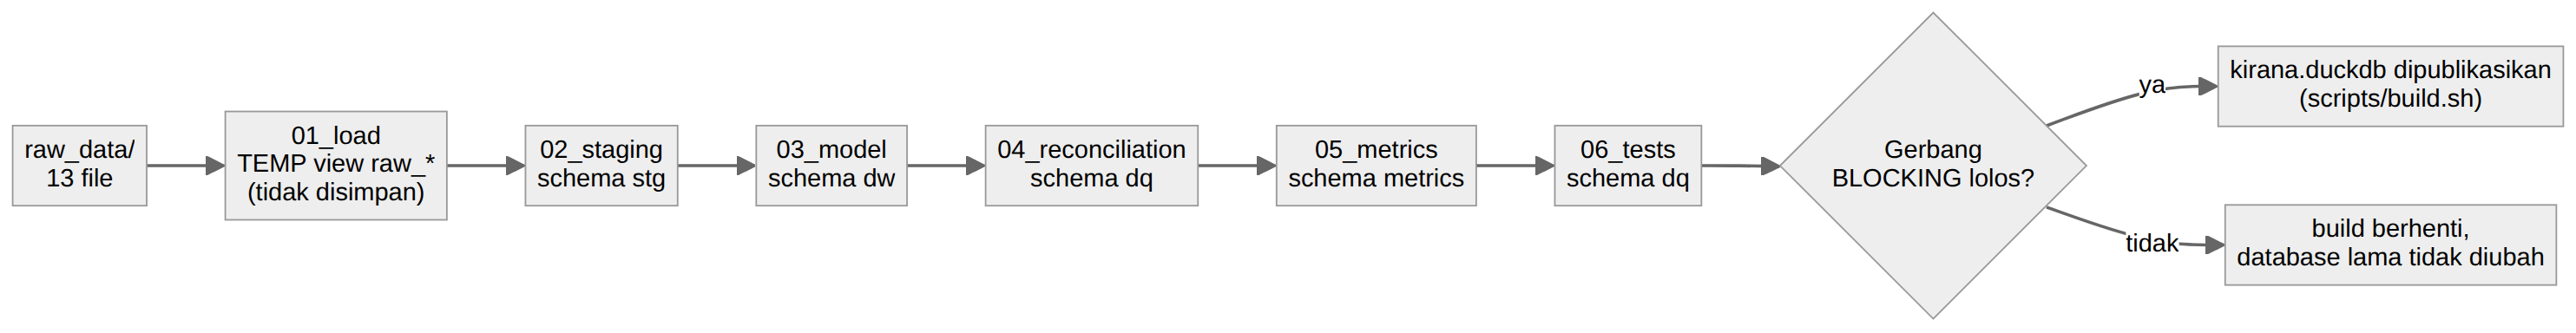
\includegraphics[keepaspectratio,alt={Diagram alur data}]{img/mermaid1.png}}
\caption{Diagram alur data}
\end{figure}

{\def\LTcaptype{none} % do not increment counter
\begin{longtable}[]{@{}
  >{\raggedright\arraybackslash}p{(\linewidth - 6\tabcolsep) * \real{0.1100}}
  >{\raggedright\arraybackslash}p{(\linewidth - 6\tabcolsep) * \real{0.1700}}
  >{\raggedright\arraybackslash}p{(\linewidth - 6\tabcolsep) * \real{0.3600}}
  >{\raggedright\arraybackslash}p{(\linewidth - 6\tabcolsep) * \real{0.3600}}@{}}
\toprule\noalign{}
\begin{minipage}[b]{\linewidth}\raggedright
Lapisan
\end{minipage} & \begin{minipage}[b]{\linewidth}\raggedright
File
\end{minipage} & \begin{minipage}[b]{\linewidth}\raggedright
Isi
\end{minipage} & \begin{minipage}[b]{\linewidth}\raggedright
Catatan
\end{minipage} \\
\midrule\noalign{}
\endhead
\bottomrule\noalign{}
\endlastfoot
load & \href{https://github.com/titan2903/kirana-omnichannel-performance-intelligence/blob/master/sql/01_load.sql}{\texttt{01\_\allowbreak{}load.sql}} & View \texttt{raw\_\allowbreak{}*} atas file CSV/XLSX, semua kolom VARCHAR & \textbf{TEMP}: tidak ikut tersimpan. Raw memuat PII dan path \texttt{raw\_\allowbreak{}data/} yang tidak ada di container Metabase \\
staging & \href{https://github.com/titan2903/kirana-omnichannel-performance-intelligence/blob/master/sql/02_staging.sql}{\texttt{02\_\allowbreak{}staging.sql}} & Normalisasi, tipe, dedup, pasangan void, karantina; \texttt{disposition} per baris & Tiap perlakuan diberi komentar \texttt{-\/-\ DQ-xx} \\
model & \href{https://github.com/titan2903/kirana-omnichannel-performance-intelligence/blob/master/sql/03_model.sql}{\texttt{03\_\allowbreak{}model.sql}} & Dimensi dan fakta (star schema) & Tanpa PII \\
rekonsiliasi & \href{https://github.com/titan2903/kirana-omnichannel-performance-intelligence/blob/master/sql/04_reconciliation.sql}{\texttt{04\_\allowbreak{}reconciliation.sql}} & \texttt{dq.reconciliation}, \texttt{dq.net\_\allowbreak{}sales\_\allowbreak{}bridge} & Sisi mentah dihitung dari raw, bukan dari stg \\
semantic layer & \href{https://github.com/titan2903/kirana-omnichannel-performance-intelligence/blob/master/sql/05_metrics.sql}{\texttt{05\_\allowbreak{}metrics.sql}} & \texttt{metrics.v\_\allowbreak{}*}, \texttt{metrics.ref\_\allowbreak{}status\_\allowbreak{}threshold}, \texttt{metrics.kpi\_\allowbreak{}dictionary} & Satu-satunya tempat rumus KPI; lihat A7 \\
uji & \href{https://github.com/titan2903/kirana-omnichannel-performance-intelligence/blob/master/sql/06_tests.sql}{\texttt{06\_\allowbreak{}tests.sql}} & \texttt{dq.test\_\allowbreak{}results}, \texttt{dq.test\_\allowbreak{}results\_\allowbreak{}demo} & Gerbang di \href{https://github.com/titan2903/kirana-omnichannel-performance-intelligence/blob/master/sql/00_main.sql}{\texttt{00\_\allowbreak{}main.sql}}; 43 uji, termasuk 15 uji semantic layer, region, dan akses (T40--T54) \\
\end{longtable}
}

\texttt{kirana.duckdb} memuat schema \texttt{stg}, \texttt{dw}, \texttt{dq}, \texttt{metrics}, dan enam schema akses \texttt{acc\_\allowbreak{}\textless{}region\textgreater{}} (Task 6). Tidak ada kolom PII di database ini.

\subsection{2. Star schema}\label{star-schema}

\begin{figure}
\centering
\pandocbounded{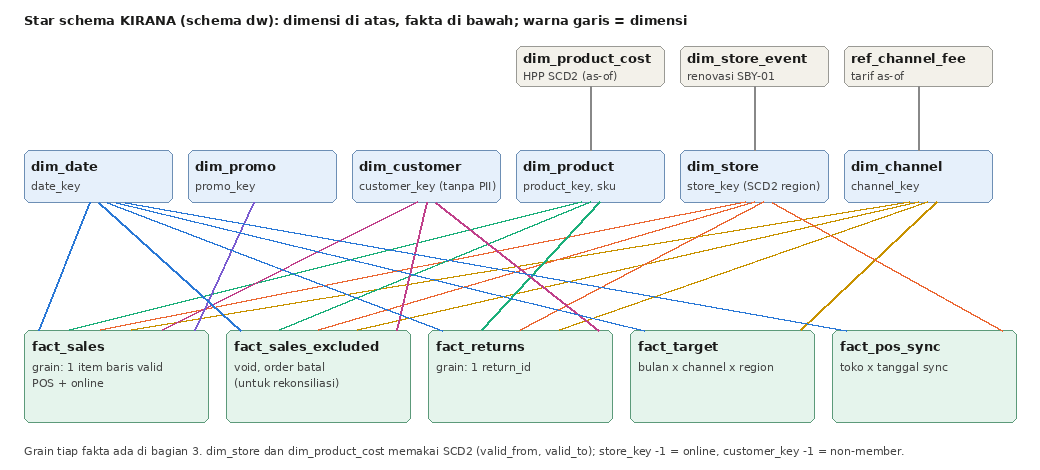
\includegraphics[keepaspectratio,alt={Star schema}]{img/star_schema.png}}
\caption{Star schema}
\end{figure}

{\def\LTcaptype{none} % do not increment counter
\begin{longtable}[]{@{}
  >{\raggedright\arraybackslash}p{(\linewidth - 4\tabcolsep) * \real{0.2871}}
  >{\raggedleft\arraybackslash}p{(\linewidth - 4\tabcolsep) * \real{0.1188}}
  >{\raggedright\arraybackslash}p{(\linewidth - 4\tabcolsep) * \real{0.5941}}@{}}
\toprule\noalign{}
\begin{minipage}[b]{\linewidth}\raggedright
Tabel
\end{minipage} & \begin{minipage}[b]{\linewidth}\raggedleft
Baris
\end{minipage} & \begin{minipage}[b]{\linewidth}\raggedright
Kunci
\end{minipage} \\
\midrule\noalign{}
\endhead
\bottomrule\noalign{}
\endlastfoot
\texttt{dw.fact\_\allowbreak{}sales} & 455.050 & \texttt{sales\_\allowbreak{}key}; grain \texttt{(source\_\allowbreak{}system,\ txn\_\allowbreak{}id,\ line\_\allowbreak{}no,\ product\_\allowbreak{}key)} \\
\texttt{dw.fact\_\allowbreak{}sales\_\allowbreak{}excluded} & 16.867 & \texttt{excluded\_\allowbreak{}key} \\
\texttt{dw.fact\_\allowbreak{}returns} & 18.089 & \texttt{return\_\allowbreak{}key} / \texttt{return\_\allowbreak{}id} \\
\texttt{dw.fact\_\allowbreak{}target} & 162 & \texttt{target\_\allowbreak{}key}; \texttt{(month\_\allowbreak{}start,\ channel\_\allowbreak{}key,\ region)} \\
\texttt{dw.fact\_\allowbreak{}pos\_\allowbreak{}sync} & 16.036 & \texttt{sync\_\allowbreak{}key}; \texttt{(store\_\allowbreak{}code,\ business\_\allowbreak{}date)} \\
\texttt{dw.dim\_\allowbreak{}date} & 1.096 & \texttt{date\_\allowbreak{}key} (yyyymmdd), 2024-01-01 s.d. 2026-12-31 \\
\texttt{dw.dim\_\allowbreak{}product} & 600 & \texttt{product\_\allowbreak{}key}, \texttt{sku} \\
\texttt{dw.dim\_\allowbreak{}product\_\allowbreak{}cost} & 850 & SCD2 HPP \\
\texttt{dw.dim\_\allowbreak{}store} & 20 & SCD2 region; \texttt{store\_\allowbreak{}key} -1 = online \\
\texttt{dw.dim\_\allowbreak{}channel} & 4 & Store, Website, Mobile App, Marketplace \\
\texttt{dw.dim\_\allowbreak{}customer} & 42.321 & tanpa PII; \texttt{customer\_\allowbreak{}key} -1 = non-member \\
\texttt{dw.dim\_\allowbreak{}promo} & 75 & 73 promo + \texttt{B2B-CORP} + \texttt{NONE} (-1) \\
\texttt{dw.ref\_\allowbreak{}channel\_\allowbreak{}fee} & 5 & tarif as-of per channel \\
\texttt{dw.dim\_\allowbreak{}store\_\allowbreak{}event} & 1 & renovasi SBY-01 \\
\end{longtable}
}

\subsection{3. Pernyataan grain}\label{pernyataan-grain}

{\def\LTcaptype{none} % do not increment counter
\begin{longtable}[]{@{}
  >{\raggedright\arraybackslash}p{(\linewidth - 2\tabcolsep) * \real{0.3000}}
  >{\raggedright\arraybackslash}p{(\linewidth - 2\tabcolsep) * \real{0.7000}}@{}}
\toprule\noalign{}
\begin{minipage}[b]{\linewidth}\raggedright
Fakta
\end{minipage} & \begin{minipage}[b]{\linewidth}\raggedright
Grain
\end{minipage} \\
\midrule\noalign{}
\endhead
\bottomrule\noalign{}
\endlastfoot
\texttt{fact\_\allowbreak{}sales} & \textbf{Satu baris = satu item baris transaksi valid}: POS \texttt{trx\_\allowbreak{}id\ +\ line\_\allowbreak{}no\ +\ sku}, online \texttt{order\_\allowbreak{}no\ +\ line\_\allowbreak{}no\ +\ sku}. Valid berarti sudah dedup, bukan void maupun baris asli yang di-void, bukan order \texttt{CANCELLED}, dan toko ada di master. POS dan online berada dalam satu tabel dengan kolom \texttt{source\_\allowbreak{}system} \\
\texttt{fact\_\allowbreak{}sales\_\allowbreak{}excluded} & Satu baris = satu item baris yang \textbf{bukan penjualan} (void, baris asli yang di-void, order batal). Dipakai untuk cancellation rate dan void rate \\
\texttt{fact\_\allowbreak{}returns} & Satu baris = satu \texttt{return\_\allowbreak{}id} (retur per item) yang terhubung ke penjualan valid \\
\texttt{fact\_\allowbreak{}target} & Satu baris = satu bulan x channel x (region untuk Store, \texttt{Nasional} untuk online) \\
\texttt{fact\_\allowbreak{}pos\_\allowbreak{}sync} & Satu baris = satu toko x tanggal bisnis di sync log \\
\end{longtable}
}

Kolom ukuran di \texttt{fact\_\allowbreak{}sales}: \texttt{qty}, \texttt{unit\_\allowbreak{}price}, \texttt{gross\_\allowbreak{}sales}, \texttt{discount}, \texttt{net\_\allowbreak{}sales}, \texttt{unit\_\allowbreak{}cost}, \texttt{cogs},
\texttt{gross\_\allowbreak{}margin}, \texttt{channel\_\allowbreak{}fee\_\allowbreak{}pct}, \texttt{channel\_\allowbreak{}fee}. Flag: \texttt{is\_\allowbreak{}member}, \texttt{is\_\allowbreak{}b2b\_\allowbreak{}bulk}, \texttt{key\_\allowbreak{}collision},
\texttt{province\_\allowbreak{}source}. Region: \texttt{region\_\allowbreak{}target\_\allowbreak{}basis} (dasar achievement), \texttt{region\_\allowbreak{}asof}, dan \texttt{region\_\allowbreak{}current}.

\subsection{4. Keputusan pembersihan yang diterapkan di staging}\label{keputusan-pembersihan-yang-diterapkan-di-staging}

{\def\LTcaptype{none} % do not increment counter
\begin{longtable}[]{@{}
  >{\raggedright\arraybackslash}p{(\linewidth - 4\tabcolsep) * \real{0.1000}}
  >{\raggedright\arraybackslash}p{(\linewidth - 4\tabcolsep) * \real{0.4500}}
  >{\raggedright\arraybackslash}p{(\linewidth - 4\tabcolsep) * \real{0.4500}}@{}}
\toprule\noalign{}
\begin{minipage}[b]{\linewidth}\raggedright
ID
\end{minipage} & \begin{minipage}[b]{\linewidth}\raggedright
Perlakuan di \href{https://github.com/titan2903/kirana-omnichannel-performance-intelligence/blob/master/sql/02_staging.sql}{\texttt{02\_\allowbreak{}staging.sql}}
\end{minipage} & \begin{minipage}[b]{\linewidth}\raggedright
Hasil
\end{minipage} \\
\midrule\noalign{}
\endhead
\bottomrule\noalign{}
\endlastfoot
DQ-01, 03 & \texttt{upper(trim())} pada \texttt{store\_\allowbreak{}code} dan \texttt{sku} & Semua SKU cocok ke master; toko terpetakan \\
DQ-02 & \texttt{TRN-99} → \texttt{REJECT\_\allowbreak{}STORE\_\allowbreak{}NOT\_\allowbreak{}IN\_\allowbreak{}MASTER} & 320 baris (324 dengan salinan) dikarantina \\
DQ-04, 10 & Dedup persis (\texttt{GROUP\ BY\ ALL}, \texttt{n\_\allowbreak{}copies}) & 1.577 POS dan 232 online salinan ekstra \\
DQ-05 & Tabrakan nomor struk dipertahankan, ditandai \texttt{key\_\allowbreak{}collision} & 20 grup; seluruhnya melibatkan pasangan void sehingga tidak ada di \texttt{fact\_\allowbreak{}sales} \\
DQ-06 & Void dipasangkan 1:1 dengan baris asli (\texttt{trx\_\allowbreak{}id}, \texttt{sku}, \texttt{qty} berlawanan) & 2.067 void dan 2.067 baris asli dikeluarkan \\
DQ-07 & B2B bulk dipertahankan, \texttt{is\_\allowbreak{}b2b\_\allowbreak{}bulk} & 14 baris, \texttt{B2B-CORP} masuk \texttt{dim\_\allowbreak{}promo} \\
DQ-08 & Pemetaan eksplisit 12 label channel & Label tak dikenal → \texttt{REJECT\_\allowbreak{}UNMAPPED\_\allowbreak{}CHANNEL} (diuji) \\
DQ-09 & Parser harga hanya dua pola (\texttt{100900}, \texttt{Rp100.900}) & Pola lain → \texttt{REJECT\_\allowbreak{}UNPARSEABLE} (diuji) \\
DQ-11 & Order \texttt{CANCELLED} → \texttt{EXCLUDE\_\allowbreak{}CANCELLED} & 12.733 baris, disimpan di \texttt{fact\_\allowbreak{}sales\_\allowbreak{}excluded} \\
DQ-12 & Provinsi kosong \textbf{disimpulkan dari \texttt{ship\_\allowbreak{}city}} bila kota hanya berpasangan dengan satu provinsi & Seluruh 1.984 baris terselesaikan (\texttt{province\_\allowbreak{}source\ =\ INFERRED\_\allowbreak{}FROM\_\allowbreak{}CITY}) \\
DQ-13, 14 & Satu baris per SKU (buang varian \texttt{(old)}), kategori dibakukan & 600 SKU; 6 dikarantina \\
DQ-16 & Target di-unpivot, label region dibakukan & 162 sel \\
DQ-18, 19 & \texttt{age\_\allowbreak{}band} dari \texttt{birth\_\allowbreak{}date}; flag \texttt{possible\_\allowbreak{}duplicate\_\allowbreak{}member} dari email ganda; PII dibuang & 418 \texttt{Tidak\ diketahui}; 982 member ditandai \\
DQ-21, 22 & Retur yatim dikarantina; label alasan digabung & 1 retur ditolak \\
\end{longtable}
}

\textbf{Pemetaan region online.} Region ditentukan dari \textbf{provinsi tujuan} sesuai panduan paket data. Banten → Jabodetabek
(satu-satunya kota di data adalah Tangerang, sama dengan toko TGR-01); Sulawesi Selatan dan Kalimantan Timur → \texttt{Lainnya}.
Keterbatasan: kota Bekasi, Bogor, dan Depok berada di provinsi Jawa Barat sehingga masuk region \texttt{Jawa\ Barat}, padahal
toko di kota yang sama berada di \texttt{Jabodetabek}. Target online ditetapkan per channel nasional, sehingga ini hanya
memengaruhi analisis regional online, bukan perhitungan achievement.

\subsection{5. Keputusan SCD dan dampaknya}\label{keputusan-scd-dan-dampaknya}

Dampak dihitung oleh \href{https://github.com/titan2903/kirana-omnichannel-performance-intelligence/blob/master/sql/analysis/scd_impact.sql}{\texttt{sql/analysis/scd\_\allowbreak{}impact.sql}}.

\subsubsection{\texorpdfstring{(a) HPP: \texttt{product\_\allowbreak{}cost\_\allowbreak{}history} (SCD tipe 2)}{(a) HPP: product\_\allowbreak{}cost\_\allowbreak{}history (SCD tipe 2)}}\label{a-hpp-product_cost_history-scd-tipe-2}

\textbf{Keputusan:} COGS = \texttt{qty\ x\ HPP\ yang\ berlaku\ pada\ tanggal\ transaksi} (\texttt{dim\_\allowbreak{}product\_\allowbreak{}cost}, join \texttt{BETWEEN\ valid\_\allowbreak{}from\ AND\ valid\_\allowbreak{}to}).
\texttt{products.current\_\allowbreak{}unit\_\allowbreak{}cost} (HPP per 30 Jun 2026) \textbf{tidak} dipakai untuk histori.

{\def\LTcaptype{none} % do not increment counter
\begin{longtable}[]{@{}
  >{\raggedright\arraybackslash}p{(\linewidth - 8\tabcolsep) * \real{0.0962}}
  >{\raggedleft\arraybackslash}p{(\linewidth - 8\tabcolsep) * \real{0.2019}}
  >{\raggedleft\arraybackslash}p{(\linewidth - 8\tabcolsep) * \real{0.2885}}
  >{\raggedleft\arraybackslash}p{(\linewidth - 8\tabcolsep) * \real{0.2981}}
  >{\raggedleft\arraybackslash}p{(\linewidth - 8\tabcolsep) * \real{0.1154}}@{}}
\toprule\noalign{}
\begin{minipage}[b]{\linewidth}\raggedright
Periode
\end{minipage} & \begin{minipage}[b]{\linewidth}\raggedleft
Net Sales
\end{minipage} & \begin{minipage}[b]{\linewidth}\raggedleft
Gross margin as-of (dipakai)
\end{minipage} & \begin{minipage}[b]{\linewidth}\raggedleft
Gross margin bila HPP terkini
\end{minipage} & \begin{minipage}[b]{\linewidth}\raggedleft
Selisih
\end{minipage} \\
\midrule\noalign{}
\endhead
\bottomrule\noalign{}
\endlastfoot
FY2024 & Rp 37.619.579.300 & \textbf{46,11\%} & 43,03\% & −3,07 pt \\
FY2025 & Rp 43.957.237.300 & \textbf{44,32\%} & 42,49\% & −1,83 pt \\
H1 2026 & Rp 25.210.478.100 & \textbf{43,05\%} & 43,05\% & 0,00 pt \\
\end{longtable}
}

\begin{itemize}
\tightlist
\item
  Sebanyak 126.374 baris (27,8\%) memiliki HPP yang berbeda antara as-of dan terkini. 250 SKU mengalami kenaikan HPP (60 SKU pada 1 Jul 2025, rata-rata +18\%; 190 SKU pada 1 Jan 2026, rata-rata +4\%).
\item
  \textbf{Dampak bagi cerita bisnis:} dengan HPP as-of, gross margin turun 3,06 pt dari 2024 ke H1 2026 (46,11\% → 43,05\%), yaitu gejala ``margin kotor menurun'' yang diminta manajemen. Dengan HPP terkini, penurunan itu hampir hilang (43,03\% → 42,49\% → 43,05\%) karena seluruh histori dinilai memakai HPP tertinggi. Memakai \texttt{current\_\allowbreak{}unit\_\allowbreak{}cost} akan menyembunyikan masalah yang justru harus dijelaskan.
\end{itemize}

\subsubsection{\texorpdfstring{(b) Region toko: \texttt{store\_\allowbreak{}region\_\allowbreak{}history} (SCD tipe 2)}{(b) Region toko: store\_\allowbreak{}region\_\allowbreak{}history (SCD tipe 2)}}\label{b-region-toko-store_region_history-scd-tipe-2}

\begin{quote}
\textbf{Koreksi (Task 5).} Keputusan awal di Task 2 memakai region \emph{saat transaksi} untuk membandingkan penjualan dengan target. Analisis Task 5
menunjukkan itu salah: target FP\&A \textbf{tidak disesuaikan} ketika BGR-01 pindah (1 Jul 2025). Target Jawa Barat tetap 341 juta (Jun 2025) dan 347
juta (Jul 2025), baru turun menjadi 277 juta pada Jan 2026 (Des 2025: 439 juta). Target Jabodetabek tidak melonjak pada Juli 2025 (792 → 821 juta).
Jadi target FY2025 disusun dengan peta region lama sepanjang tahun, dan target 2026 dengan peta baru.
\end{quote}

\textbf{Keputusan (direvisi):} \texttt{dim\_\allowbreak{}store} SCD2 tetap dipakai, tetapi tiga kolom region disimpan di fakta:

{\def\LTcaptype{none} % do not increment counter
\begin{longtable}[]{@{}
  >{\raggedright\arraybackslash}p{(\linewidth - 4\tabcolsep) * \real{0.1800}}
  >{\raggedright\arraybackslash}p{(\linewidth - 4\tabcolsep) * \real{0.4100}}
  >{\raggedright\arraybackslash}p{(\linewidth - 4\tabcolsep) * \real{0.4100}}@{}}
\toprule\noalign{}
\begin{minipage}[b]{\linewidth}\raggedright
Kolom
\end{minipage} & \begin{minipage}[b]{\linewidth}\raggedright
Arti
\end{minipage} & \begin{minipage}[b]{\linewidth}\raggedright
Dipakai untuk
\end{minipage} \\
\midrule\noalign{}
\endhead
\bottomrule\noalign{}
\endlastfoot
\texttt{region\_\allowbreak{}target\_\allowbreak{}basis} & Region toko pada \textbf{awal tahun} transaksi (1 Jan, atau \texttt{open\_\allowbreak{}date} bila toko buka belakangan) = peta yang berlaku saat target tahun itu disusun & Achievement vs target, alokasi target toko, dan filter Region dashboard \\
\texttt{region\_\allowbreak{}asof} & Region saat transaksi terjadi & Deskriptif (lokasi operasional pada saat itu) \\
\texttt{region\_\allowbreak{}current} & Region per 30 Jun 2026 & Pembanding \\
\end{longtable}
}

Bukti (\href{https://github.com/titan2903/kirana-omnichannel-performance-intelligence/blob/master/sql/analysis/scd_impact.sql}{\texttt{sql/analysis/scd\_\allowbreak{}impact.sql}}; uji \texttt{T53} menjaganya): achievement per semester, Store terhadap target region.

{\def\LTcaptype{none} % do not increment counter
\begin{longtable}[]{@{}
  >{\raggedright\arraybackslash}p{(\linewidth - 8\tabcolsep) * \real{0.1262}}
  >{\raggedright\arraybackslash}p{(\linewidth - 8\tabcolsep) * \real{0.0874}}
  >{\raggedleft\arraybackslash}p{(\linewidth - 8\tabcolsep) * \real{0.2427}}
  >{\raggedleft\arraybackslash}p{(\linewidth - 8\tabcolsep) * \real{0.3495}}
  >{\raggedleft\arraybackslash}p{(\linewidth - 8\tabcolsep) * \real{0.1942}}@{}}
\toprule\noalign{}
\begin{minipage}[b]{\linewidth}\raggedright
Region
\end{minipage} & \begin{minipage}[b]{\linewidth}\raggedright
Periode
\end{minipage} & \begin{minipage}[b]{\linewidth}\raggedleft
A: region saat transaksi
\end{minipage} & \begin{minipage}[b]{\linewidth}\raggedleft
\textbf{B: peta awal tahun target (dipakai)}
\end{minipage} & \begin{minipage}[b]{\linewidth}\raggedleft
C: region saat ini
\end{minipage} \\
\midrule\noalign{}
\endhead
\bottomrule\noalign{}
\endlastfoot
Jawa Barat & H1 2025 & 98,1\% & \textbf{98,1\%} & 70,9\% \\
Jawa Barat & H2 2025 & 73,4\% & \textbf{103,4\%} & 73,4\% \\
Jawa Barat & H1 2026 & 95,8\% & \textbf{95,8\%} & 95,8\% \\
Jabodetabek & H1 2025 & 94,9\% & \textbf{94,9\%} & 107,0\% \\
Jabodetabek & H2 2025 & 109,7\% & \textbf{96,3\%} & 109,7\% \\
Jabodetabek & H1 2026 & 96,7\% & \textbf{96,7\%} & 96,7\% \\
\end{longtable}
}

\begin{itemize}
\tightlist
\item
  Pemetaan A menciptakan \textbf{lonjakan palsu} tepat di titik pindah (Jawa Barat 98,1\% → 73,4\%, Jabodetabek 94,9\% → 109,7\%). Pemetaan B stabil di kedua sisi.
\item
  FY2025: Jawa Barat \textbf{100,8\%} (A: 85,6\%; C: 72,2\%) dan Jabodetabek \textbf{95,6\%} (A: 102,4\%; C: 108,4\%). Selisih berasal dari Rp 673.004.400 penjualan BGR-01 pada Juli--Desember 2025.
\item
  \textbf{Dampak bagi keputusan:} dengan pemetaan A, Jawa Barat tampak sebagai region merah pada FY2025; dengan pemetaan yang benar, ia tidak bermasalah, dan Jabodetabek yang terlihat hijau sebenarnya Kuning.
\item
  Toko tanpa riwayat memakai \texttt{stores.region} sejak \texttt{open\_\allowbreak{}date}. Online memakai region dari provinsi tujuan (target online nasional per channel).
\end{itemize}

\subsubsection{(c) Biaya channel}\label{c-biaya-channel}

Tarif dipasang per baris menurut tanggal transaksi (\texttt{ref\_\allowbreak{}channel\_\allowbreak{}fee}); Marketplace 9,0\% sampai 31 Mar 2025 dan 11,5\% sejak 1 Apr 2025.

\subsection{6. Keterbatasan yang diketahui}\label{keterbatasan-yang-diketahui}

\begin{itemize}
\tightlist
\item
  \textbf{Pasangan void bisa ambigu.} Void dipasangkan dengan baris asli berdasarkan \texttt{(trx\_\allowbreak{}id,\ sku,\ qty\ berlawanan)} dan urutan baris. Ada 379 kelompok \texttt{(trx\_\allowbreak{}id,\ sku,\ qty)} dengan lebih dari satu baris asli atau void; hanya 10 kelompok yang barisnya asli lebih banyak dari void, dan hanya 3 di antaranya bernilai berbeda. Eksposur terburuk \textbf{Rp 38.500} (jauh di bawah 0,0001\% Net Sales). Jumlah baris dijamin benar oleh kontrol sync log (T13).
\item
  \textbf{Void tidak selalu meniadakan nilai asli.} Tiga void dicatat sumber dengan harga penuh tanpa diskon, sehingga void dan baris aslinya tidak persis saling meniadakan (selisih bersih −Rp 22.500). Keduanya tetap dikeluarkan dari Net Sales.
\item
  \textbf{Region online berdasarkan provinsi}, bukan kota (lihat §4). Banten hanya berisi Tangerang di data ini; bila muncul kota Banten lain (mis. Serang), pemetaan ke Jabodetabek perlu ditinjau.
\item
  \textbf{Ekstensi \texttt{excel} diunduh sekali} pada mesin baru (\texttt{INSTALL\ excel}); setelah terpasang, build tidak membutuhkan jaringan (diuji dengan repository yang tidak terjangkau).
\end{itemize}

\subsection{7. Sumber diagram}\label{sumber-diagram}

Diagram star schema dan lineage dibuat sebagai draw.io (\href{https://github.com/titan2903/kirana-omnichannel-performance-intelligence/blob/master/reports/img/star_schema.drawio}{\texttt{reports/img/star\_\allowbreak{}schema.drawio}}, \href{https://github.com/titan2903/kirana-omnichannel-performance-intelligence/blob/master/reports/img/lineage.drawio}{\texttt{lineage.drawio}}) dan diekspor ke PNG oleh \href{https://github.com/titan2903/kirana-omnichannel-performance-intelligence/blob/master/reports/img/build_star.py}{\texttt{reports/img/build\_\allowbreak{}star.py}} dan \href{https://github.com/titan2903/kirana-omnichannel-performance-intelligence/blob/master/reports/img/build_lineage.py}{\texttt{build\_\allowbreak{}lineage.py}}.

% ======== A5_quality_reconciliation ========
\section{A5. Uji Kualitas Data dan Rekonsiliasi}\label{a5.-uji-kualitas-data-dan-rekonsiliasi}

Dihasilkan oleh \href{https://github.com/titan2903/kirana-omnichannel-performance-intelligence/blob/master/sql/04_reconciliation.sql}{\texttt{sql/04\_\allowbreak{}reconciliation.sql}} dan \href{https://github.com/titan2903/kirana-omnichannel-performance-intelligence/blob/master/sql/06_tests.sql}{\texttt{sql/06\_\allowbreak{}tests.sql}}; tabel hasil ada di \texttt{kirana.duckdb}
(\texttt{dq.reconciliation}, \texttt{dq.net\_\allowbreak{}sales\_\allowbreak{}bridge}, \texttt{dq.test\_\allowbreak{}results}, \texttt{dq.test\_\allowbreak{}results\_\allowbreak{}demo}).

\begin{Verbatim}[commandchars=\\\{\},breaklines,fontsize=\scriptsize]
bash \gh{scripts/build.sh}                                          # bangun ke file sementara; kirana.duckdb diganti HANYA bila semua uji BLOCKING lolos
bash \gh{scripts/mutation_test.sh}                                  # 39 cacat disuntik ke salinan (data, staging, semantic layer, region, dan akses); semua harus terdeteksi
duckdb -readonly kirana.duckdb -markdown -c "SELECT * FROM dq.test_results ORDER BY test_id"
bash \gh{scripts/idempotency_check.sh}   # IDEMPOTENT: 62 objek identik di dua run
\end{Verbatim}

\subsection{1. Hasil uji produksi}\label{hasil-uji-produksi}

\textbf{43 uji: 29 BLOCKING (semua lolos), 14 WARNING (11 lolos, 3 temuan yang sudah diketahui).}

\emph{BLOCKING = bila diabaikan, angka akan salah, sehingga build berhenti. WARNING = angka tetap valid, tetapi ada kondisi sumber yang harus dicatat; baris ditandai atau dikarantina, bukan dibuang.}

{\def\LTcaptype{none} % do not increment counter
\begin{longtable}[]{@{}
  >{\raggedright\arraybackslash}p{(\linewidth - 10\tabcolsep) * \real{0.0400}}
  >{\raggedright\arraybackslash}p{(\linewidth - 10\tabcolsep) * \real{0.3500}}
  >{\raggedright\arraybackslash}p{(\linewidth - 10\tabcolsep) * \real{0.0700}}
  >{\raggedleft\arraybackslash}p{(\linewidth - 10\tabcolsep) * \real{0.0700}}
  >{\raggedright\arraybackslash}p{(\linewidth - 10\tabcolsep) * \real{0.1200}}
  >{\raggedright\arraybackslash}p{(\linewidth - 10\tabcolsep) * \real{0.3500}}@{}}
\toprule\noalign{}
\begin{minipage}[b]{\linewidth}\raggedright
ID
\end{minipage} & \begin{minipage}[b]{\linewidth}\raggedright
Uji
\end{minipage} & \begin{minipage}[b]{\linewidth}\raggedright
Severity
\end{minipage} & \begin{minipage}[b]{\linewidth}\raggedleft
Gagal
\end{minipage} & \begin{minipage}[b]{\linewidth}\raggedright
Status
\end{minipage} & \begin{minipage}[b]{\linewidth}\raggedright
Alasan
\end{minipage} \\
\midrule\noalign{}
\endhead
\bottomrule\noalign{}
\endlastfoot
T01 & Grain \texttt{fact\_\allowbreak{}sales} unik (source, txn\_\allowbreak{}id, line\_\allowbreak{}no, produk) & BLOCKING & 0 & PASS & Duplikat menggandakan revenue \\
T02 & Tidak ada FK yatim (tanggal, produk, toko, channel, pelanggan, promo) & BLOCKING & 0 & PASS & Baris yatim hilang dari agregat \\
T03 & Channel, toko, region hanya bernilai resmi & BLOCKING & 0 & PASS & Memecah agregat (DQ-01, 08) \\
T04 & Tiap baris punya tepat satu HPP as-of dan sama dengan nilai di fakta & BLOCKING & 0 & PASS & COGS dan GM salah (SCD HPP) \\
T05 & Tiap baris punya tarif biaya channel as-of & BLOCKING & 0 & PASS & Contribution margin menyimpang \\
T10 & Rekonsiliasi raw → fakta: selisih baris dan Rp = 0 & BLOCKING & 0 & PASS & Data hilang tanpa jejak \\
T11 & Jembatan Net Sales menutup & BLOCKING & 0 & PASS & Net Sales harus dapat ditelusuri \\
T12 & Tidak ada kolom PII langsung di stg/dw/dq/metrics/acc\_\allowbreak{}* & BLOCKING & 0 & PASS & PII tidak boleh ke dashboard \\
T13 & Kontrol sync log: \texttt{SUM(rows\_\allowbreak{}uploaded)} = baris POS valid tanpa B2B & BLOCKING & 0 & PASS & Kontrol independen dari IT: membuktikan dedup dan void benar \\
T14 & \texttt{dim\_\allowbreak{}store} SCD2: satu region per toko per tanggal, tanpa tumpang tindih & BLOCKING & 0 & PASS & Region salah memindahkan penjualan antar target (DQ-15) \\
T15 & Kunci alami dimensi unik & BLOCKING & 0 & PASS & Kunci ganda menggandakan fakta (DQ-13) \\
T16 & \texttt{fact\_\allowbreak{}target} lengkap, unik, total sama dengan Excel & BLOCKING & 0 & PASS & Achievement kosong (DQ-16) \\
T17 & Retur terhubung ke penjualan asal dan konsisten & BLOCKING & 0 & PASS & Retur tanpa asal tak bisa dikelompokkan \\
T18 & Tidak ada baris ditolak karena format/label tak dikenal & BLOCKING & 0 & PASS & Label baru harus ditangani eksplisit \\
T19 & \texttt{return\_\allowbreak{}id} unik di \texttt{fact\_\allowbreak{}returns} & BLOCKING & 0 & PASS & Retur ganda menggandakan refund; rekonsiliasi tidak mendeteksinya karena raw dan fakta sama-sama memuat duplikat \\
T20 & Net sales ≥ 0 dan diskon ≤ gross & WARNING & 0 & PASS & Anomali nilai \\
T21 & Retur yatim & WARNING & \textbf{1} & FAIL (diketahui) & DQ-21: dikarantina, tidak masuk \texttt{fact\_\allowbreak{}returns} \\
T22 & Hari sync POS FAILED & WARNING & \textbf{7} & FAIL (diketahui) & DQ-23: BDG-02, 3--9 Nov 2025; tidak diimputasi, ditandai data tidak lengkap \\
T23 & Tabrakan nomor struk di \texttt{fact\_\allowbreak{}sales} & WARNING & 0 & PASS & DQ-05: 20 grup, semuanya pasangan void sehingga tidak ada di fakta \\
T24 & Void tanpa baris asli di toko master & WARNING & 0 & PASS & DQ-06c: satu-satunya kasus ada di \texttt{TRN-99} \\
T25 & Provinsi online tak terselesaikan & WARNING & 0 & PASS & DQ-12: seluruhnya terselesaikan dari kota \\
T26 & Promo dipakai di luar masa berlaku, channel, member-only, atau kategori & WARNING & 0 & PASS & Menyesatkan analisis promo \\
T27 & Penjualan valid sebelum \texttt{launch\_\allowbreak{}date} & WARNING & 0 & PASS & DQ-17 \\
T28 & Target lengkap 18 bulan x 9 baris & WARNING & 0 & PASS & Achievement NULL \\
T29 & Transaksi B2B bulk di fakta & WARNING & \textbf{14} & FAIL (diketahui) & DQ-07: dipertahankan, ditandai \texttt{is\_\allowbreak{}b2b\_\allowbreak{}bulk} \\
T30 & Retur atas penjualan yang sudah dikeluarkan (void/batal) & WARNING & 0 & PASS & Dikarantina bila terjadi; tidak boleh mengurangi Net Sales \\
T31 & Refund = qty retur x nilai bersih per unit (toleransi Rp 100) & WARNING & 0 & PASS & Refund menyimpang membuat Return Rate (Rp) bias \\
T32 & \texttt{promo\_\allowbreak{}type} dikenali & WARNING & 0 & PASS & Jenis promo baru jatuh ke \texttt{Lainnya} dan harus diperiksa \\
T40 & Kamus metrik memuat ≥ 8 KPI dan semua view yang dirujuk ada & BLOCKING & 0 & PASS & KPI tanpa view membuat angka dashboard tak dapat ditelusuri \\
T41 & \texttt{v\_\allowbreak{}sales\_\allowbreak{}monthly} = \texttt{fact\_\allowbreak{}sales} (Net Sales, gross margin, COGS, qty, diskon, fee) & BLOCKING & 0 & PASS & Baris hilang/ganda saat agregasi ke grain view \\
T42 & \texttt{v\_\allowbreak{}txn\_\allowbreak{}monthly} = \texttt{fact\_\allowbreak{}sales} (struk distinct, Net Sales) & BLOCKING & 0 & PASS & \texttt{transactions} hanya aditif bila satu struk jatuh di satu baris grain \\
T43 & \texttt{v\_\allowbreak{}target\_\allowbreak{}achievement}: aktual dan target menutup ke fakta & BLOCKING & 0 & PASS & Join target gagal membuat Achievement kosong/ganda \\
T44 & \texttt{v\_\allowbreak{}store\_\allowbreak{}target\_\allowbreak{}alloc}: pangsa = 1 dan target toko = target region & BLOCKING & 0 & PASS & Achievement toko harus konsisten dengan region \\
T45 & \texttt{v\_\allowbreak{}return\_\allowbreak{}rate\_\allowbreak{}monthly} dan \texttt{v\_\allowbreak{}return\_\allowbreak{}reason\_\allowbreak{}monthly} = \texttt{fact\_\allowbreak{}returns} & BLOCKING & 0 & PASS & Retur hilang membuat Return Rate terlalu rendah \\
T46 & Active Members tahunan = member unik langsung dari fakta & BLOCKING & 0 & PASS & Member unik tidak boleh dijumlahkan antar bulan \\
T47 & \texttt{v\_\allowbreak{}margin\_\allowbreak{}vs\_\allowbreak{}target} = fakta; target GM dan tarif ada untuk 2025-01..2026-06 & BLOCKING & 0 & PASS & Status margin yang salah menyesatkan keputusan promo \\
T48 & \texttt{v\_\allowbreak{}cancellation\_\allowbreak{}void\_\allowbreak{}monthly} = fakta (valid, batal, void) & BLOCKING & 0 & PASS & Rate harus berasal dari baris yang sama dengan rekonsiliasi \\
T49 & \texttt{v\_\allowbreak{}promo\_\allowbreak{}performance}: 73 promo dan total diskon = fakta & BLOCKING & 0 & PASS & Analisis efektivitas promo harus dapat dipercaya \\
T50 & Baseline Promo Lift memadai (tak ada TIDAK\_\allowbreak{}CUKUP) & WARNING & 0 & PASS & Promo tanpa baseline tidak punya lift \\
T51 & \texttt{v\_\allowbreak{}data\_\allowbreak{}completeness} konsisten dengan sync log & BLOCKING & 0 & PASS & Penanda data tidak lengkap harus sama dengan sumber \\
T52 & \texttt{v\_\allowbreak{}store\_\allowbreak{}performance\_\allowbreak{}monthly}: satu baris per bulan x toko; Net Sales dan target = \texttt{v\_\allowbreak{}store\_\allowbreak{}target\_\allowbreak{}alloc} & BLOCKING & 0 & PASS & Join kelengkapan yang menggandakan baris merusak achievement toko di dashboard \\
T53 & \texttt{region\_\allowbreak{}target\_\allowbreak{}basis} = region toko pada awal tahun transaksi (dihitung ulang dari \texttt{dim\_\allowbreak{}store}) & BLOCKING & 0 & PASS & Target FY2025 tidak disesuaikan saat BGR-01 pindah; region saat transaksi membuat achievement Jawa Barat dan Jabodetabek salah \\
T54 & Schema \texttt{acc\_\allowbreak{}\textless{}region\textgreater{}}: tiap view hanya memuat regionnya; gabungan semua region (+ Lainnya untuk online) = view induk & BLOCKING & 0 & PASS & Pembatasan akses per region yang bocor atau menghilangkan baris (Task 6) \\
\end{longtable}
}

Uji T13 menangkap bug nyata saat pengembangan: \texttt{is\_\allowbreak{}b2b\_\allowbreak{}bulk} bernilai NULL (bukan \texttt{false}) untuk baris tanpa promo,
sehingga 232 ribu baris POS tidak terhitung. Bug diperbaiki di staging dan uji kini lolos.

\subsection{2. Uji yang sengaja gagal}\label{uji-yang-sengaja-gagal}

Salinan \texttt{fact\_\allowbreak{}sales} disuntik tiga cacat (1 baris duplikat persis, 1 baris dengan \texttt{product\_\allowbreak{}key} 999999, 1 baris dengan
\texttt{net\_\allowbreak{}sales} −5.000). Macro uji yang sama dijalankan pada salinan itu; model produksi tidak berubah dan tetap PASS.

{\def\LTcaptype{none} % do not increment counter
\begin{longtable}[]{@{}
  >{\raggedright\arraybackslash}p{(\linewidth - 8\tabcolsep) * \real{0.0594}}
  >{\raggedright\arraybackslash}p{(\linewidth - 8\tabcolsep) * \real{0.2772}}
  >{\raggedleft\arraybackslash}p{(\linewidth - 8\tabcolsep) * \real{0.0891}}
  >{\raggedright\arraybackslash}p{(\linewidth - 8\tabcolsep) * \real{0.1089}}
  >{\raggedright\arraybackslash}p{(\linewidth - 8\tabcolsep) * \real{0.4653}}@{}}
\toprule\noalign{}
\begin{minipage}[b]{\linewidth}\raggedright
ID
\end{minipage} & \begin{minipage}[b]{\linewidth}\raggedright
Uji
\end{minipage} & \begin{minipage}[b]{\linewidth}\raggedleft
Gagal
\end{minipage} & \begin{minipage}[b]{\linewidth}\raggedright
Status
\end{minipage} & \begin{minipage}[b]{\linewidth}\raggedright
Cacat yang disuntik
\end{minipage} \\
\midrule\noalign{}
\endhead
\bottomrule\noalign{}
\endlastfoot
T01 & Grain unik & 1 & \textbf{FAIL} & 1 baris duplikat persis \\
T02 & FK yatim & 1 & \textbf{FAIL} & \texttt{product\_\allowbreak{}key} 999999 \\
T03 & Domain channel/toko/region & 0 & PASS & -- \\
T04 & HPP as-of & 1 & \textbf{FAIL} & akibat samping: tidak ada HPP untuk produk 999999 \\
T05 & Tarif biaya channel & 0 & PASS & -- \\
T20 & Net sales ≥ 0 & 1 & \textbf{FAIL} & \texttt{net\_\allowbreak{}sales} −5.000 \\
\end{longtable}
}

Hasil disimpan di \texttt{dq.test\_\allowbreak{}results\_\allowbreak{}demo}. Ini membuktikan uji benar-benar mendeteksi cacat, bukan sekadar selalu lolos.

\subsection{2b. Uji punya gigi: mutation test}\label{b.-uji-punya-gigi-mutation-test}

\href{https://github.com/titan2903/kirana-omnichannel-performance-intelligence/blob/master/scripts/mutation_test.sh}{\texttt{scripts/mutation\_\allowbreak{}test.sh}} menyuntik \textbf{satu cacat per percobaan} ke salinan \texttt{kirana.duckdb}, menjalankan ulang rekonsiliasi dan uji,
lalu memastikan uji yang tepat gagal. Hasil: \textbf{39 dari 39 cacat terdeteksi} (sekitar 1 menit; 24 cacat data/staging dan 15 cacat semantic layer, region, dan akses). Empat uji yang tidak pernah gagal pada data asli (T11, T23, T24, T25) juga diberi cacat masing-masing; T01 dibuktikan lewat demo, dan T21, T22, T29 sudah gagal pada data asli. Ini menutup celah bahwa hanya
T01--T05 yang pernah terbukti bisa gagal.

{\def\LTcaptype{none} % do not increment counter
\begin{longtable}[]{@{}
  >{\raggedright\arraybackslash}p{(\linewidth - 2\tabcolsep) * \real{0.7400}}
  >{\raggedright\arraybackslash}p{(\linewidth - 2\tabcolsep) * \real{0.2600}}@{}}
\toprule\noalign{}
\begin{minipage}[b]{\linewidth}\raggedright
Cacat yang disuntik
\end{minipage} & \begin{minipage}[b]{\linewidth}\raggedright
Uji yang gagal
\end{minipage} \\
\midrule\noalign{}
\endhead
\bottomrule\noalign{}
\endlastfoot
Hapus 1 baris \texttt{fact\_\allowbreak{}sales} & T10, T11, T13 \\
Baris sumber ditolak diam-diam (disposition diubah) & T10, T11, T18 \\
Hapus 1 baris target & T10, T16, T28 \\
Channel target NULL & T16 \\
\texttt{dim\_\allowbreak{}store} tumpang tindih & T14 \\
Retur tanpa tanggal jual & T17 \\
Kolom PII \texttt{email} masuk \texttt{dim\_\allowbreak{}customer} & T12 \\
Flag B2B salah pada 1 baris & T13 \\
HPP ganda untuk 1 produk & T04 \\
FK toko yatim & T02 \\
Region POS tidak resmi & T03 \\
Tarif channel hilang & T05 \\
Promo dipakai di luar \texttt{channel\_\allowbreak{}scope} & T26 \\
SKU ganda di \texttt{dim\_\allowbreak{}product} & T10, T15 \\
\texttt{launch\_\allowbreak{}date} setelah tanggal jual & T27 \\
Retur duplikat di \texttt{fact\_\allowbreak{}returns} & T10, T19 \\
Retur atas penjualan yang dikeluarkan & T10, T30 \\
Refund menyimpang dari nilai bersih & T10, T31 \\
Jenis promo tak dikenal & T32 \\
Net sales negatif di fakta & T10, T11, T20 \\
View penjualan kehilangan satu kategori & T41, T47, T48 \\
View transaksi kehilangan baris B2B & T42 \\
View achievement kehilangan satu channel & T43 \\
Alokasi target toko membengkak 10\% & T44 \\
View alasan retur kehilangan satu alasan & T45 \\
Active Members tahunan salah hitung & T46 \\
Tarif channel kosong di view margin & T47 \\
Pembatalan terhitung dua kali & T48 \\
View promo kehilangan satu promo & T49 \\
Baseline promo tidak memadai & T50 \\
Penanda data tidak lengkap hilang & T51 \\
Kamus merujuk view yang tidak ada & T40 \\
Join kelengkapan menggandakan baris toko & T52 \\
Region dasar target salah pada 1 baris POS & T53 \\
View region memuat baris region lain & T54 \\
Net Sales fakta bergeser Rp 1 dari jembatan & T11 \\
Tabrakan nomor struk tidak tertandai & T23 \\
Void tanpa baris asli di toko master & T24 \\
Provinsi order online tidak dikenal & T25 \\
\end{longtable}
}

\subsection{3. Rekonsiliasi raw → tabel bersih (baris)}\label{rekonsiliasi-raw-tabel-bersih-baris}

Rumus: \texttt{raw\ =\ salinan\ duplikat\ +\ ditolak\ +\ dikeluarkan\ +\ fakta}. Sisi mentah dihitung langsung dari file, bukan dari staging.

{\def\LTcaptype{none} % do not increment counter
\begin{longtable}[]{@{}
  >{\raggedright\arraybackslash}p{(\linewidth - 12\tabcolsep) * \real{0.2075}}
  >{\raggedleft\arraybackslash}p{(\linewidth - 12\tabcolsep) * \real{0.1321}}
  >{\raggedleft\arraybackslash}p{(\linewidth - 12\tabcolsep) * \real{0.1981}}
  >{\raggedleft\arraybackslash}p{(\linewidth - 12\tabcolsep) * \real{0.1038}}
  >{\raggedleft\arraybackslash}p{(\linewidth - 12\tabcolsep) * \real{0.1509}}
  >{\raggedleft\arraybackslash}p{(\linewidth - 12\tabcolsep) * \real{0.1038}}
  >{\raggedleft\arraybackslash}p{(\linewidth - 12\tabcolsep) * \real{0.1038}}@{}}
\toprule\noalign{}
\begin{minipage}[b]{\linewidth}\raggedright
Sumber
\end{minipage} & \begin{minipage}[b]{\linewidth}\raggedleft
Baris raw
\end{minipage} & \begin{minipage}[b]{\linewidth}\raggedleft
Salinan duplikat
\end{minipage} & \begin{minipage}[b]{\linewidth}\raggedleft
Ditolak
\end{minipage} & \begin{minipage}[b]{\linewidth}\raggedleft
Dikeluarkan
\end{minipage} & \begin{minipage}[b]{\linewidth}\raggedleft
Fakta
\end{minipage} & \begin{minipage}[b]{\linewidth}\raggedleft
Selisih
\end{minipage} \\
\midrule\noalign{}
\endhead
\bottomrule\noalign{}
\endlastfoot
POS & 264.420 & 1.577 & 320 & 4.134 & 258.389 & \textbf{0} \\
Online & 209.626 & 232 & 0 & 12.733 & 196.661 & \textbf{0} \\
Retur & 18.090 & 0 & 1 & 0 & 18.089 & \textbf{0} \\
Target (sel bulan) & 162 & 0 & 0 & 0 & 162 & \textbf{0} \\
Sync log POS & 16.036 & 0 & 0 & 0 & 16.036 & \textbf{0} \\
Dim produk & 606 & 0 & 6 & 0 & 600 & \textbf{0} \\
Dim pelanggan & 42.320 & 0 & 0 & 0 & 42.320 & \textbf{0} \\
Dim toko & 18 & 0 & 0 & 0 & 18 & \textbf{0} \\
Dim promo & 73 & 0 & 0 & 0 & 73 & \textbf{0} \\
\end{longtable}
}

Keterangan: POS ditolak = \texttt{TRN-99} (DQ-02); dikeluarkan = 2.067 void + 2.067 baris asli yang di-void. Online dikeluarkan = order \texttt{CANCELLED}.

\subsection{4. Rekonsiliasi nilai (Rupiah)}\label{rekonsiliasi-nilai-rupiah}

Basis: nilai bersih baris = qty x harga − diskon/voucher; retur = \texttt{refund\_\allowbreak{}amount}; target = nilai target.

{\def\LTcaptype{none} % do not increment counter
\begin{longtable}[]{@{}
  >{\raggedright\arraybackslash}p{(\linewidth - 12\tabcolsep) * \real{0.0841}}
  >{\raggedleft\arraybackslash}p{(\linewidth - 12\tabcolsep) * \real{0.1682}}
  >{\raggedleft\arraybackslash}p{(\linewidth - 12\tabcolsep) * \real{0.1869}}
  >{\raggedleft\arraybackslash}p{(\linewidth - 12\tabcolsep) * \real{0.1308}}
  >{\raggedleft\arraybackslash}p{(\linewidth - 12\tabcolsep) * \real{0.1589}}
  >{\raggedleft\arraybackslash}p{(\linewidth - 12\tabcolsep) * \real{0.1682}}
  >{\raggedleft\arraybackslash}p{(\linewidth - 12\tabcolsep) * \real{0.1028}}@{}}
\toprule\noalign{}
\begin{minipage}[b]{\linewidth}\raggedright
Sumber
\end{minipage} & \begin{minipage}[b]{\linewidth}\raggedleft
Raw
\end{minipage} & \begin{minipage}[b]{\linewidth}\raggedleft
Salinan duplikat
\end{minipage} & \begin{minipage}[b]{\linewidth}\raggedleft
Ditolak
\end{minipage} & \begin{minipage}[b]{\linewidth}\raggedleft
Dikeluarkan
\end{minipage} & \begin{minipage}[b]{\linewidth}\raggedleft
Fakta
\end{minipage} & \begin{minipage}[b]{\linewidth}\raggedleft
Selisih
\end{minipage} \\
\midrule\noalign{}
\endhead
\bottomrule\noalign{}
\endlastfoot
POS & 62.685.251.700 & 384.198.300 & 76.366.200 & −22.500 & 62.224.709.700 & \textbf{0} \\
Online & 47.493.993.000 & 48.915.600 & 0 & 2.882.492.400 & 44.562.585.000 & \textbf{0} \\
Retur & 3.702.006.200 & 0 & 178.900 & 0 & 3.701.827.300 & \textbf{0} \\
Target & 68.001.000.000 & 0 & 0 & 0 & 68.001.000.000 & \textbf{0} \\
\end{longtable}
}

\subsection{5. Jembatan ke Net Sales (POS + online)}\label{jembatan-ke-net-sales-pos-online}

{\def\LTcaptype{none} % do not increment counter
\begin{longtable}[]{@{}
  >{\raggedright\arraybackslash}p{(\linewidth - 2\tabcolsep) * \real{0.7129}}
  >{\raggedleft\arraybackslash}p{(\linewidth - 2\tabcolsep) * \real{0.2871}}@{}}
\toprule\noalign{}
\begin{minipage}[b]{\linewidth}\raggedright
Langkah
\end{minipage} & \begin{minipage}[b]{\linewidth}\raggedleft
Rupiah
\end{minipage} \\
\midrule\noalign{}
\endhead
\bottomrule\noalign{}
\endlastfoot
Nilai bersih mentah POS + online & 110.179.244.700 \\
dikurangi salinan duplikat persis (DQ-04, DQ-10) & −433.113.900 \\
dikurangi \texttt{TRN-99} (DQ-02) & −76.366.200 \\
dikurangi void dan baris asli yang di-void (DQ-06; hampir saling meniadakan) & +22.500 \\
dikurangi order online \texttt{CANCELLED} (DQ-11) & −2.882.492.400 \\
dikurangi penolakan lain & 0 \\
\textbf{= Net Sales hasil jembatan} & \textbf{106.787.294.700} \\
Net Sales di \texttt{dw.fact\_\allowbreak{}sales} & 106.787.294.700 \\
Selisih & \textbf{0} \\
Rincian: gross sales (qty x harga) & 108.729.537.200 \\
Rincian: diskon POS + voucher online & −1.942.242.500 \\
\end{longtable}
}

Net Sales per channel: Store Rp 62.224.709.700; Marketplace Rp 21.723.940.600; Mobile App Rp 15.253.543.400; Website Rp 7.585.101.000.

\subsection{6. Kontrol independen dari sync log}\label{kontrol-independen-dari-sync-log}

\texttt{SUM(rows\_\allowbreak{}uploaded)} (status SUCCESS) = \textbf{258.375} = jumlah baris POS valid di \texttt{fact\_\allowbreak{}sales} tanpa 14 baris B2B. Uji T13
memastikan angka ini tetap sama pada setiap build. Transaksi B2B berada di luar sinkronisasi POS (A2 §5).

\subsection{7. Idempotensi dan integritas sumber}\label{idempotensi-dan-integritas-sumber}

\begin{itemize}
\tightlist
\item
  \href{https://github.com/titan2903/kirana-omnichannel-performance-intelligence/blob/master/scripts/idempotency_check.sh}{\texttt{idempotency\_\allowbreak{}check.sh}}: build dua kali ke database sementara, hash isi tiap tabel dan view dibandingkan → \textbf{IDEMPOTENT: 62 objek identik}.
\item
  \href{https://github.com/titan2903/kirana-omnichannel-performance-intelligence/blob/master/scripts/build.sh}{\texttt{scripts/build.sh}}: build ke \texttt{kirana.duckdb.building}, lalu menukar ke \texttt{kirana.duckdb} hanya bila gerbang BLOCKING lolos. Jalur gagal diuji: file yang ada tidak berubah (checksum sama) dan file sementara dihapus.
\item
  13 file \texttt{raw\_\allowbreak{}data/} dibandingkan dengan ZIP asli (SHA-256): \textbf{13 identik, 0 berbeda}. Pipeline tidak pernah menulis ke \texttt{raw\_\allowbreak{}data/}.
\end{itemize}

% ======== A6_ringkasan_kpi ========
\section{A6. Ringkasan KPI (kamus metrik)}\label{a6.-ringkasan-kpi-kamus-metrik}

Dua belas KPI hidup sebagai view di schema \texttt{metrics}; kartu Metabase hanya \texttt{SELECT} dari view itu. Rasio dihitung ulang dari pembilang
dan penyebut setelah filter (tidak pernah AVG kolom persen). Definisi bisnis dan aturan inklusi/eksklusi lengkap ada di Lampiran A7;
tabel ini dihasilkan dari \texttt{metrics.kpi\_\allowbreak{}dictionary} yang sama.

{\def\LTcaptype{none} % do not increment counter
\begin{longtable}[]{@{}
  >{\raggedleft\arraybackslash}p{(\linewidth - 10\tabcolsep) * \real{0.0396}}
  >{\raggedright\arraybackslash}p{(\linewidth - 10\tabcolsep) * \real{0.1287}}
  >{\raggedright\arraybackslash}p{(\linewidth - 10\tabcolsep) * \real{0.2079}}
  >{\raggedright\arraybackslash}p{(\linewidth - 10\tabcolsep) * \real{0.2079}}
  >{\raggedright\arraybackslash}p{(\linewidth - 10\tabcolsep) * \real{0.2079}}
  >{\raggedright\arraybackslash}p{(\linewidth - 10\tabcolsep) * \real{0.2079}}@{}}
\toprule\noalign{}
\begin{minipage}[b]{\linewidth}\raggedleft
\#
\end{minipage} & \begin{minipage}[b]{\linewidth}\raggedright
KPI
\end{minipage} & \begin{minipage}[b]{\linewidth}\raggedright
Rumus SQL
\end{minipage} & \begin{minipage}[b]{\linewidth}\raggedright
Grain
\end{minipage} & \begin{minipage}[b]{\linewidth}\raggedright
Pemilik
\end{minipage} & \begin{minipage}[b]{\linewidth}\raggedright
Target / ambang
\end{minipage} \\
\midrule\noalign{}
\endhead
\bottomrule\noalign{}
\endlastfoot
1 & Net Sales & \texttt{SUM(net\_\allowbreak{}sales\_\allowbreak{}idr)} & bulan x channel x region (dasar target, region\_\allowbreak{}target\_\allowbreak{}basis) x toko x kategori x flag B2B & Finance Controller & Target bulanan FP\&A per channel/region (FY2025 Rp 44,181 miliar; H1 2026 Rp 23,820 miliar, semua channel). Tidak ada target 2024. \\
2 & Achievement vs Target \% & \texttt{100\ *\ SUM(net\_\allowbreak{}sales\_\allowbreak{}idr)\ /\ NULLIF(SUM(target\_\allowbreak{}net\_\allowbreak{}sales\_\allowbreak{}idr),\ 0)} & bulan x channel x region (Store) atau nasional (online) & Direktur Komersial & Hijau \textgreater= 100\%; Kuning 90 sampai \textless100\%; Merah \textless{} 90\% (ASUMSI analis, ref\_\allowbreak{}status\_\allowbreak{}threshold). \\
3 & Gross Margin \% & \texttt{100\ *\ SUM(gross\_\allowbreak{}margin\_\allowbreak{}idr)\ /\ NULLIF(SUM(net\_\allowbreak{}sales\_\allowbreak{}idr),\ 0)} & bulan x channel x region x toko x kategori & Finance Controller & Target GM FP\&A per channel: Store 46\%, Website 45\%, Mobile App 43\%, Marketplace 42\%. Hijau: selisih \textgreater= 0 pt; Kuning: sampai -2 pt; Merah: lebih dari 2 pt di bawah target (ASUMSI). \\
4 & Contribution Margin \% & \texttt{100\ *\ SUM(contribution\_\allowbreak{}margin\_\allowbreak{}idr)\ /\ NULLIF(SUM(net\_\allowbreak{}sales\_\allowbreak{}idr),\ 0)} & bulan x channel x region x toko x kategori & Finance Controller & Target turunan = Target GM - tarif channel berlaku (ASUMSI; FP\&A tidak menetapkan target CM). Status memakai ambang selisih yang sama dengan Gross Margin. \\
5 & Return Rate & \texttt{100\ *\ SUM(refund\_\allowbreak{}idr)\ /\ NULLIF(SUM(net\_\allowbreak{}sales\_\allowbreak{}idr),\ 0);\ 100\ *\ SUM(return\_\allowbreak{}qty)\ /\ NULLIF(SUM(qty\_\allowbreak{}sold),\ 0)} & bulan x channel x region x kategori & Head of Store Operations (Store); Head of E-Commerce (online) & Tidak ada target resmi; pembanding historis \\
6 & Average Order Value (AOV) & \texttt{SUM(net\_\allowbreak{}sales\_\allowbreak{}idr)\ /\ NULLIF(SUM(transactions),\ 0)} & bulan x channel x region x toko x member x B2B & Direktur Komersial & Tidak ada target resmi; pembanding historis \\
7 & Jumlah Transaksi & \texttt{SUM(transactions)} & bulan x channel x region x toko x member x B2B & Direktur Komersial & Tidak ada target resmi; pembanding historis \\
8 & Active Members & \texttt{active\_\allowbreak{}members\ (pilih\ satu\ period\_\allowbreak{}type,\ filter\ period\_\allowbreak{}start\ dan\ channel\_\allowbreak{}name)} & tipe periode (Bulan, Kuartal, Semester, Tahun) x periode x channel (+ Semua channel) & Head of E-Commerce (online); Head of Store Operations (Store) & Tidak ada target resmi; pembanding historis \\
9 & Repeat Rate & \texttt{100\ *\ repeat\_\allowbreak{}members\ /\ NULLIF(active\_\allowbreak{}members,\ 0)} & tipe periode x periode x channel (+ Semua channel) & Head of E-Commerce (online); Head of Store Operations (Store) & Tidak ada target resmi; pembanding historis \\
10 & Promo Lift dan Dampak Margin & \texttt{lift\_\allowbreak{}net\_\allowbreak{}pct\ =\ 100\ *\ (net\_\allowbreak{}sales\_\allowbreak{}idr\ /\ baseline\_\allowbreak{}net\_\allowbreak{}sales\_\allowbreak{}idr\ -\ 1);\ incremental\_\allowbreak{}gross\_\allowbreak{}margin\_\allowbreak{}idr\ =\ gross\_\allowbreak{}margin\_\allowbreak{}idr\ -\ baseline\_\allowbreak{}gross\_\allowbreak{}margin\_\allowbreak{}idr} & satu kode promo (73) & Direktur Komersial (Marketing) & Tidak ada target resmi; pembanding historis \\
11 & Cancellation Rate dan Void Rate & \texttt{100\ *\ SUM(cancelled\_\allowbreak{}net\_\allowbreak{}sales\_\allowbreak{}idr)\ /\ NULLIF(SUM(valid\_\allowbreak{}net\_\allowbreak{}sales\_\allowbreak{}idr)\ +\ SUM(cancelled\_\allowbreak{}net\_\allowbreak{}sales\_\allowbreak{}idr),\ 0)} & bulan x channel x region & Head of E-Commerce (pembatalan); Head of Store Operations (void) & Tidak ada target resmi; pembanding historis \\
12 & Promo Budget Utilization & \texttt{100\ *\ SUM(discount\_\allowbreak{}idr)\ /\ NULLIF(SUM(budget\_\allowbreak{}idr),\ 0)} & satu kode promo & Finance Controller; Direktur Komersial (Marketing) & Batas atas 100\% dari anggaran promo. \\
\end{longtable}
}

% Bagian B: dibuat otomatis (scripts/build_insights.py dari reports/insights/brief.tpl.md) agar angka sama dengan dashboard.
% Ubah teks di brief.tpl.md lalu jalankan ulang build_insights.py; PDF-nya disisipkan di sini (judul bagian masuk daftar isi lewat addtotoc).
\clearpage
\includepdf[pages=-,pagecommand={\thispagestyle{fancy}},addtotoc={1,section,1,Bagian B. Insight brief untuk Direktur Komersial,bagianB}]{../reports/B_insight_brief.pdf}
\bagian{Bagian C. Memo evaluasi dan pernyataan penggunaan AI}
% ======== C1_memo_evaluasi ========
\section{C1. Memo Evaluasi Solusi BI}\label{c1.-memo-evaluasi-solusi-bi}

\textbf{Kepada:} Direktur Komersial KIRANA · \textbf{Dari:} BI Analyst · \textbf{Perihal:} Apakah solusi ini cukup untuk keputusan H2 2026, dan apa yang perlu dikembangkan.
Semua angka sama dengan Bagian B (insight brief) dan registri angka \href{https://github.com/titan2903/kirana-omnichannel-performance-intelligence/blob/master/reports/insights/insight_registry.md}{\texttt{reports/insights/insight\_\allowbreak{}registry.md}}.

\subsection{1. Apakah dashboard menjawab dua keputusan?}\label{apakah-dashboard-menjawab-dua-keputusan}

\textbf{Ya untuk arah keputusan, belum untuk besaran pasti.} Dashboard menunjukkan tindakan mana yang menaikkan atau menurunkan margin dan toko mana yang layak diprioritaskan, tetapi dua besaran (respons penjualan terhadap diskon dan target resmi per toko) tidak dapat diukur dari data yang ada.

{\def\LTcaptype{none} % do not increment counter
\begin{longtable}[]{@{}
  >{\raggedright\arraybackslash}p{(\linewidth - 4\tabcolsep) * \real{0.3333}}
  >{\raggedright\arraybackslash}p{(\linewidth - 4\tabcolsep) * \real{0.3333}}
  >{\raggedright\arraybackslash}p{(\linewidth - 4\tabcolsep) * \real{0.3333}}@{}}
\toprule\noalign{}
\begin{minipage}[b]{\linewidth}\raggedright
Pertanyaan keputusan
\end{minipage} & \begin{minipage}[b]{\linewidth}\raggedright
Tab dan kartu yang menjawab
\end{minipage} & \begin{minipage}[b]{\linewidth}\raggedright
Status
\end{minipage} \\
\midrule\noalign{}
\endhead
\bottomrule\noalign{}
\endlastfoot
1. Promo mana yang menambah margin dan mana yang hanya membeli revenue? & Tab 3: \texttt{promo\_\allowbreak{}incremental\_\allowbreak{}gm\_\allowbreak{}bar}, \texttt{promo\_\allowbreak{}detail}, \texttt{margin\_\allowbreak{}bridge\_\allowbreak{}channel}. Hasil: App Payday positif di 27 dari 27 kode, Mega Sale 0 dari 8, Clearance 0 dari 3 & Terjawab untuk arah; dampak Rp adalah replay H2 2025 \\
1. Seberapa besar tekanan margin dan dari mana? & Tab 1 dan 3: margin kotor turun 3,1 pt (HPP per unit +5,9\% vs harga neto +1,5\%), contribution margin turun 4,2 pt & Terjawab \\
1. Apakah anggaran menjadi batasan? & Tab 3, \texttt{promo\_\allowbreak{}per\_\allowbreak{}jenis} (kolom Pemakaian anggaran): diskon yang diberikan hanya 9,2\% dari anggaran (Rp 1,94 miliar dari Rp 21,14 miliar) & Terjawab: mekanisme, bukan anggaran, yang menentukan \\
2. Channel dan region mana di bawah target? & Tab 1 dan 2: \texttt{achievement\_\allowbreak{}per\_\allowbreak{}channel}, \texttt{ach\_\allowbreak{}store\_\allowbreak{}per\_\allowbreak{}region} & Terjawab \\
2. Toko mana masuk program perbaikan, dan mana yang hanya bermasalah di data? & Tab 2: \texttt{store\_\allowbreak{}ranking} (dengan kolom kelengkapan data), drill-down region → toko → Detail Toko & Terjawab dengan asumsi alokasi target \\
2. Mengapa MDN-01 turun? & Insight brief (insight 5; angka per kota dari \href{https://github.com/titan2903/kirana-omnichannel-performance-intelligence/blob/master/reports/insights/facts.sql}{\texttt{facts.sql}}, belum ada kartu per kota): bukan kanibalisasi online (Medan online +45,2\%, setara kota lain) & \textbf{Belum terjawab}: penyebab (trafik, harga kompetitor, jam buka) tidak ada di data \\
\end{longtable}
}

\subsection{2. Keterbatasan dan asumsi}\label{keterbatasan-dan-asumsi}

\begin{enumerate}
\def\labelenumi{\arabic{enumi}.}
\tightlist
\item
  \textbf{Tidak ada target per toko.} Target toko adalah \emph{alokasi} target region menurut pangsa penjualan tahun lalu. Ambang status (Hijau ≥100\%, Kuning 90 s.d. \textless100\%, Merah \textless90\%) adalah usulan analis. Keduanya diberi label asumsi di dashboard. Pangsa memakai bulan yang sama tahun lalu, sehingga target alokasi Agu--Sep 2026 di Jawa Timur akan terdistorsi oleh penutupan SBY-01 (Agu--Sep 2025); H1 2026 tidak terpengaruh.
\item
  \textbf{Target tidak mengikuti perpindahan region.} Target FY2025 tidak disesuaikan saat BGR-01 pindah ke Jabodetabek (1 Jul 2025). Achievement memakai region awal tahun (\texttt{region\_\allowbreak{}target\_\allowbreak{}basis}). Pada versi awal saya memakai region saat transaksi dan Jawa Barat tampak anjlok dari 98,1\% ke 73,4\%; itu artefak ukur dan sudah dikoreksi, dijaga uji T53, dan dijelaskan di A4 bagian 5.
\item
  \textbf{Definisi.} Net Sales = gross − diskon, tanpa pajak dan sebelum retur. Retur dilaporkan terpisah (Return Rate = refund / Net Sales). Pembelian B2B bulk (14 baris, Rp 500 juta) dipertahankan dan ditandai.
\item
  \textbf{Baseline promo.} Promo Lift memakai jendela ±1 sampai 4 minggu tanpa hari yang tercakup promo lain. Pengaruh musim yang tidak tampak dari tanggal belum dikendalikan; Ramadan dan Clearance diuji konsisten antar tahun.
\item
  \textbf{Void, cancelled, TRN-99.} Void kasir dan pasangannya, serta order CANCELLED, dikeluarkan dari Net Sales tetapi dilaporkan (cancellation dan void rate). \texttt{TRN-99} (324 baris mentah atau 320 setelah duplikat dihapus; Rp 76,4 juta, 0,12\% nilai POS, sesuai rekonsiliasi A5) dikarantina karena tidak ada di master toko, sync log, maupun target.
\item
  \textbf{Hari sync FAILED.} BDG-02 gagal 7 hari (3--9 Nov 2025) dan tidak diimputasi; estimasi hilang Rp 20,8 juta hanya indikatif. Penutupan SBY-01 (49 hari) adalah kejadian bisnis, bukan masalah data.
\item
  \textbf{Biaya di luar data.} Anggaran promo hanya \texttt{budget\_\allowbreak{}idr}; biaya iklan dan biaya operasional toko tidak ada, sehingga contribution margin hanya dikurangi biaya channel dan bukan laba toko.
\item
  \textbf{Teknis.} Driver DuckDB dibuka read-only dan DuckDB hanya punya satu penulis; Metabase harus dihentikan saat rebuild. Pembatasan akses per region memakai view \texttt{acc\_\allowbreak{}\textless{}region\textgreater{}} dan izin koleksi Metabase (\href{https://github.com/titan2903/kirana-omnichannel-performance-intelligence/blob/master/dashboard/access.py}{\texttt{dashboard/access.py}}), bukan row-level security Metabase (fitur berbayar).
\end{enumerate}

\subsection{3. Yang perlu dikembangkan}\label{yang-perlu-dikembangkan}

{\def\LTcaptype{none} % do not increment counter
\begin{longtable}[]{@{}
  >{\raggedright\arraybackslash}p{(\linewidth - 4\tabcolsep) * \real{0.3600}}
  >{\raggedright\arraybackslash}p{(\linewidth - 4\tabcolsep) * \real{0.2800}}
  >{\raggedright\arraybackslash}p{(\linewidth - 4\tabcolsep) * \real{0.3600}}@{}}
\toprule\noalign{}
\begin{minipage}[b]{\linewidth}\raggedright
Pengembangan
\end{minipage} & \begin{minipage}[b]{\linewidth}\raggedright
Alasan
\end{minipage} & \begin{minipage}[b]{\linewidth}\raggedright
Manfaat
\end{minipage} \\
\midrule\noalign{}
\endhead
\bottomrule\noalign{}
\endlastfoot
Refresh terjadwal otomatis (lihat C2) & Rebuild kini manual (\href{https://github.com/titan2903/kirana-omnichannel-performance-intelligence/blob/master/scripts/build.sh}{\texttt{scripts/build.sh}}) & Dashboard tidak basi; jam sync POS 01:00--01:49 sudah diketahui \\
Target resmi per toko dari FP\&A & Menghilangkan asumsi alokasi & Status toko menjadi keputusan, bukan perkiraan \\
Biaya operasional toko dan biaya marketing di luar diskon & Contribution margin belum mencakup biaya ini & Profitabilitas toko dan ROI promo yang sebenarnya \\
Uji terkontrol (toko atau kota kontrol, holdout) pada promo & Lift saat ini bersifat observasional & Dampak dan elastisitas yang dapat dipertanggungjawabkan \\
Alat lineage (mis. dbt docs) & Lineage kini manual (C2) & Perubahan model terlacak otomatis \\
\end{longtable}
}

\subsection{4. Apakah machine learning diperlukan?}\label{apakah-machine-learning-diperlukan}

\textbf{Tidak untuk dua keputusan ini.} Alasannya:

\begin{itemize}
\tightlist
\item
  \textbf{Perbedaan hasilnya besar dan jelas dari analisis deskriptif.} Promo dengan margin negatif (Mega Sale 0 dari 8 kode positif) dan promo positif (App Payday 27 dari 27) dapat dipisahkan tanpa model. Hal yang sama berlaku untuk MDN-01 (79,3\% dan 83,5\%) terhadap toko lain.
\item
  \textbf{Keputusannya sekali (H2 2026) dengan data 30 bulan.} Forecast permintaan tidak mengubah pilihan promo atau toko.
\item
  \textbf{Tidak ada eksperimen atau kontrol.} Model uplift atau elastisitas dari data observasional akan menebak sebab-akibat dan menyamarkan ketidakpastiannya; saya memilih menyatakannya sebagai asumsi.
\end{itemize}

ML menjadi layak bila: (a) promo dijalankan dengan kelompok kontrol sehingga uplift dapat dimodelkan, atau (b) keputusan stok dan penjadwalan tenaga kerja per toko berulang tiap minggu sehingga forecast permintaan per SKU dan toko menghemat biaya. Keduanya belum ada saat ini.

\subsection{5. Penilaian akhir}\label{penilaian-akhir}

Solusi cukup untuk memutuskan \textbf{arah} realokasi promo dan \textbf{daftar pantau} toko pada Juli 2026. Sebelum angka dampak dijadikan komitmen anggaran, minta tiga hal: konfirmasi Store Operations atas renovasi SBY-01 dan log sync BDG-02, target toko resmi dari FP\&A, dan satu uji promo terkontrol.

% ======== D_pernyataan_ai ========
\section{Pernyataan Penggunaan AI}\label{pernyataan-penggunaan-ai}

\textbf{Alat:} Claude Code (Anthropic), asisten AI berbasis terminal yang berjalan di mesin lokal dan memiliki akses ke folder proyek.

\textbf{Pembagian peran}

{\def\LTcaptype{none} % do not increment counter
\begin{longtable}[]{@{}
  >{\raggedright\arraybackslash}p{(\linewidth - 4\tabcolsep) * \real{0.1881}}
  >{\raggedright\arraybackslash}p{(\linewidth - 4\tabcolsep) * \real{0.4059}}
  >{\raggedright\arraybackslash}p{(\linewidth - 4\tabcolsep) * \real{0.4059}}@{}}
\toprule\noalign{}
\begin{minipage}[b]{\linewidth}\raggedright
Peran
\end{minipage} & \begin{minipage}[b]{\linewidth}\raggedright
Dikerjakan oleh mahasiswa
\end{minipage} & \begin{minipage}[b]{\linewidth}\raggedright
Dikerjakan dengan bantuan AI
\end{minipage} \\
\midrule\noalign{}
\endhead
\bottomrule\noalign{}
\endlastfoot
Arah dan urutan kerja & Menetapkan urutan Task 1--6, meminta peninjauan ulang setelah tiap task sebelum lanjut, dan menentukan kapan sebuah task dianggap selesai & Menyusun daftar langkah per task dari panduan UAS dan paket data \\
Infrastruktur & Menyiapkan Docker dan Metabase, membuat akun admin, menghubungkan \texttt{kirana.duckdb} sebagai koneksi read-only, menjalankan provisioning dan pemasangan hak akses di instance sendiri & Menulis \href{https://github.com/titan2903/kirana-omnichannel-performance-intelligence/blob/master/compose.yaml}{\texttt{compose.yaml}} dan skrip pembuat dashboard serta hak akses (\href{https://github.com/titan2903/kirana-omnichannel-performance-intelligence/blob/master/dashboard/provision.py}{\texttt{dashboard/provision.py}}, \href{https://github.com/titan2903/kirana-omnichannel-performance-intelligence/blob/master/dashboard/access.py}{\texttt{dashboard/access.py}}, \href{https://github.com/titan2903/kirana-omnichannel-performance-intelligence/blob/master/dashboard/export.py}{\texttt{dashboard/export.py}}) \\
Data, model, dan metrik & Meninjau hasil profiling, uji kualitas, dan rekonsiliasi; meminta pemeriksaan ulang Task 1 dan Task 2 sebelum melanjutkan & Menulis dan men-debug SQL DuckDB (profiling, staging, star schema, uji kualitas, rekonsiliasi, view metrik) \\
Insight dan laporan & Menentukan bentuk akhir laporan (LaTeX, satu berkas), struktur folder repo, tautan berkas ke GitHub, dan penamaan berkas pengumpulan & Menyusun kueri fakta (\href{https://github.com/titan2903/kirana-omnichannel-performance-intelligence/blob/master/reports/insights/facts.sql}{\texttt{reports/insights/facts.sql}}), skrip pembuat brief, serta draf teks brief, memo evaluasi, dan lampiran tata kelola \\
Publikasi & Mengelola repositori Git (commit dan push ke GitHub) dan mengumpulkan berkas & Menyiapkan skrip paket pengumpulan \\
\end{longtable}
}

\textbf{Contoh tinjauan dan keputusan mahasiswa atas keluaran AI}

\begin{itemize}
\tightlist
\item
  Meminta peninjauan ulang menyeluruh setelah Task 1, Task 2, dan di akhir pekerjaan sebelum melanjutkan, lalu menilai temuannya.
\item
  Mempertanyakan keluaran yang janggal, misalnya mengapa berkas laporan di \texttt{dist/} berbeda dari hasil kompilasi LaTeX, dan meminta tanda penulisan (\texttt{-\textgreater{}}) yang belum rapi diperbaiki.
\item
  Menolak struktur yang diusulkan AI dan menetapkan sendiri: nama folder \href{https://github.com/titan2903/kirana-omnichannel-performance-intelligence/tree/master/laporan_akhir}{\texttt{laporan\_\allowbreak{}akhir/}} (bukan \texttt{latex/}), laporan sebagai satu berkas LaTeX, dan penamaan berkas sesuai panduan.
\item
  Menentukan agar setiap penyebutan berkas di laporan dapat diklik menuju repositori GitHub.
\item
  Menjalankan sendiri langkah yang menyentuh sistem miliknya (pemasangan hak akses Metabase, penghapusan skrip lama, commit dan push).
\end{itemize}

\textbf{Cara keluaran AI diperiksa}

\begin{itemize}
\tightlist
\item
  \textbf{Angka tidak diketik manual.} Setiap angka di brief dan storyline dihitung oleh \href{https://github.com/titan2903/kirana-omnichannel-performance-intelligence/blob/master/reports/insights/facts.sql}{\texttt{reports/insights/facts.sql}} dari \texttt{kirana.duckdb} dan tercatat di \href{https://github.com/titan2903/kirana-omnichannel-performance-intelligence/blob/master/reports/insights/insight_registry.md}{\texttt{reports/insights/insight\_\allowbreak{}registry.md}}; kunci angka yang tidak ada membuat build gagal. Angka kamus dan pencapaian tercatat di Lampiran Number Registry.
\item
  \textbf{Pemeriksaan otomatis.} 43 uji kualitas data (29 BLOCKING, semuanya lolos), rekonsiliasi dengan selisih 0, 39 cacat yang sengaja disuntik (semuanya terdeteksi), dan uji idempotensi (dua build menghasilkan 62 objek identik).
\item
  \textbf{Angka dashboard dicocokkan.} Angka utama brief dicocokkan langsung dengan kartu Metabase pada filter periode yang sama.
\item
  \textbf{Kesalahan AI yang ditemukan dan dikoreksi secara terbuka.} Keputusan awal memakai region saat transaksi untuk achievement membuat Jawa Barat tampak anjlok dari 98,1\% ke 73,4\%. Ini artefak ukur karena target FY2025 tidak disesuaikan saat BGR-01 pindah region. Koreksi (\texttt{region\_\allowbreak{}target\_\allowbreak{}basis}), uji T53, dan dampaknya dijelaskan di Bagian A4 dan A3 (DQ-15).
\item
  \textbf{Data pribadi.} Kolom PII \texttt{customers.csv} tidak dibawa ke model, dashboard, laporan, atau SQL (uji T12 memeriksanya); pemeriksaan akhir tidak menemukan nama, telepon, atau email member di berkas keluaran.
\end{itemize}

\textbf{Tanggung jawab.} Mahasiswa bertanggung jawab atas seluruh isi laporan, termasuk bagian yang drafnya disusun dengan bantuan AI. Rekomendasi (Bagian B dan C) bersandar pada asumsi yang dicantumkan secara eksplisit; dampak Rupiah adalah estimasi indikatif dari replay data historis.
\bagian{Lampiran}
% ======== A7_kamus_metrik ========
\section{A7. Kamus Metrik}\label{a7.-kamus-metrik}

Dihasilkan otomatis oleh \href{https://github.com/titan2903/kirana-omnichannel-performance-intelligence/blob/master/scripts/export_reports.sh}{\texttt{scripts/export\_\allowbreak{}reports.sh}} dari tabel \texttt{metrics.kpi\_\allowbreak{}dictionary} di \texttt{kirana.duckdb}; definisi di sini
sama persis dengan yang dipakai view. Semua kartu Metabase hanya \texttt{SELECT} dari schema \texttt{metrics}; tidak ada rumus KPI di Metabase.

\subsection{Aturan pakai (wajib)}\label{aturan-pakai-wajib}

\begin{enumerate}
\def\labelenumi{\arabic{enumi}.}
\tightlist
\item
  \textbf{Ukuran aditif} (\texttt{*\_\allowbreak{}idr}, \texttt{qty}, \texttt{lines}, \texttt{transactions}, \texttt{returns}) boleh di-\texttt{SUM} setelah filter apa pun.
\item
  \textbf{Kolom persen} (\texttt{*\_\allowbreak{}pct}, \texttt{*\_\allowbreak{}rate}) hanya kenyamanan pada grain view; \textbf{jangan di-AVG}. Hitung ulang dari pembilang dan penyebut,
  mis. Gross Margin \% = \texttt{SUM(gross\_\allowbreak{}margin\_\allowbreak{}idr)\ /\ NULLIF(SUM(net\_\allowbreak{}sales\_\allowbreak{}idr),\ 0)}.
\item
  \texttt{transactions} aditif hanya pada view tanpa kategori/promo: satu struk punya tepat satu channel, toko, tanggal, dan status member,
  tetapi 39\% struk memuat lebih dari satu kategori dan 10.597 struk memuat lebih dari satu promo.
\item
  Member unik tidak aditif lintas periode/channel; gunakan \texttt{metrics.v\_\allowbreak{}members\_\allowbreak{}period} dengan satu \texttt{period\_\allowbreak{}type}.
\item
  \texttt{NULL} pada target/achievement berarti \textbf{tidak ada target} (seluruh 2024), bukan nol.
\item
  Net Sales \textbf{tidak} dikurangi retur. Retur dilaporkan terpisah sebagai Return Rate.
\end{enumerate}

\subsection{Daftar KPI}\label{daftar-kpi}

\subsubsection{1. Net Sales}\label{net-sales}

\begin{itemize}
\tightlist
\item
  \textbf{Definisi bisnis:} Nilai penjualan bersih: harga x qty dikurangi diskon POS atau voucher online, tanpa pajak, sebelum dikurangi retur.
\item
  \textbf{Rumus SQL:} \texttt{SUM(net\_\allowbreak{}sales\_\allowbreak{}idr)}
\item
  \textbf{Grain:} bulan x channel x region (dasar target, region\_\allowbreak{}target\_\allowbreak{}basis) x toko x kategori x flag B2B
\item
  \textbf{View sumber:} \texttt{metrics.v\_\allowbreak{}sales\_\allowbreak{}monthly}
\item
  \textbf{Aturan inklusi/eksklusi:} Termasuk: POS valid dan order online COMPLETED, B2B bulk (dapat dikeluarkan lewat is\_\allowbreak{}b2b\_\allowbreak{}bulk). Dikecualikan: void dan baris asli yang di-void, order CANCELLED, duplikat, toko di luar master (TRN-99). Retur dan biaya channel TIDAK dikurangkan.
\item
  \textbf{Pemilik metrik:} Finance Controller
\item
  \textbf{Target / ambang:} Target bulanan FP\&A per channel/region (FY2025 Rp 44,181 miliar; H1 2026 Rp 23,820 miliar, semua channel). Tidak ada target 2024.
\end{itemize}

\subsubsection{2. Achievement vs Target \%}\label{achievement-vs-target}

\begin{itemize}
\tightlist
\item
  \textbf{Definisi bisnis:} Net Sales aktual dibagi target Net Sales pada grain target (Store per region, online per channel nasional).
\item
  \textbf{Rumus SQL:} \texttt{100\ *\ SUM(net\_\allowbreak{}sales\_\allowbreak{}idr)\ /\ NULLIF(SUM(target\_\allowbreak{}net\_\allowbreak{}sales\_\allowbreak{}idr),\ 0)}
\item
  \textbf{Grain:} bulan x channel x region (Store) atau nasional (online)
\item
  \textbf{View sumber:} \texttt{metrics.v\_\allowbreak{}target\_\allowbreak{}achievement}
\item
  \textbf{Aturan inklusi/eksklusi:} Aktual dikelompokkan menurut peta region AWAL TAHUN (dasar penetapan target; BGR-01 di Jawa Barat sepanjang 2025, di Jabodetabek mulai 2026), bukan region saat transaksi: target FY2025 tidak disesuaikan saat BGR-01 pindah (Jul 2025), sehingga region saat transaksi menciptakan lonjakan palsu. B2B bulk termasuk (net\_\allowbreak{}sales\_\allowbreak{}ex\_\allowbreak{}b2b\_\allowbreak{}idr tersedia). Kategori tidak berlaku karena target tidak per kategori. NULL = tidak ada target. Per toko: v\_\allowbreak{}store\_\allowbreak{}target\_\allowbreak{}alloc dengan target ALOKASI (asumsi).
\item
  \textbf{Pemilik metrik:} Direktur Komersial
\item
  \textbf{Target / ambang:} Hijau \textgreater= 100\%; Kuning 90 sampai \textless100\%; Merah \textless{} 90\% (ASUMSI analis, ref\_\allowbreak{}status\_\allowbreak{}threshold).
\end{itemize}

\subsubsection{3. Gross Margin \%}\label{gross-margin}

\begin{itemize}
\tightlist
\item
  \textbf{Definisi bisnis:} (Net Sales - COGS) / Net Sales. COGS = qty x HPP yang berlaku pada tanggal transaksi.
\item
  \textbf{Rumus SQL:} \texttt{100\ *\ SUM(gross\_\allowbreak{}margin\_\allowbreak{}idr)\ /\ NULLIF(SUM(net\_\allowbreak{}sales\_\allowbreak{}idr),\ 0)}
\item
  \textbf{Grain:} bulan x channel x region x toko x kategori
\item
  \textbf{View sumber:} \texttt{metrics.v\_\allowbreak{}sales\_\allowbreak{}monthly}
\item
  \textbf{Aturan inklusi/eksklusi:} Basis baris sama dengan Net Sales: tanpa void dan baris asli yang di-void, tanpa order CANCELLED, tanpa TRN-99; retur tidak dikurangkan. HPP as-of dari product\_\allowbreak{}cost\_\allowbreak{}history (bukan HPP terkini). Margin dihitung setelah diskon/voucher dan sebelum biaya channel.
\item
  \textbf{Pemilik metrik:} Finance Controller
\item
  \textbf{Target / ambang:} Target GM FP\&A per channel: Store 46\%, Website 45\%, Mobile App 43\%, Marketplace 42\%. Hijau: selisih \textgreater= 0 pt; Kuning: sampai -2 pt; Merah: lebih dari 2 pt di bawah target (ASUMSI).
\end{itemize}

\subsubsection{4. Contribution Margin \%}\label{contribution-margin}

\begin{itemize}
\tightlist
\item
  \textbf{Definisi bisnis:} (Gross Margin - biaya channel) / Net Sales. Biaya channel = Net Sales x tarif channel yang berlaku pada tanggal transaksi.
\item
  \textbf{Rumus SQL:} \texttt{100\ *\ SUM(contribution\_\allowbreak{}margin\_\allowbreak{}idr)\ /\ NULLIF(SUM(net\_\allowbreak{}sales\_\allowbreak{}idr),\ 0)}
\item
  \textbf{Grain:} bulan x channel x region x toko x kategori
\item
  \textbf{View sumber:} \texttt{metrics.v\_\allowbreak{}sales\_\allowbreak{}monthly\ /\ metrics.v\_\allowbreak{}margin\_\allowbreak{}vs\_\allowbreak{}target}
\item
  \textbf{Aturan inklusi/eksklusi:} Basis baris sama dengan Net Sales: tanpa void dan baris asli yang di-void, tanpa order CANCELLED, tanpa TRN-99; retur tidak dikurangkan. Tarif: Store 0,7\%; Website dan Mobile App 2,2\%; Marketplace 9,0\% sampai 31 Mar 2025 lalu 11,5\%. Biaya operasional toko dan biaya marketing di luar promo tidak tersedia di data.
\item
  \textbf{Pemilik metrik:} Finance Controller
\item
  \textbf{Target / ambang:} Target turunan = Target GM - tarif channel berlaku (ASUMSI; FP\&A tidak menetapkan target CM). Status memakai ambang selisih yang sama dengan Gross Margin.
\end{itemize}

\subsubsection{5. Return Rate}\label{return-rate}

\begin{itemize}
\tightlist
\item
  \textbf{Definisi bisnis:} Nilai refund retur dibagi Net Sales (Rp), dan qty retur dibagi qty terjual (unit).
\item
  \textbf{Rumus SQL:} \texttt{100\ *\ SUM(refund\_\allowbreak{}idr)\ /\ NULLIF(SUM(net\_\allowbreak{}sales\_\allowbreak{}idr),\ 0);\ 100\ *\ SUM(return\_\allowbreak{}qty)\ /\ NULLIF(SUM(qty\_\allowbreak{}sold),\ 0)}
\item
  \textbf{Grain:} bulan x channel x region x kategori
\item
  \textbf{View sumber:} \texttt{metrics.v\_\allowbreak{}return\_\allowbreak{}rate\_\allowbreak{}monthly}
\item
  \textbf{Aturan inklusi/eksklusi:} Retur dikelompokkan menurut tanggal retur; penjualan menurut tanggal jual. Atribut retur mengikuti penjualan asal. Retur yatim dikarantina. Alasan retur: v\_\allowbreak{}return\_\allowbreak{}reason\_\allowbreak{}monthly.
\item
  \textbf{Pemilik metrik:} Head of Store Operations (Store); Head of E-Commerce (online)
\item
  \textbf{Target / ambang:} Tidak ada target resmi. Pembanding: tahun lalu dan rata-rata channel; pemilik menetapkan ambang.
\end{itemize}

\subsubsection{6. Average Order Value (AOV)}\label{average-order-value-aov}

\begin{itemize}
\tightlist
\item
  \textbf{Definisi bisnis:} Net Sales per struk/order.
\item
  \textbf{Rumus SQL:} \texttt{SUM(net\_\allowbreak{}sales\_\allowbreak{}idr)\ /\ NULLIF(SUM(transactions),\ 0)}
\item
  \textbf{Grain:} bulan x channel x region x toko x member x B2B
\item
  \textbf{View sumber:} \texttt{metrics.v\_\allowbreak{}txn\_\allowbreak{}monthly}
\item
  \textbf{Aturan inklusi/eksklusi:} Struk = (sumber, trx\_\allowbreak{}id/order\_\allowbreak{}no) distinct. Struk void dan order CANCELLED tidak dihitung; retur tidak dikurangkan. Hanya pada view tanpa kategori/promo karena 39\% struk memuat lebih dari satu kategori.
\item
  \textbf{Pemilik metrik:} Direktur Komersial
\item
  \textbf{Target / ambang:} Tidak ada target resmi. Pembanding: bulan yang sama tahun lalu.
\end{itemize}

\subsubsection{7. Jumlah Transaksi}\label{jumlah-transaksi}

\begin{itemize}
\tightlist
\item
  \textbf{Definisi bisnis:} Banyaknya struk POS atau order online valid.
\item
  \textbf{Rumus SQL:} \texttt{SUM(transactions)}
\item
  \textbf{Grain:} bulan x channel x region x toko x member x B2B
\item
  \textbf{View sumber:} \texttt{metrics.v\_\allowbreak{}txn\_\allowbreak{}monthly}
\item
  \textbf{Aturan inklusi/eksklusi:} Tidak termasuk void dan order CANCELLED. Aditif lintas channel, toko, region, dan bulan (satu struk hanya punya satu nilai tiap atribut itu). TIDAK aditif lintas kategori atau promo.
\item
  \textbf{Pemilik metrik:} Direktur Komersial
\item
  \textbf{Target / ambang:} Tidak ada target resmi. Pembanding: tahun lalu.
\end{itemize}

\subsubsection{8. Active Members}\label{active-members}

\begin{itemize}
\tightlist
\item
  \textbf{Definisi bisnis:} Member (customer\_\allowbreak{}key \textgreater{} 0) yang memiliki minimal satu struk pada periode.
\item
  \textbf{Rumus SQL:} \texttt{active\_\allowbreak{}members\ (pilih\ satu\ period\_\allowbreak{}type,\ filter\ period\_\allowbreak{}start\ dan\ channel\_\allowbreak{}name)}
\item
  \textbf{Grain:} tipe periode (Bulan, Kuartal, Semester, Tahun) x periode x channel (+ Semua channel)
\item
  \textbf{View sumber:} \texttt{metrics.v\_\allowbreak{}members\_\allowbreak{}period}
\item
  \textbf{Aturan inklusi/eksklusi:} Struk B2B bulk dikecualikan. Member unik tidak aditif lintas periode atau channel, maka dihitung per tipe periode. Dua customer\_\allowbreak{}id dengan email sama dihitung sebagai dua member (DQ-19).
\item
  \textbf{Pemilik metrik:} Head of E-Commerce (online); Head of Store Operations (Store)
\item
  \textbf{Target / ambang:} Tidak ada target resmi. Pembanding: periode yang sama tahun lalu.
\end{itemize}

\subsubsection{9. Repeat Rate}\label{repeat-rate}

\begin{itemize}
\tightlist
\item
  \textbf{Definisi bisnis:} Persentase Active Members yang bertransaksi minimal dua kali (dua struk berbeda) pada periode yang sama.
\item
  \textbf{Rumus SQL:} \texttt{100\ *\ repeat\_\allowbreak{}members\ /\ NULLIF(active\_\allowbreak{}members,\ 0)}
\item
  \textbf{Grain:} tipe periode x periode x channel (+ Semua channel)
\item
  \textbf{View sumber:} \texttt{metrics.v\_\allowbreak{}members\_\allowbreak{}period}
\item
  \textbf{Aturan inklusi/eksklusi:} Dihitung dalam periode dan channel yang dipilih; repeat di channel A dan satu kali di channel B tidak dihitung repeat pada channel masing-masing, tetapi dihitung repeat pada Semua channel. Nilai bergantung pada panjang periode: bandingkan hanya periode sama panjang (H1 2026 dengan H1 2025, bukan dengan FY2025).
\item
  \textbf{Pemilik metrik:} Head of E-Commerce (online); Head of Store Operations (Store)
\item
  \textbf{Target / ambang:} Tidak ada target resmi. Pembanding: periode yang sama tahun lalu.
\end{itemize}

\subsubsection{10. Promo Lift dan Dampak Margin}\label{promo-lift-dan-dampak-margin}

\begin{itemize}
\tightlist
\item
  \textbf{Definisi bisnis:} Kenaikan Net Sales (dan unit) pada jendela promo terhadap baseline, beserta perubahan margin dan margin tambahan dalam Rupiah.
\item
  \textbf{Rumus SQL:} \texttt{lift\_\allowbreak{}net\_\allowbreak{}pct\ =\ 100\ *\ (net\_\allowbreak{}sales\_\allowbreak{}idr\ /\ baseline\_\allowbreak{}net\_\allowbreak{}sales\_\allowbreak{}idr\ -\ 1);\ incremental\_\allowbreak{}gross\_\allowbreak{}margin\_\allowbreak{}idr\ =\ gross\_\allowbreak{}margin\_\allowbreak{}idr\ -\ baseline\_\allowbreak{}gross\_\allowbreak{}margin\_\allowbreak{}idr}
\item
  \textbf{Grain:} satu kode promo (73)
\item
  \textbf{View sumber:} \texttt{metrics.v\_\allowbreak{}promo\_\allowbreak{}performance}
\item
  \textbf{Aturan inklusi/eksklusi:} Scope = channel, kategori, dan (bila member-only) penjualan member; B2B bulk dikecualikan. Baseline = hari yang sama pada +/-1 sampai 4 minggu, tanpa hari yang tercakup promo beririsan; pembanding YoY +/-364 hari. Net Sales sudah dikurangi diskon. Tidak mengendalikan musiman. Ringkasan per jenis promo memakai rasio gabungan (jumlah pembilang / jumlah penyebut), bukan rata-rata lift per kode.
\item
  \textbf{Pemilik metrik:} Direktur Komersial (Marketing)
\item
  \textbf{Target / ambang:} Tidak ada target resmi. Kriteria usulan: promo menguntungkan bila incremental\_\allowbreak{}gross\_\allowbreak{}margin\_\allowbreak{}idr \textgreater{} 0; baseline\_\allowbreak{}quality harus BAIK.
\end{itemize}

\subsubsection{11. Cancellation Rate dan Void Rate}\label{cancellation-rate-dan-void-rate}

\begin{itemize}
\tightlist
\item
  \textbf{Definisi bisnis:} Cancellation Rate: Rp order CANCELLED dibagi (COMPLETED + CANCELLED) pada online. Void Rate: Rp baris asli yang di-void dibagi (valid + di-void) pada POS.
\item
  \textbf{Rumus SQL:} \texttt{100\ *\ SUM(cancelled\_\allowbreak{}net\_\allowbreak{}sales\_\allowbreak{}idr)\ /\ NULLIF(SUM(valid\_\allowbreak{}net\_\allowbreak{}sales\_\allowbreak{}idr)\ +\ SUM(cancelled\_\allowbreak{}net\_\allowbreak{}sales\_\allowbreak{}idr),\ 0)}
\item
  \textbf{Grain:} bulan x channel x region
\item
  \textbf{View sumber:} \texttt{metrics.v\_\allowbreak{}cancellation\_\allowbreak{}void\_\allowbreak{}monthly}
\item
  \textbf{Aturan inklusi/eksklusi:} Baris void bernilai negatif tidak dihitung agar tidak mengurangi dua kali. Hanya channel yang relevan: pembatalan untuk online, void untuk Store.
\item
  \textbf{Pemilik metrik:} Head of E-Commerce (pembatalan); Head of Store Operations (void)
\item
  \textbf{Target / ambang:} Tidak ada target resmi. Pembanding: tahun lalu.
\end{itemize}

\subsubsection{12. Promo Budget Utilization}\label{promo-budget-utilization}

\begin{itemize}
\tightlist
\item
  \textbf{Definisi bisnis:} Diskon yang benar-benar diberikan lewat kode promo dibagi anggaran promo (budget\_\allowbreak{}idr).
\item
  \textbf{Rumus SQL:} \texttt{100\ *\ SUM(discount\_\allowbreak{}idr)\ /\ NULLIF(SUM(budget\_\allowbreak{}idr),\ 0)}
\item
  \textbf{Grain:} satu kode promo
\item
  \textbf{View sumber:} \texttt{metrics.v\_\allowbreak{}promo\_\allowbreak{}performance}
\item
  \textbf{Aturan inklusi/eksklusi:} Diskon = jumlah discount pada baris yang memakai kode promo (POS promo\_\allowbreak{}code, online voucher). Anggaran dari promotions.csv; biaya non-diskon (iklan, dll.) tidak tersedia.
\item
  \textbf{Pemilik metrik:} Finance Controller; Direktur Komersial (Marketing)
\item
  \textbf{Target / ambang:} Batas atas 100\% dari anggaran promo.
\end{itemize}

\subsection{Ambang status (satu sumber untuk warna di semua kartu)}\label{ambang-status-satu-sumber-untuk-warna-di-semua-kartu}

\texttt{basis\ =\ ASUMSI} berarti usulan analis yang perlu disetujui pemilik metrik; angka target Net Sales dan Target GM berasal dari FP\&A.

{\def\LTcaptype{none} % do not increment counter
\begin{longtable}[]{@{}
  >{\raggedright\arraybackslash}p{(\linewidth - 10\tabcolsep) * \real{0.1748}}
  >{\raggedright\arraybackslash}p{(\linewidth - 10\tabcolsep) * \real{0.0874}}
  >{\raggedleft\arraybackslash}p{(\linewidth - 10\tabcolsep) * \real{0.1456}}
  >{\raggedright\arraybackslash}p{(\linewidth - 10\tabcolsep) * \real{0.0971}}
  >{\raggedright\arraybackslash}p{(\linewidth - 10\tabcolsep) * \real{0.4078}}
  >{\raggedright\arraybackslash}p{(\linewidth - 10\tabcolsep) * \real{0.0874}}@{}}
\toprule\noalign{}
\begin{minipage}[b]{\linewidth}\raggedright
kpi
\end{minipage} & \begin{minipage}[b]{\linewidth}\raggedright
status
\end{minipage} & \begin{minipage}[b]{\linewidth}\raggedleft
batas\_\allowbreak{}bawah
\end{minipage} & \begin{minipage}[b]{\linewidth}\raggedright
warna
\end{minipage} & \begin{minipage}[b]{\linewidth}\raggedright
arti
\end{minipage} & \begin{minipage}[b]{\linewidth}\raggedright
basis
\end{minipage} \\
\midrule\noalign{}
\endhead
\bottomrule\noalign{}
\endlastfoot
ACHIEVEMENT\_\allowbreak{}PCT & Hijau & 100.0 & \#0ca30c & Net Sales \textgreater= target & ASUMSI \\
ACHIEVEMENT\_\allowbreak{}PCT & Kuning & 90.0 & \#fab219 & 90\% sampai \textless100\% dari target & ASUMSI \\
ACHIEVEMENT\_\allowbreak{}PCT & Merah & NULL & \#d03b3b & \textless90\% dari target & ASUMSI \\
MARGIN\_\allowbreak{}GAP\_\allowbreak{}PT & Hijau & 0.0 & \#0ca30c & Margin \textgreater= target & ASUMSI \\
MARGIN\_\allowbreak{}GAP\_\allowbreak{}PT & Kuning & -2.0 & \#fab219 & Di bawah target hingga 2 poin persentase & ASUMSI \\
MARGIN\_\allowbreak{}GAP\_\allowbreak{}PT & Merah & NULL & \#d03b3b & Lebih dari 2 poin persentase di bawah target & ASUMSI \\
\end{longtable}
}

\subsection{\texorpdfstring{Katalog view (schema \texttt{metrics})}{Katalog view (schema metrics)}}\label{katalog-view-schema-metrics}

{\def\LTcaptype{none} % do not increment counter
\begin{longtable}[]{@{}
  >{\raggedright\arraybackslash}p{(\linewidth - 4\tabcolsep) * \real{0.2200}}
  >{\raggedright\arraybackslash}p{(\linewidth - 4\tabcolsep) * \real{0.3900}}
  >{\raggedright\arraybackslash}p{(\linewidth - 4\tabcolsep) * \real{0.3900}}@{}}
\toprule\noalign{}
\begin{minipage}[b]{\linewidth}\raggedright
View
\end{minipage} & \begin{minipage}[b]{\linewidth}\raggedright
Grain
\end{minipage} & \begin{minipage}[b]{\linewidth}\raggedright
Dipakai untuk
\end{minipage} \\
\midrule\noalign{}
\endhead
\bottomrule\noalign{}
\endlastfoot
\texttt{v\_\allowbreak{}sales\_\allowbreak{}monthly} & bulan x channel x region (dasar target) x toko x kategori x B2B & Net Sales, Gross/Contribution Margin, tren, kontribusi channel \\
\texttt{v\_\allowbreak{}txn\_\allowbreak{}monthly} & bulan x channel x region x toko x member x B2B & Jumlah Transaksi, AOV \\
\texttt{v\_\allowbreak{}target\_\allowbreak{}achievement} & bulan x channel x region (Store) atau nasional (online) & Achievement vs Target, status warna \\
\texttt{v\_\allowbreak{}store\_\allowbreak{}target\_\allowbreak{}alloc} & bulan x toko & Achievement per toko dengan target ALOKASI (asumsi, lihat KPI 2) \\
\texttt{v\_\allowbreak{}store\_\allowbreak{}performance\_\allowbreak{}monthly} & bulan x toko & Achievement toko + status kelengkapan data (satu filter periode untuk keduanya) \\
\texttt{v\_\allowbreak{}margin\_\allowbreak{}vs\_\allowbreak{}target} & bulan x channel & GM\% dan CM\% terhadap target dan status \\
\texttt{v\_\allowbreak{}return\_\allowbreak{}rate\_\allowbreak{}monthly} & bulan x channel x region x kategori & Return Rate (Rp dan unit) \\
\texttt{v\_\allowbreak{}return\_\allowbreak{}reason\_\allowbreak{}monthly} & bulan x channel x region x kategori x alasan & Distribusi alasan retur \\
\texttt{v\_\allowbreak{}cancellation\_\allowbreak{}void\_\allowbreak{}monthly} & bulan x channel x region & Cancellation Rate (online), Void Rate (POS) \\
\texttt{v\_\allowbreak{}members\_\allowbreak{}period} & tipe periode x periode x channel (+ Semua channel) & Active Members, Repeat Rate \\
\texttt{v\_\allowbreak{}promo\_\allowbreak{}performance} & satu kode promo & Promo Lift, dampak margin, pemakaian anggaran \\
\texttt{v\_\allowbreak{}data\_\allowbreak{}freshness} & satu baris & Indikator kesegaran data dan status sinkronisasi POS \\
\texttt{v\_\allowbreak{}pos\_\allowbreak{}sync\_\allowbreak{}status} & toko & Status sinkronisasi terakhir per toko \\
\texttt{v\_\allowbreak{}data\_\allowbreak{}completeness} & bulan x toko & Penanda data tidak lengkap / toko tutup \\
\end{longtable}
}

\subsection{Catatan metode: target toko (alokasi)}\label{catatan-metode-target-toko-alokasi}

FP\&A hanya menetapkan target Store \textbf{per region}. Target toko di \texttt{v\_\allowbreak{}store\_\allowbreak{}target\_\allowbreak{}alloc} adalah alokasi (asumsi, bukan target resmi):
\texttt{target\ region\ bulan\ itu\ x\ pangsa\ toko}. Pangsa = penjualan toko (tanpa B2B) pada bulan yang sama tahun lalu dibagi total penjualan seluruh
toko anggota region menurut peta awal tahun target (\texttt{region\_\allowbreak{}target\_\allowbreak{}basis}; BGR-01 di Jawa Barat sepanjang 2025, Jabodetabek mulai 2026). Region tanpa penjualan tahun
lalu (DPS-01 yang buka 15 Jan 2025) dibagi rata. Jumlah target toko selalu sama dengan target region (diuji, T44).

\subsection{Catatan metode: Promo Lift}\label{catatan-metode-promo-lift}

Baseline = hari yang sama pada +/-1 sampai 4 minggu dari jendela promo (kelipatan 7 hari menjaga komposisi hari kerja; dua sisi meredam tren
musiman satu arah), tanpa hari yang tercakup promo lain yang scope-nya beririsan. Pembanding YoY = +/-364 hari (tersedia untuk 20 promo).
Lift dihitung pada Net Sales (sudah dikurangi diskon) dan unit. \texttt{incremental\_\allowbreak{}gross\_\allowbreak{}margin\_\allowbreak{}idr} sudah memperhitungkan biaya diskon.
\textbf{Keterbatasan:} baseline tidak mengendalikan faktor musiman yang tidak terlihat dari tanggal (mis. gajian); sebaiknya promo dibandingkan
dengan promo sejenis (stabilitas lintas tahun) daripada dengan jenis promo lain.

\clearpage
% ======== C2_tata_kelola ========
\section{C2. Lampiran Tata Kelola}\label{c2.-lampiran-tata-kelola}

Legenda status: \textbf{{[}Sudah{]}} diimplementasikan dan dapat diperiksa di repo; \textbf{{[}Usulan{]}} rancangan yang belum dijalankan (butuh keputusan pemilik atau akses admin).

\subsection{1. Pemilik data per sumber}\label{pemilik-data-per-sumber}

{\def\LTcaptype{none} % do not increment counter
\begin{longtable}[]{@{}
  >{\raggedright\arraybackslash}p{(\linewidth - 6\tabcolsep) * \real{0.2970}}
  >{\raggedright\arraybackslash}p{(\linewidth - 6\tabcolsep) * \real{0.2079}}
  >{\raggedright\arraybackslash}p{(\linewidth - 6\tabcolsep) * \real{0.2970}}
  >{\raggedright\arraybackslash}p{(\linewidth - 6\tabcolsep) * \real{0.1980}}@{}}
\toprule\noalign{}
\begin{minipage}[b]{\linewidth}\raggedright
File sumber
\end{minipage} & \begin{minipage}[b]{\linewidth}\raggedright
Sistem / pemilik data
\end{minipage} & \begin{minipage}[b]{\linewidth}\raggedright
Peran pemilik atas kualitas
\end{minipage} & \begin{minipage}[b]{\linewidth}\raggedright
Dipakai di
\end{minipage} \\
\midrule\noalign{}
\endhead
\bottomrule\noalign{}
\endlastfoot
\texttt{sales\_\allowbreak{}pos\_\allowbreak{}transactions.csv} & POS toko; IT dan Store Operations & Kode toko baku, void, duplikat (DQ-01 s.d. DQ-07) & \texttt{fact\_\allowbreak{}sales} \\
\texttt{sales\_\allowbreak{}online\_\allowbreak{}orders.csv} & Platform e-commerce; Head of E-Commerce & Label channel dan harga baku, provinsi (DQ-08 s.d. DQ-12) & \texttt{fact\_\allowbreak{}sales} \\
\texttt{products.csv} & Master produk; Marketing & SKU unik, kategori baku (DQ-13, 14) & \texttt{dim\_\allowbreak{}product} \\
\texttt{promotions.csv} & Marketing & Kalender, cakupan, anggaran promo & \texttt{dim\_\allowbreak{}promo} \\
\texttt{product\_\allowbreak{}cost\_\allowbreak{}history.csv}, \texttt{channel\_\allowbreak{}fee\_\allowbreak{}rates.csv} & Finance & Riwayat HPP dan tarif sebagai SCD (tanpa tumpang tindih) & \texttt{dim\_\allowbreak{}product\_\allowbreak{}cost}, biaya channel \\
\texttt{sales\_\allowbreak{}targets\_\allowbreak{}2025\_\allowbreak{}2026.xlsx} & FP\&A & Target per region dan channel; penyesuaian saat toko pindah region & \texttt{fact\_\allowbreak{}target} \\
\texttt{returns.csv} & Customer Service & \texttt{original\_\allowbreak{}trx\_\allowbreak{}id} valid, alasan baku (DQ-21, 22) & \texttt{fact\_\allowbreak{}returns} \\
\texttt{customers.csv} & CRM & Kebijakan PII, keunikan member (DQ-18 s.d. 20) & \texttt{dim\_\allowbreak{}customer} (tanpa PII) \\
\texttt{pos\_\allowbreak{}sync\_\allowbreak{}log.csv} & IT & Status sinkronisasi harian (DQ-23) & \texttt{fact\_\allowbreak{}pos\_\allowbreak{}sync}, penanda kelengkapan \\
\texttt{stores.csv}, \texttt{store\_\allowbreak{}region\_\allowbreak{}history.csv}, \texttt{store\_\allowbreak{}events.csv} & Store Operations & Master toko, riwayat region, kejadian (renovasi) & \texttt{dim\_\allowbreak{}store}, penanda data \\
\end{longtable}
}

Pemilik \textbf{metrik} (bukan sumber): Net Sales dan GM/CM Finance Controller; Achievement dan Promo Lift Direktur Komersial; Return Rate Head of Store Operations (Store) dan Head of E-Commerce (online). Rinciannya ada di Kamus Metrik (A6 dan Lampiran A7) \textbf{{[}Sudah{]}}. Penetapan pemilik di atas adalah usulan analis berdasarkan kolom ``Sumber'' paket data \textbf{{[}Usulan{]}} sampai disetujui masing-masing.

\subsection{2. Klasifikasi PII dan perlakuannya}\label{klasifikasi-pii-dan-perlakuannya}

{\def\LTcaptype{none} % do not increment counter
\begin{longtable}[]{@{}
  >{\raggedright\arraybackslash}p{(\linewidth - 6\tabcolsep) * \real{0.3200}}
  >{\raggedright\arraybackslash}p{(\linewidth - 6\tabcolsep) * \real{0.1500}}
  >{\raggedright\arraybackslash}p{(\linewidth - 6\tabcolsep) * \real{0.4200}}
  >{\raggedright\arraybackslash}p{(\linewidth - 6\tabcolsep) * \real{0.1100}}@{}}
\toprule\noalign{}
\begin{minipage}[b]{\linewidth}\raggedright
Kolom \texttt{customers.csv}
\end{minipage} & \begin{minipage}[b]{\linewidth}\raggedright
Kelas
\end{minipage} & \begin{minipage}[b]{\linewidth}\raggedright
Perlakuan di model
\end{minipage} & \begin{minipage}[b]{\linewidth}\raggedright
Status
\end{minipage} \\
\midrule\noalign{}
\endhead
\bottomrule\noalign{}
\endlastfoot
\texttt{full\_\allowbreak{}name}, \texttt{phone}, \texttt{email} & PII langsung & Tidak dibawa ke \texttt{stg}, \texttt{dw}, \texttt{metrics}, atau dashboard & \textbf{{[}Sudah{]}} \\
\texttt{birth\_\allowbreak{}date} & PII langsung & Dihitung menjadi \texttt{age\_\allowbreak{}band} di staging, kolom asli dibuang; nilai sentinel \texttt{1900-01-01} (418 member) menjadi ``Tidak diketahui'' & \textbf{{[}Sudah{]}} \\
\texttt{gender}, \texttt{city} & Quasi-identifier & Tidak dibawa; tidak dibutuhkan untuk dua keputusan & \textbf{{[}Sudah{]}} \\
\texttt{customer\_\allowbreak{}id} / \texttt{member\_\allowbreak{}id} & Pseudonim & Boleh sebagai kunci; tidak ditampilkan sebagai daftar di dashboard & \textbf{{[}Sudah{]}} \\
\texttt{member\_\allowbreak{}tier}, \texttt{join\_\allowbreak{}date}, \texttt{join\_\allowbreak{}channel} & Non-PII & Boleh dipakai & \textbf{{[}Sudah{]}} \\
\end{longtable}
}

Pengendali: (1) \texttt{01\_\allowbreak{}load} hanya membuat TEMP view sehingga PII tidak tersimpan di \texttt{kirana.duckdb}; (2) uji \textbf{T12} (BLOCKING) memeriksa \texttt{information\_\allowbreak{}schema.columns} pada \texttt{stg}, \texttt{dw}, \texttt{dq}, \texttt{metrics}, dan \texttt{acc\_\allowbreak{}*} dan sudah terbukti mendeteksi kolom PII yang disuntik (uji mutasi, A5 §2b); (3) \texttt{.env}, \texttt{raw\_\allowbreak{}data/}, dan \texttt{docs/} ada di \href{https://github.com/titan2903/kirana-omnichannel-performance-intelligence/blob/master/.gitignore}{\texttt{.gitignore}} \textbf{{[}Sudah{]}}. Catatan: dua member dapat berbagi email (DQ-19, 491 grup); karena email tidak dibawa, kedua \texttt{customer\_\allowbreak{}id} tetap terpisah dan tidak digabung.

\subsection{3. Desain hak akses}\label{desain-hak-akses}

{\def\LTcaptype{none} % do not increment counter
\begin{longtable}[]{@{}
  >{\raggedright\arraybackslash}p{(\linewidth - 4\tabcolsep) * \real{0.2300}}
  >{\raggedright\arraybackslash}p{(\linewidth - 4\tabcolsep) * \real{0.4300}}
  >{\raggedright\arraybackslash}p{(\linewidth - 4\tabcolsep) * \real{0.3400}}@{}}
\toprule\noalign{}
\begin{minipage}[b]{\linewidth}\raggedright
Peran
\end{minipage} & \begin{minipage}[b]{\linewidth}\raggedright
Akses
\end{minipage} & \begin{minipage}[b]{\linewidth}\raggedright
Status
\end{minipage} \\
\midrule\noalign{}
\endhead
\bottomrule\noalign{}
\endlastfoot
Finance (Finance Controller) & Koleksi \emph{KIRANA BI} (lihat); query builder pada schema \texttt{metrics} dan \texttt{dw} (non-PII); tanpa SQL native & \textbf{{[}Sudah{]}} grup ``Finance'' \\
Direktur Komersial & Koleksi \emph{KIRANA BI} (lihat), dashboard saja; tidak membuat query & \textbf{{[}Sudah{]}} grup ``Direktur Komersial'' \\
Store Manager & Hanya koleksi regionnya: dashboard ``KIRANA Store Manager - \texttt{\textless{}region\textgreater{}}'' yang membaca \texttt{acc\_\allowbreak{}\textless{}region\textgreater{}}; query builder hanya pada schema \texttt{acc\_\allowbreak{}\textless{}region\textgreater{}} & \textbf{{[}Sudah{]}} 6 grup ``Store Manager \texttt{\textless{}region\textgreater{}}'' \\
All Users (setiap akun) & Tidak melihat koleksi KIRANA dan tidak dapat membuat query; akses hanya lewat grup di atas & \textbf{{[}Sudah{]}} \\
Siapa pun & Tidak ada akses ke PII (data tidak ada di model) & \textbf{{[}Sudah{]}} \\
\end{longtable}
}

\textbf{Lapisan data.} Enam schema \texttt{acc\_\allowbreak{}jabodetabek}, \texttt{acc\_\allowbreak{}jawa\_\allowbreak{}barat}, \texttt{acc\_\allowbreak{}jateng\_\allowbreak{}diy}, \texttt{acc\_\allowbreak{}jawa\_\allowbreak{}timur}, \texttt{acc\_\allowbreak{}bali\_\allowbreak{}nusra}, \texttt{acc\_\allowbreak{}sumatera} (di \href{https://github.com/titan2903/kirana-omnichannel-performance-intelligence/blob/master/sql/05_metrics.sql}{\texttt{sql/05\_\allowbreak{}metrics.sql}}), masing-masing berisi \texttt{v\_\allowbreak{}sales\_\allowbreak{}monthly} dan \texttt{v\_\allowbreak{}store\_\allowbreak{}performance\_\allowbreak{}monthly} yang sudah difilter ke satu region, memakai definisi region yang sama dengan dashboard (\texttt{region\_\allowbreak{}target\_\allowbreak{}basis}). Uji \textbf{T54} (BLOCKING) memastikan tiap view hanya memuat regionnya dan gabungan seluruh region (ditambah \texttt{Lainnya} untuk pesanan online di luar enam region) sama dengan view induk; uji mutasi (A5 §2b) membuktikan uji ini mendeteksi kebocoran. Region \texttt{Lainnya} sengaja tidak punya schema.

\textbf{Lapisan Metabase.} Metabase edisi OSS tidak punya row-level security, jadi batas baris ada di view \texttt{acc\_\allowbreak{}\textless{}region\textgreater{}} dan Metabase membatasi koleksi serta schema yang boleh dibuka. \href{https://github.com/titan2903/kirana-omnichannel-performance-intelligence/blob/master/dashboard/access.py}{\texttt{dashboard/access.py}} (dijalankan setelah \href{https://github.com/titan2903/kirana-omnichannel-performance-intelligence/blob/master/dashboard/provision.py}{\texttt{provision.py}}, aman diulang) membuat grup, satu koleksi dan dashboard per region, lalu mengatur izin koleksi dan izin data. Anggota grup ditambahkan admin lewat Admin \textgreater{} People. Hasil uji dengan satu pengguna uji per grup pada instance Metabase uji (konfigurasi sama dengan instance proyek):

{\def\LTcaptype{none} % do not increment counter
\begin{longtable}[]{@{}
  >{\raggedright\arraybackslash}p{(\linewidth - 4\tabcolsep) * \real{0.1919}}
  >{\raggedright\arraybackslash}p{(\linewidth - 4\tabcolsep) * \real{0.4343}}
  >{\raggedright\arraybackslash}p{(\linewidth - 4\tabcolsep) * \real{0.3737}}@{}}
\toprule\noalign{}
\begin{minipage}[b]{\linewidth}\raggedright
Pengguna uji
\end{minipage} & \begin{minipage}[b]{\linewidth}\raggedright
Dibuka
\end{minipage} & \begin{minipage}[b]{\linewidth}\raggedright
Hasil
\end{minipage} \\
\midrule\noalign{}
\endhead
\bottomrule\noalign{}
\endlastfoot
Store Manager Sumatera & Dashboard regionnya & Berhasil; hanya toko MDN-01 dan PLM-01 yang tampil \\
Store Manager Sumatera & Dashboard utama; dashboard Store Manager Jabodetabek & Ditolak (403) \\
Store Manager Sumatera & Query builder \texttt{acc\_\allowbreak{}sumatera} / \texttt{acc\_\allowbreak{}jawa\_\allowbreak{}timur} / \texttt{metrics} / \texttt{dw}; SQL native & Berhasil / ditolak / ditolak / ditolak; ditolak \\
Finance & Dashboard utama; query builder \texttt{metrics} dan \texttt{dw} & Berhasil \\
Finance & Query builder \texttt{stg} dan \texttt{acc\_\allowbreak{}*}; SQL native; dashboard Store Manager & Ditolak \\
Direktur Komersial & Dashboard utama & Berhasil \\
Direktur Komersial & Membuat query (query builder atau SQL native) & Ditolak \\
\end{longtable}
}

Grafik izin yang sama juga diperiksa ulang langsung di instance proyek (port 3001) pada 3 Nov 2026: Finance hanya \texttt{metrics} dan \texttt{dw}, Direktur Komersial tanpa query, Store Manager Sumatera hanya \texttt{acc\_\allowbreak{}sumatera} dan koleksinya, All Users tanpa akses koleksi KIRANA BI, dan tidak ada dashboard dengan link publik.

\begin{figure}
\centering
\pandocbounded{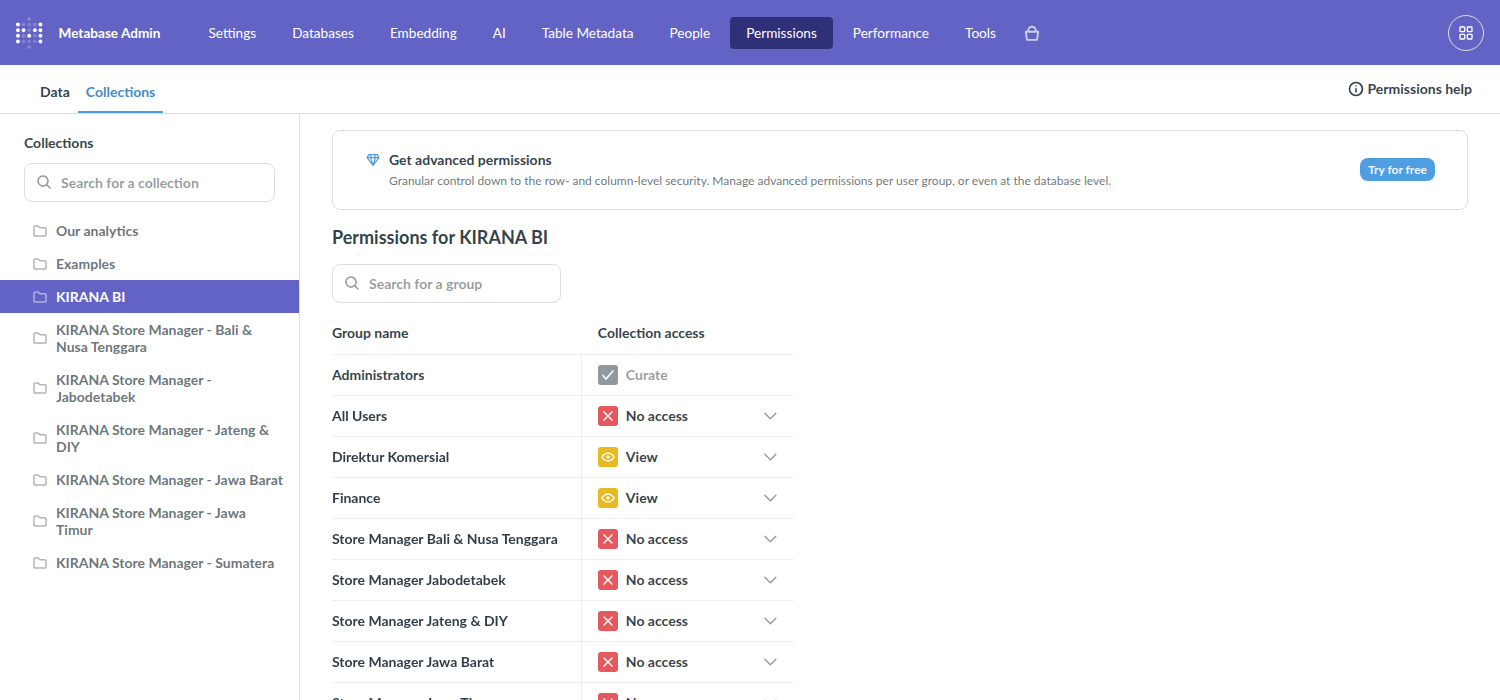
\includegraphics[keepaspectratio,alt={Izin koleksi KIRANA BI per grup}]{img/akses_izin_koleksi.png}}
\caption{Izin koleksi KIRANA BI per grup}
\end{figure}

\begin{figure}
\centering
\pandocbounded{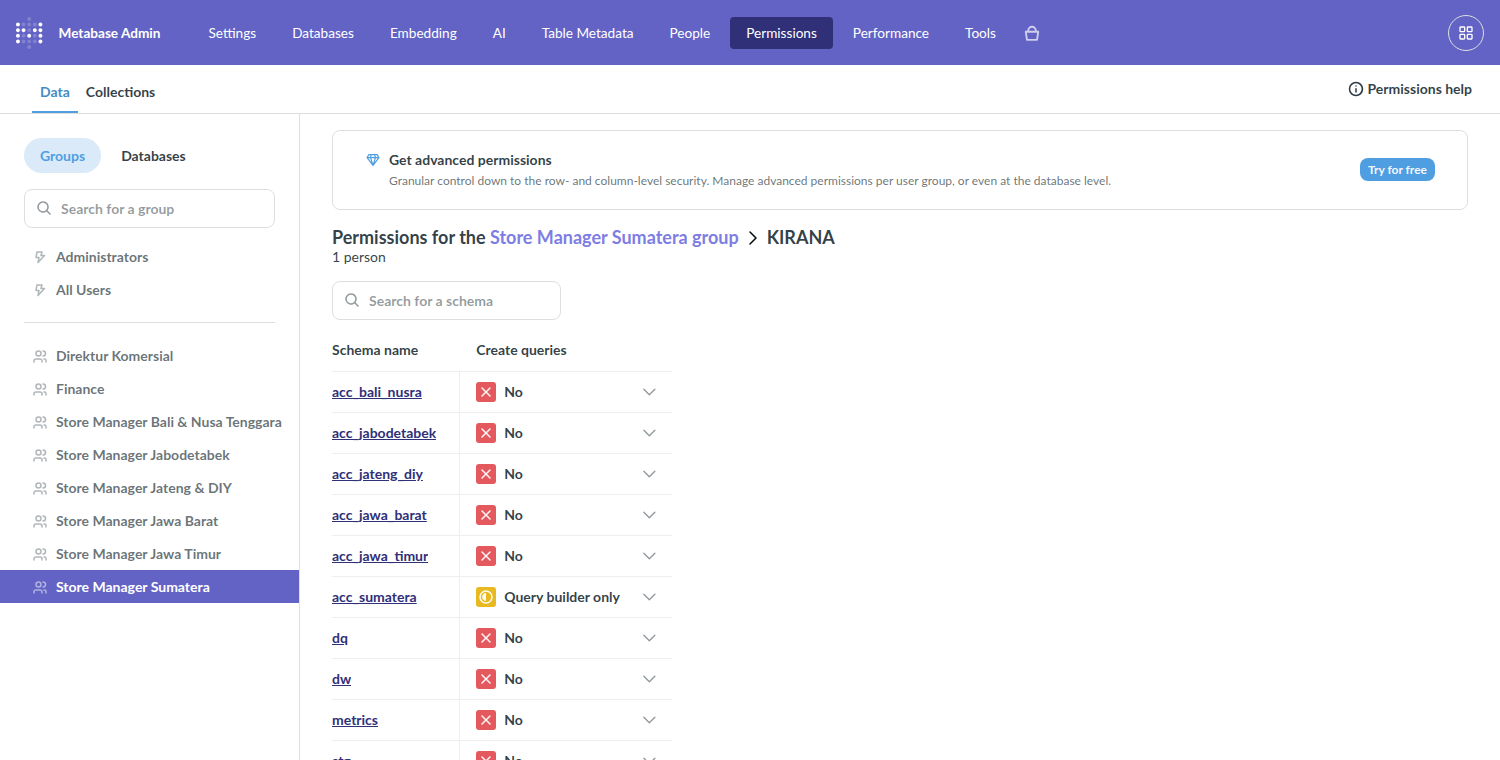
\includegraphics[keepaspectratio,alt={Izin data grup Store Manager Sumatera: hanya acc\_\allowbreak{}sumatera}]{img/akses_izin_data_sm_sumatera.png}}
\caption{Izin data grup Store Manager Sumatera: hanya acc\_\allowbreak{}sumatera}
\end{figure}

\begin{figure}
\centering
\pandocbounded{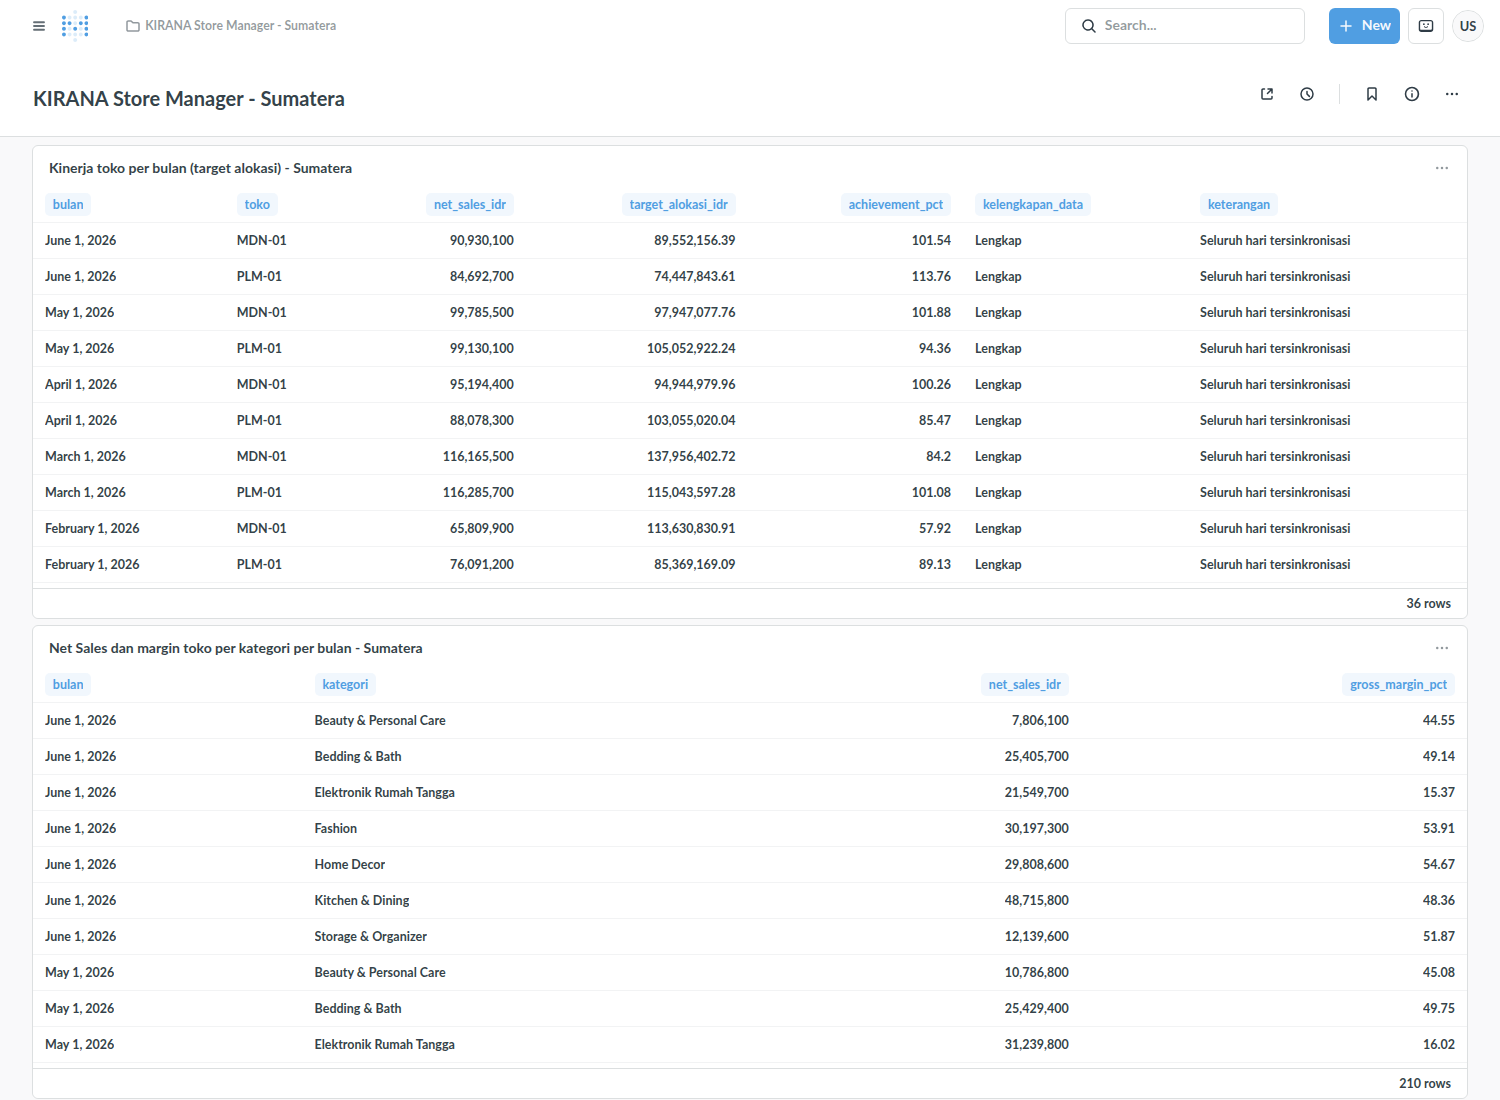
\includegraphics[keepaspectratio,alt={Dashboard yang dilihat pengguna Store Manager Sumatera}]{img/akses_dashboard_sm_sumatera.png}}
\caption{Dashboard yang dilihat pengguna Store Manager Sumatera}
\end{figure}

Pengaman lain \textbf{{[}Sudah{]}}: public sharing dimatikan (\texttt{MB\_\allowbreak{}ENABLE\_\allowbreak{}PUBLIC\_\allowbreak{}SHARING=false} di \href{https://github.com/titan2903/kirana-omnichannel-performance-intelligence/blob/master/compose.yaml}{\texttt{compose.yaml}}), tidak ada embedding, Metabase hanya mendengarkan \texttt{127.0.0.1}, koneksi DuckDB read-only, dan kredensial hanya lewat variabel lingkungan atau \texttt{.env} yang di-ignore.

\subsection{4. Lineage}\label{lineage}

\begin{figure}
\centering
\pandocbounded{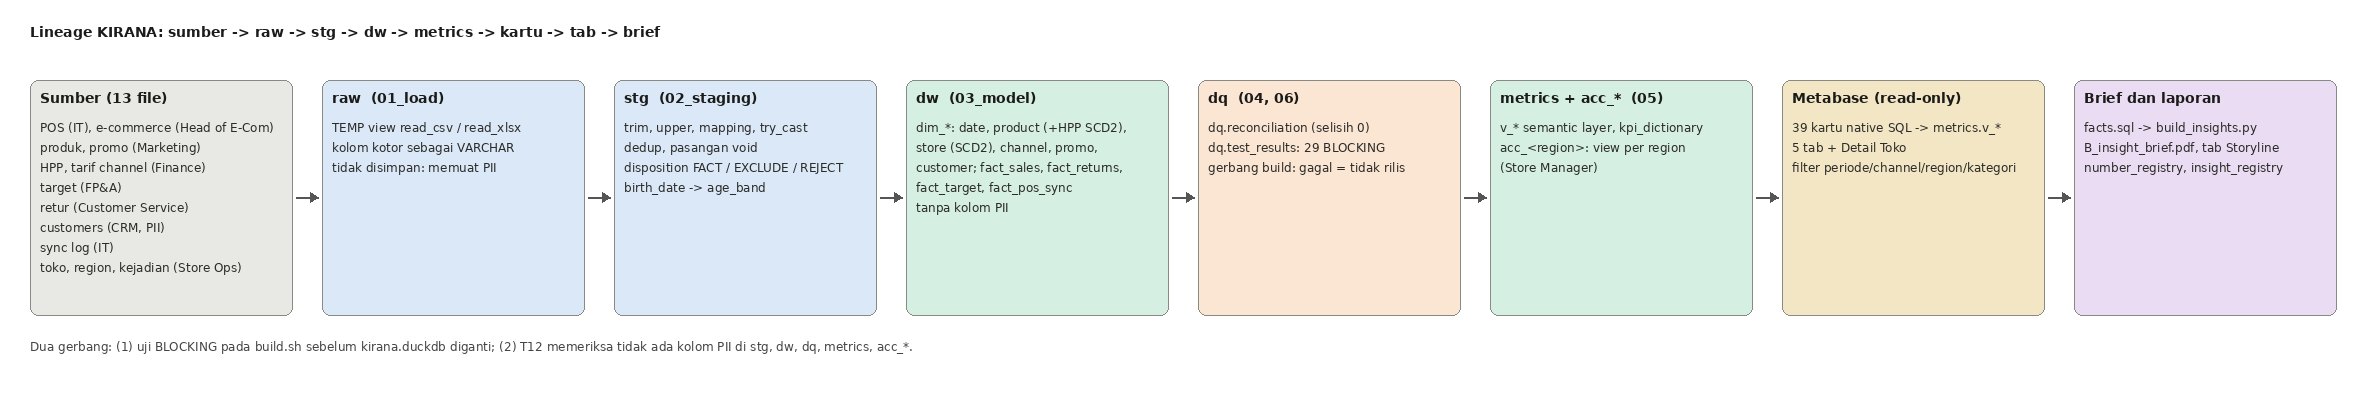
\includegraphics[keepaspectratio,alt={Lineage}]{img/lineage.png}}
\caption{Lineage}
\end{figure}

Sumber (\href{https://github.com/titan2903/kirana-omnichannel-performance-intelligence/blob/master/reports/img/lineage.drawio}{\texttt{reports/img/lineage.drawio}} dapat disunting di draw.io; dibuat ulang oleh \href{https://github.com/titan2903/kirana-omnichannel-performance-intelligence/blob/master/reports/img/build_lineage.py}{\texttt{reports/img/build\_\allowbreak{}lineage.py}}) \textbf{{[}Sudah{]}}. Rantai penuh: 13 file di \texttt{raw\_\allowbreak{}data/} → \texttt{raw} (TEMP view) → \texttt{stg} (\texttt{disposition} FACT / EXCLUDE / REJECT) → \texttt{dw} (star schema) → \texttt{dq} (rekonsiliasi, uji) → \texttt{metrics} dan \texttt{acc\_\allowbreak{}*} → 39 kartu Metabase (\href{https://github.com/titan2903/kirana-omnichannel-performance-intelligence/tree/master/dashboard/questions}{\texttt{dashboard/questions/*.sql}}) → 5 tab + Detail Toko → \texttt{B\_\allowbreak{}insight\_\allowbreak{}brief} (angka dari \href{https://github.com/titan2903/kirana-omnichannel-performance-intelligence/blob/master/reports/insights/facts.sql}{\texttt{reports/insights/facts.sql}}). Setiap angka di laporan dapat ditelusuri lewat Lampiran Number Registry dan \href{https://github.com/titan2903/kirana-omnichannel-performance-intelligence/blob/master/reports/insights/insight_registry.md}{\texttt{reports/insights/insight\_\allowbreak{}registry.md}} ke view dan filter sumbernya \textbf{{[}Sudah{]}}. Alat lineage otomatis (mis. dbt docs) adalah pengembangan \textbf{{[}Usulan{]}}.

\subsection{5. Refresh}\label{refresh}

{\def\LTcaptype{none} % do not increment counter
\begin{longtable}[]{@{}
  >{\raggedright\arraybackslash}p{(\linewidth - 4\tabcolsep) * \real{0.1100}}
  >{\raggedright\arraybackslash}p{(\linewidth - 4\tabcolsep) * \real{0.4800}}
  >{\raggedright\arraybackslash}p{(\linewidth - 4\tabcolsep) * \real{0.4100}}@{}}
\toprule\noalign{}
\begin{minipage}[b]{\linewidth}\raggedright
Aspek
\end{minipage} & \begin{minipage}[b]{\linewidth}\raggedright
Rancangan
\end{minipage} & \begin{minipage}[b]{\linewidth}\raggedright
Status
\end{minipage} \\
\midrule\noalign{}
\endhead
\bottomrule\noalign{}
\endlastfoot
Pemicu & Data POS tiba di pusat sekitar 01:00 sampai 01:49 (kolom \texttt{synced\_\allowbreak{}at}). Jadwalkan rebuild harian pukul \textbf{03:00} agar semua toko sudah mengirim & \textbf{{[}Usulan{]}} \\
Pelaksana & Tim Data \& Analytics (BI Analyst) menjalankan satu perintah, \href{https://github.com/titan2903/kirana-omnichannel-performance-intelligence/blob/master/scripts/build.sh}{\texttt{bash\ scripts/build.sh}}; bisa dijadwalkan lewat cron & Skrip \textbf{{[}Sudah{]}}, jadwal \textbf{{[}Usulan{]}} \\
Urutan & (1) \texttt{docker\ compose\ stop\ metabase}, (2) \href{https://github.com/titan2903/kirana-omnichannel-performance-intelligence/blob/master/scripts/build.sh}{\texttt{bash\ scripts/build.sh}} (build ke berkas sementara, menukar \texttt{kirana.duckdb} hanya bila uji BLOCKING lolos), (3) \texttt{docker\ compose\ start\ metabase} dan sync schema & Urutan \textbf{{[}Sudah{]}} dan didokumentasikan di README \\
Idempoten & Dua kali build menghasilkan 62 objek identik (\href{https://github.com/titan2903/kirana-omnichannel-performance-intelligence/blob/master/scripts/idempotency_check.sh}{\texttt{idempotency\_\allowbreak{}check.sh}}) & \textbf{{[}Sudah{]}} \\
Kesegaran & Kartu \texttt{kesegaran\_\allowbreak{}data} menampilkan tanggal data terakhir (30 Jun 2026), persentase sync berhasil, toko-hari gagal & \textbf{{[}Sudah{]}} \\
\end{longtable}
}

\subsection{6. Monitoring}\label{monitoring}

{\def\LTcaptype{none} % do not increment counter
\begin{longtable}[]{@{}
  >{\raggedright\arraybackslash}p{(\linewidth - 4\tabcolsep) * \real{0.3400}}
  >{\raggedright\arraybackslash}p{(\linewidth - 4\tabcolsep) * \real{0.3700}}
  >{\raggedright\arraybackslash}p{(\linewidth - 4\tabcolsep) * \real{0.2900}}@{}}
\toprule\noalign{}
\begin{minipage}[b]{\linewidth}\raggedright
Pemantauan
\end{minipage} & \begin{minipage}[b]{\linewidth}\raggedright
Ambang dan tindakan
\end{minipage} & \begin{minipage}[b]{\linewidth}\raggedright
Status
\end{minipage} \\
\midrule\noalign{}
\endhead
\bottomrule\noalign{}
\endlastfoot
Uji BLOCKING (29 uji) & Satu uji gagal menghentikan build; \texttt{kirana.duckdb} lama tetap dipakai & \textbf{{[}Sudah{]}} \\
Uji WARNING (14 uji, 3 temuan dikenal: T21, T22, T29) & Dicatat; temuan baru ditinjau pemilik sumber & \textbf{{[}Sudah{]}} \\
Rekonsiliasi raw → fakta & Selisih ≠ 0 membuat T10 dan T11 gagal & \textbf{{[}Sudah{]}} \\
Uji mutasi & 39 cacat disuntik, semua terdeteksi; jalankan setelah mengubah model & \textbf{{[}Sudah{]}} \\
Sync POS FAILED & Notifikasi ke IT bila ada toko-hari FAILED atau lebih dari 1 hari berturut-turut; dashboard menandai toko sebagai data tidak lengkap & Penanda \textbf{{[}Sudah{]}}; notifikasi \textbf{{[}Usulan{]}} \\
Freshness & Peringatan bila tanggal data terakhir lebih dari 2 hari dari tanggal rebuild & \textbf{{[}Usulan{]}} \\
Log akses Metabase & Tinjau bulanan siapa membuka dashboard dan perubahan grup & \textbf{{[}Usulan{]}} \\
\end{longtable}
}

\subsection{7. Retensi (semuanya usulan dan asumsi, menunggu kebijakan perusahaan)}\label{retensi-semuanya-usulan-dan-asumsi-menunggu-kebijakan-perusahaan}

{\def\LTcaptype{none} % do not increment counter
\begin{longtable}[]{@{}
  >{\raggedright\arraybackslash}p{(\linewidth - 4\tabcolsep) * \real{0.2222}}
  >{\raggedright\arraybackslash}p{(\linewidth - 4\tabcolsep) * \real{0.3939}}
  >{\raggedright\arraybackslash}p{(\linewidth - 4\tabcolsep) * \real{0.3838}}@{}}
\toprule\noalign{}
\begin{minipage}[b]{\linewidth}\raggedright
Data
\end{minipage} & \begin{minipage}[b]{\linewidth}\raggedright
Usulan retensi
\end{minipage} & \begin{minipage}[b]{\linewidth}\raggedright
Alasan
\end{minipage} \\
\midrule\noalign{}
\endhead
\bottomrule\noalign{}
\endlastfoot
Data mentah transaksi & Minimal 24 bulan online, lalu arsip; paket ini mencakup 30 bulan & Perbandingan YoY dan evaluasi target butuh dua tahun lebih \\
\texttt{customers.csv} (PII) & Dibatasi pada CRM; akses di luar CRM tidak diberikan; hapus atau anonimkan sesuai permintaan penghapusan dan kebijakan privasi & Prinsip minimisasi data \\
\texttt{kirana.duckdb} & Dapat dibangun ulang; simpan tiga versi terakhir & Bukan sumber kebenaran, \texttt{raw\_\allowbreak{}data/} adalah sumbernya \\
Log akses Metabase & 12 bulan & Audit \\
Hasil uji (\texttt{dq.test\_\allowbreak{}results}) & Disimpan per build & Bukti kualitas \\
\end{longtable}
}

\clearpage
% ======== number_registry ========
\section{Number Registry}\label{number-registry}

Dihasilkan otomatis oleh \href{https://github.com/titan2903/kirana-omnichannel-performance-intelligence/blob/master/scripts/export_reports.sh}{\texttt{scripts/export\_\allowbreak{}reports.sh}} dari \texttt{kirana.duckdb}. Setiap angka di insight brief dan laporan harus berasal dari sini
(atau dari kartu Metabase yang membaca view yang sama). Periode: FY2024 = Jan--Des 2024, FY2025 = Jan--Des 2025, H1 2026 = Jan--Jun 2026.
Rupiah, tanpa pajak. Rasio dihitung ulang dari pembilang/penyebut. Data sampai: 30 Jun 2026.

\subsection{1. Net Sales per channel dan periode}\label{net-sales-per-channel-dan-periode}

\emph{View: \texttt{metrics.v\_\allowbreak{}sales\_\allowbreak{}monthly}. Filter: periode. Termasuk B2B bulk.}

{\def\LTcaptype{none} % do not increment counter
\begin{longtable}[]{@{}
  >{\raggedright\arraybackslash}p{(\linewidth - 6\tabcolsep) * \real{0.1667}}
  >{\raggedright\arraybackslash}p{(\linewidth - 6\tabcolsep) * \real{0.2451}}
  >{\raggedleft\arraybackslash}p{(\linewidth - 6\tabcolsep) * \real{0.2843}}
  >{\raggedleft\arraybackslash}p{(\linewidth - 6\tabcolsep) * \real{0.3039}}@{}}
\toprule\noalign{}
\begin{minipage}[b]{\linewidth}\raggedright
periode
\end{minipage} & \begin{minipage}[b]{\linewidth}\raggedright
channel
\end{minipage} & \begin{minipage}[b]{\linewidth}\raggedleft
net\_\allowbreak{}sales\_\allowbreak{}idr
\end{minipage} & \begin{minipage}[b]{\linewidth}\raggedleft
kontribusi\_\allowbreak{}pct
\end{minipage} \\
\midrule\noalign{}
\endhead
\bottomrule\noalign{}
\endlastfoot
FY2024 & Marketplace & 6564843100 & 17.5 \\
FY2024 & Mobile App & 3949287900 & 10.5 \\
FY2024 & Store & 23585615400 & 62.7 \\
FY2024 & Website & 3519832900 & 9.4 \\
FY2025 & Marketplace & 9293547000 & 21.1 \\
FY2025 & Mobile App & 6601860400 & 15.0 \\
FY2025 & Store & 25234099400 & 57.4 \\
FY2025 & Website & 2827730500 & 6.4 \\
H1 2026 & Marketplace & 5865550500 & 23.3 \\
H1 2026 & Mobile App & 4702395100 & 18.7 \\
H1 2026 & Store & 13404994900 & 53.2 \\
H1 2026 & Website & 1237537600 & 4.9 \\
\end{longtable}
}

\subsection{2. Achievement vs Target per channel}\label{achievement-vs-target-per-channel}

\emph{View: \texttt{metrics.v\_\allowbreak{}target\_\allowbreak{}achievement}. Filter: periode FY2025 dan H1 2026 (2024 tidak punya target).}

{\def\LTcaptype{none} % do not increment counter
\begin{longtable}[]{@{}
  >{\raggedright\arraybackslash}p{(\linewidth - 10\tabcolsep) * \real{0.1176}}
  >{\raggedright\arraybackslash}p{(\linewidth - 10\tabcolsep) * \real{0.1667}}
  >{\raggedleft\arraybackslash}p{(\linewidth - 10\tabcolsep) * \real{0.2059}}
  >{\raggedleft\arraybackslash}p{(\linewidth - 10\tabcolsep) * \real{0.1765}}
  >{\raggedleft\arraybackslash}p{(\linewidth - 10\tabcolsep) * \real{0.2255}}
  >{\raggedright\arraybackslash}p{(\linewidth - 10\tabcolsep) * \real{0.1078}}@{}}
\toprule\noalign{}
\begin{minipage}[b]{\linewidth}\raggedright
periode
\end{minipage} & \begin{minipage}[b]{\linewidth}\raggedright
channel
\end{minipage} & \begin{minipage}[b]{\linewidth}\raggedleft
net\_\allowbreak{}sales\_\allowbreak{}idr
\end{minipage} & \begin{minipage}[b]{\linewidth}\raggedleft
target\_\allowbreak{}idr
\end{minipage} & \begin{minipage}[b]{\linewidth}\raggedleft
achievement\_\allowbreak{}pct
\end{minipage} & \begin{minipage}[b]{\linewidth}\raggedright
status
\end{minipage} \\
\midrule\noalign{}
\endhead
\bottomrule\noalign{}
\endlastfoot
FY2025 & Marketplace & 9293547000 & 8525000000 & 109.0 & Hijau \\
FY2025 & Mobile App & 6601860400 & 5542000000 & 119.1 & Hijau \\
FY2025 & Store & 25234099400 & 26391000000 & 95.6 & Kuning \\
FY2025 & Website & 2827730500 & 3723000000 & 76.0 & Merah \\
H1 2026 & Marketplace & 5865550500 & 4601000000 & 127.5 & Hijau \\
H1 2026 & Mobile App & 4702395100 & 3782000000 & 124.3 & Hijau \\
H1 2026 & Store & 13404994900 & 14022000000 & 95.6 & Kuning \\
H1 2026 & Website & 1237537600 & 1415000000 & 87.5 & Merah \\
\end{longtable}
}

\subsection{3. Achievement Store per region}\label{achievement-store-per-region}

\emph{View: \texttt{metrics.v\_\allowbreak{}target\_\allowbreak{}achievement} (channel Store, region dasar target \texttt{region\_\allowbreak{}target\_\allowbreak{}basis} = region awal tahun).}

{\def\LTcaptype{none} % do not increment counter
\begin{longtable}[]{@{}
  >{\raggedright\arraybackslash}p{(\linewidth - 10\tabcolsep) * \real{0.1068}}
  >{\raggedright\arraybackslash}p{(\linewidth - 10\tabcolsep) * \real{0.2524}}
  >{\raggedleft\arraybackslash}p{(\linewidth - 10\tabcolsep) * \real{0.1845}}
  >{\raggedleft\arraybackslash}p{(\linewidth - 10\tabcolsep) * \real{0.1553}}
  >{\raggedleft\arraybackslash}p{(\linewidth - 10\tabcolsep) * \real{0.2039}}
  >{\raggedright\arraybackslash}p{(\linewidth - 10\tabcolsep) * \real{0.0971}}@{}}
\toprule\noalign{}
\begin{minipage}[b]{\linewidth}\raggedright
periode
\end{minipage} & \begin{minipage}[b]{\linewidth}\raggedright
region
\end{minipage} & \begin{minipage}[b]{\linewidth}\raggedleft
net\_\allowbreak{}sales\_\allowbreak{}idr
\end{minipage} & \begin{minipage}[b]{\linewidth}\raggedleft
target\_\allowbreak{}idr
\end{minipage} & \begin{minipage}[b]{\linewidth}\raggedleft
achievement\_\allowbreak{}pct
\end{minipage} & \begin{minipage}[b]{\linewidth}\raggedright
status
\end{minipage} \\
\midrule\noalign{}
\endhead
\bottomrule\noalign{}
\endlastfoot
FY2025 & Bali \& Nusa Tenggara & 1124506000 & 1239000000 & 90.8 & Kuning \\
FY2025 & Jabodetabek & 9494637900 & 9932000000 & 95.6 & Kuning \\
FY2025 & Jateng \& DIY & 3545477900 & 3500000000 & 101.3 & Hijau \\
FY2025 & Jawa Barat & 4465127100 & 4430000000 & 100.8 & Hijau \\
FY2025 & Jawa Timur & 4382882600 & 4729000000 & 92.7 & Kuning \\
FY2025 & Sumatera & 2221467900 & 2561000000 & 86.7 & Merah \\
H1 2026 & Bali \& Nusa Tenggara & 755030500 & 782000000 & 96.6 & Kuning \\
H1 2026 & Jabodetabek & 5679016700 & 5872000000 & 96.7 & Kuning \\
H1 2026 & Jateng \& DIY & 1777878900 & 1935000000 & 91.9 & Kuning \\
H1 2026 & Jawa Barat & 1653486600 & 1726000000 & 95.8 & Kuning \\
H1 2026 & Jawa Timur & 2439007800 & 2470000000 & 98.7 & Kuning \\
H1 2026 & Sumatera & 1100574400 & 1237000000 & 89.0 & Merah \\
\end{longtable}
}

\subsection{4. Achievement per toko (target ALOKASI, asumsi)}\label{achievement-per-toko-target-alokasi-asumsi}

\emph{View: \texttt{metrics.v\_\allowbreak{}store\_\allowbreak{}target\_\allowbreak{}alloc}. Hanya toko dengan achievement terendah per periode; daftar lengkap di view.}

{\def\LTcaptype{none} % do not increment counter
\begin{longtable}[]{@{}
  >{\raggedright\arraybackslash}p{(\linewidth - 10\tabcolsep) * \real{0.0980}}
  >{\raggedright\arraybackslash}p{(\linewidth - 10\tabcolsep) * \real{0.0882}}
  >{\raggedright\arraybackslash}p{(\linewidth - 10\tabcolsep) * \real{0.2353}}
  >{\raggedleft\arraybackslash}p{(\linewidth - 10\tabcolsep) * \real{0.1765}}
  >{\raggedleft\arraybackslash}p{(\linewidth - 10\tabcolsep) * \real{0.2059}}
  >{\raggedleft\arraybackslash}p{(\linewidth - 10\tabcolsep) * \real{0.1961}}@{}}
\toprule\noalign{}
\begin{minipage}[b]{\linewidth}\raggedright
periode
\end{minipage} & \begin{minipage}[b]{\linewidth}\raggedright
toko
\end{minipage} & \begin{minipage}[b]{\linewidth}\raggedright
region
\end{minipage} & \begin{minipage}[b]{\linewidth}\raggedleft
net\_\allowbreak{}sales\_\allowbreak{}idr
\end{minipage} & \begin{minipage}[b]{\linewidth}\raggedleft
store\_\allowbreak{}target\_\allowbreak{}idr
\end{minipage} & \begin{minipage}[b]{\linewidth}\raggedleft
achievement\_\allowbreak{}pct
\end{minipage} \\
\midrule\noalign{}
\endhead
\bottomrule\noalign{}
\endlastfoot
FY2025 & MDN-01 & Sumatera & 1154377400 & 1455754782 & 79.3 \\
FY2025 & SBY-01 & Jawa Timur & 1995235000 & 2241752328 & 89.0 \\
FY2025 & JKT-03 & Jabodetabek & 1506758500 & 1670893994 & 90.2 \\
FY2025 & DPK-01 & Jabodetabek & 911142500 & 1009850993 & 90.2 \\
FY2025 & DPS-01 & Bali \& Nusa Tenggara & 1124506000 & 1239000000 & 90.8 \\
H1 2026 & MDN-01 & Sumatera & 544980300 & 652367619 & 83.5 \\
H1 2026 & SBY-02 & Jawa Timur & 629045100 & 716189392 & 87.8 \\
H1 2026 & MLG-01 & Jawa Timur & 534782500 & 608241365 & 87.9 \\
H1 2026 & SOL-01 & Jateng \& DIY & 441268900 & 490862178 & 89.9 \\
H1 2026 & YGY-01 & Jateng \& DIY & 637043000 & 700466062 & 90.9 \\
\end{longtable}
}

\subsection{5. Gross Margin \% dan Contribution Margin \% per channel}\label{gross-margin-dan-contribution-margin-per-channel}

\emph{View: \texttt{metrics.v\_\allowbreak{}margin\_\allowbreak{}vs\_\allowbreak{}target}. GM target dari FP\&A; CM target = Target GM - tarif channel (ASUMSI).}

{\def\LTcaptype{none} % do not increment counter
\begin{longtable}[]{@{}
  >{\raggedright\arraybackslash}p{(\linewidth - 8\tabcolsep) * \real{0.1667}}
  >{\raggedright\arraybackslash}p{(\linewidth - 8\tabcolsep) * \real{0.2451}}
  >{\raggedleft\arraybackslash}p{(\linewidth - 8\tabcolsep) * \real{0.1569}}
  >{\raggedright\arraybackslash}p{(\linewidth - 8\tabcolsep) * \real{0.2745}}
  >{\raggedleft\arraybackslash}p{(\linewidth - 8\tabcolsep) * \real{0.1569}}@{}}
\toprule\noalign{}
\begin{minipage}[b]{\linewidth}\raggedright
periode
\end{minipage} & \begin{minipage}[b]{\linewidth}\raggedright
channel
\end{minipage} & \begin{minipage}[b]{\linewidth}\raggedleft
gm\_\allowbreak{}pct
\end{minipage} & \begin{minipage}[b]{\linewidth}\raggedright
target\_\allowbreak{}gm\_\allowbreak{}pct
\end{minipage} & \begin{minipage}[b]{\linewidth}\raggedleft
cm\_\allowbreak{}pct
\end{minipage} \\
\midrule\noalign{}
\endhead
\bottomrule\noalign{}
\endlastfoot
FY2024 & Marketplace & 43.88 & NULL & 34.88 \\
FY2024 & Mobile App & 44.57 & NULL & 42.37 \\
FY2024 & Store & 46.92 & NULL & 46.22 \\
FY2024 & Website & 46.54 & NULL & 44.34 \\
FY2025 & Marketplace & 41.84 & 42.0 & 30.87 \\
FY2025 & Mobile App & 42.07 & 43.0 & 39.87 \\
FY2025 & Store & 45.7 & 46.0 & 45.0 \\
FY2025 & Website & 45.46 & 45.0 & 43.26 \\
H1 2026 & Marketplace & 42.08 & 42.0 & 30.58 \\
H1 2026 & Mobile App & 40.48 & 43.0 & 38.28 \\
H1 2026 & Store & 44.29 & 46.0 & 43.59 \\
H1 2026 & Website & 43.89 & 45.0 & 41.69 \\
\end{longtable}
}

\subsection{6. Gross Margin \% total per periode (efek SCD HPP)}\label{gross-margin-total-per-periode-efek-scd-hpp}

\emph{View: \texttt{metrics.v\_\allowbreak{}sales\_\allowbreak{}monthly}. Pembanding dengan HPP terkini ada di \href{https://github.com/titan2903/kirana-omnichannel-performance-intelligence/blob/master/sql/analysis/scd_impact.sql}{\texttt{sql/analysis/scd\_\allowbreak{}impact.sql}}.}

{\def\LTcaptype{none} % do not increment counter
\begin{longtable}[]{@{}
  >{\raggedright\arraybackslash}p{(\linewidth - 6\tabcolsep) * \real{0.2233}}
  >{\raggedleft\arraybackslash}p{(\linewidth - 6\tabcolsep) * \real{0.3689}}
  >{\raggedleft\arraybackslash}p{(\linewidth - 6\tabcolsep) * \real{0.2039}}
  >{\raggedleft\arraybackslash}p{(\linewidth - 6\tabcolsep) * \real{0.2039}}@{}}
\toprule\noalign{}
\begin{minipage}[b]{\linewidth}\raggedright
periode
\end{minipage} & \begin{minipage}[b]{\linewidth}\raggedleft
net\_\allowbreak{}sales\_\allowbreak{}idr
\end{minipage} & \begin{minipage}[b]{\linewidth}\raggedleft
gm\_\allowbreak{}pct
\end{minipage} & \begin{minipage}[b]{\linewidth}\raggedleft
cm\_\allowbreak{}pct
\end{minipage} \\
\midrule\noalign{}
\endhead
\bottomrule\noalign{}
\endlastfoot
FY2024 & 37619579300 & 46.11 & 43.66 \\
FY2025 & 43957237300 & 44.32 & 41.13 \\
H1 2026 & 25210478100 & 43.05 & 39.48 \\
\end{longtable}
}

\subsection{7. Jumlah Transaksi dan AOV per channel}\label{jumlah-transaksi-dan-aov-per-channel}

\emph{View: \texttt{metrics.v\_\allowbreak{}txn\_\allowbreak{}monthly}. AOV = SUM(net\_\allowbreak{}sales\_\allowbreak{}idr) / SUM(transactions).}

{\def\LTcaptype{none} % do not increment counter
\begin{longtable}[]{@{}
  >{\raggedright\arraybackslash}p{(\linewidth - 6\tabcolsep) * \real{0.2079}}
  >{\raggedright\arraybackslash}p{(\linewidth - 6\tabcolsep) * \real{0.3069}}
  >{\raggedleft\arraybackslash}p{(\linewidth - 6\tabcolsep) * \real{0.2673}}
  >{\raggedleft\arraybackslash}p{(\linewidth - 6\tabcolsep) * \real{0.2178}}@{}}
\toprule\noalign{}
\begin{minipage}[b]{\linewidth}\raggedright
periode
\end{minipage} & \begin{minipage}[b]{\linewidth}\raggedright
channel
\end{minipage} & \begin{minipage}[b]{\linewidth}\raggedleft
transaksi
\end{minipage} & \begin{minipage}[b]{\linewidth}\raggedleft
aov\_\allowbreak{}idr
\end{minipage} \\
\midrule\noalign{}
\endhead
\bottomrule\noalign{}
\endlastfoot
FY2024 & Marketplace & 19984 & 328505 \\
FY2024 & Mobile App & 11679 & 338153 \\
FY2024 & Store & 54720 & 431024 \\
FY2024 & Website & 10254 & 343264 \\
FY2025 & Marketplace & 28133 & 330343 \\
FY2025 & Mobile App & 19418 & 339987 \\
FY2025 & Store & 58480 & 431500 \\
FY2025 & Website & 8336 & 339219 \\
H1 2026 & Marketplace & 17116 & 342694 \\
H1 2026 & Mobile App & 13649 & 344523 \\
H1 2026 & Store & 30569 & 438516 \\
H1 2026 & Website & 3468 & 356845 \\
\end{longtable}
}

\subsection{8. Return Rate per channel}\label{return-rate-per-channel}

\emph{View: \texttt{metrics.v\_\allowbreak{}return\_\allowbreak{}rate\_\allowbreak{}monthly}. Rate Rp = SUM(refund\_\allowbreak{}idr) / SUM(net\_\allowbreak{}sales\_\allowbreak{}idr); retur menurut tanggal retur.}

{\def\LTcaptype{none} % do not increment counter
\begin{longtable}[]{@{}
  >{\raggedright\arraybackslash}p{(\linewidth - 8\tabcolsep) * \real{0.1262}}
  >{\raggedright\arraybackslash}p{(\linewidth - 8\tabcolsep) * \real{0.1748}}
  >{\raggedleft\arraybackslash}p{(\linewidth - 8\tabcolsep) * \real{0.1748}}
  >{\raggedleft\arraybackslash}p{(\linewidth - 8\tabcolsep) * \real{0.2330}}
  >{\raggedleft\arraybackslash}p{(\linewidth - 8\tabcolsep) * \real{0.2913}}@{}}
\toprule\noalign{}
\begin{minipage}[b]{\linewidth}\raggedright
periode
\end{minipage} & \begin{minipage}[b]{\linewidth}\raggedright
channel
\end{minipage} & \begin{minipage}[b]{\linewidth}\raggedleft
refund\_\allowbreak{}idr
\end{minipage} & \begin{minipage}[b]{\linewidth}\raggedleft
return\_\allowbreak{}rate\_\allowbreak{}pct
\end{minipage} & \begin{minipage}[b]{\linewidth}\raggedleft
return\_\allowbreak{}rate\_\allowbreak{}unit\_\allowbreak{}pct
\end{minipage} \\
\midrule\noalign{}
\endhead
\bottomrule\noalign{}
\endlastfoot
FY2024 & Marketplace & 408768500 & 6.23 & 5.92 \\
FY2024 & Mobile App & 195843600 & 4.96 & 5.31 \\
FY2024 & Store & 426032200 & 1.81 & 1.77 \\
FY2024 & Website & 144355200 & 4.1 & 4.42 \\
FY2025 & Marketplace & 605383700 & 6.51 & 6.24 \\
FY2025 & Mobile App & 342923100 & 5.19 & 5.44 \\
FY2025 & Store & 508220200 & 2.01 & 1.98 \\
FY2025 & Website & 129191600 & 4.57 & 4.67 \\
H1 2026 & Marketplace & 373681500 & 6.37 & 6.29 \\
H1 2026 & Mobile App & 240793100 & 5.12 & 5.39 \\
H1 2026 & Store & 265847200 & 1.98 & 2.04 \\
H1 2026 & Website & 60787400 & 4.91 & 4.62 \\
\end{longtable}
}

\subsection{9. Alasan retur (seluruh periode)}\label{alasan-retur-seluruh-periode}

\emph{View: \texttt{metrics.v\_\allowbreak{}return\_\allowbreak{}reason\_\allowbreak{}monthly}.}

{\def\LTcaptype{none} % do not increment counter
\begin{longtable}[]{@{}
  >{\raggedright\arraybackslash}p{(\linewidth - 6\tabcolsep) * \real{0.3786}}
  >{\raggedleft\arraybackslash}p{(\linewidth - 6\tabcolsep) * \real{0.1165}}
  >{\raggedleft\arraybackslash}p{(\linewidth - 6\tabcolsep) * \real{0.2039}}
  >{\raggedleft\arraybackslash}p{(\linewidth - 6\tabcolsep) * \real{0.3010}}@{}}
\toprule\noalign{}
\begin{minipage}[b]{\linewidth}\raggedright
alasan
\end{minipage} & \begin{minipage}[b]{\linewidth}\raggedleft
retur
\end{minipage} & \begin{minipage}[b]{\linewidth}\raggedleft
refund\_\allowbreak{}idr
\end{minipage} & \begin{minipage}[b]{\linewidth}\raggedleft
pangsa\_\allowbreak{}refund\_\allowbreak{}pct
\end{minipage} \\
\midrule\noalign{}
\endhead
\bottomrule\noalign{}
\endlastfoot
Barang cacat & 3539 & 855415400 & 23.1 \\
Ukuran tidak sesuai & 4806 & 855279500 & 23.1 \\
Berubah pikiran & 3001 & 571854800 & 15.4 \\
Rusak saat pengiriman & 2434 & 563880600 & 15.2 \\
Tidak sesuai deskripsi & 1925 & 424429300 & 11.5 \\
Warna berbeda dari foto & 1545 & 281566600 & 7.6 \\
Salah kirim & 839 & 149401100 & 4.0 \\
\end{longtable}
}

\subsection{10. Active Members dan Repeat Rate}\label{active-members-dan-repeat-rate}

\emph{View: \texttt{metrics.v\_\allowbreak{}members\_\allowbreak{}period} (period\_\allowbreak{}type Tahun untuk FY2024 dan FY2025, Semester untuk H1 2025 dan H1 2026). Struk B2B dikecualikan. Bandingkan hanya periode sama panjang: H1 2026 dengan H1 2025, bukan dengan FY.}

{\def\LTcaptype{none} % do not increment counter
\begin{longtable}[]{@{}
  >{\raggedright\arraybackslash}p{(\linewidth - 8\tabcolsep) * \real{0.1250}}
  >{\raggedright\arraybackslash}p{(\linewidth - 8\tabcolsep) * \real{0.2019}}
  >{\raggedleft\arraybackslash}p{(\linewidth - 8\tabcolsep) * \real{0.2212}}
  >{\raggedleft\arraybackslash}p{(\linewidth - 8\tabcolsep) * \real{0.2212}}
  >{\raggedleft\arraybackslash}p{(\linewidth - 8\tabcolsep) * \real{0.2308}}@{}}
\toprule\noalign{}
\begin{minipage}[b]{\linewidth}\raggedright
periode
\end{minipage} & \begin{minipage}[b]{\linewidth}\raggedright
channel
\end{minipage} & \begin{minipage}[b]{\linewidth}\raggedleft
active\_\allowbreak{}members
\end{minipage} & \begin{minipage}[b]{\linewidth}\raggedleft
repeat\_\allowbreak{}members
\end{minipage} & \begin{minipage}[b]{\linewidth}\raggedleft
repeat\_\allowbreak{}rate\_\allowbreak{}pct
\end{minipage} \\
\midrule\noalign{}
\endhead
\bottomrule\noalign{}
\endlastfoot
FY2024 & Marketplace & 13049 & 4184 & 32.06 \\
FY2024 & Mobile App & 8820 & 2003 & 22.71 \\
FY2024 & Semua channel & 30450 & 18505 & 60.77 \\
FY2024 & Store & 19474 & 7511 & 38.57 \\
FY2024 & Website & 7968 & 1627 & 20.42 \\
FY2025 & Marketplace & 16307 & 6257 & 38.37 \\
FY2025 & Mobile App & 12781 & 3973 & 31.09 \\
FY2025 & Semua channel & 32707 & 21631 & 66.14 \\
FY2025 & Store & 20713 & 8213 & 39.65 \\
FY2025 & Website & 6756 & 1194 & 17.67 \\
H1 2025 & Marketplace & 9011 & 2066 & 22.93 \\
H1 2025 & Mobile App & 6767 & 1275 & 18.84 \\
H1 2025 & Semua channel & 23255 & 10068 & 43.29 \\
H1 2025 & Store & 12707 & 2741 & 21.57 \\
H1 2025 & Website & 3829 & 408 & 10.66 \\
H1 2026 & Marketplace & 11637 & 3381 & 29.05 \\
H1 2026 & Mobile App & 9993 & 2456 & 24.58 \\
H1 2026 & Semua channel & 25618 & 12837 & 50.11 \\
H1 2026 & Store & 13122 & 3144 & 23.96 \\
H1 2026 & Website & 3140 & 286 & 9.11 \\
\end{longtable}
}

\subsection{11. Cancellation Rate (online) dan Void Rate (POS)}\label{cancellation-rate-online-dan-void-rate-pos}

\emph{View: \texttt{metrics.v\_\allowbreak{}cancellation\_\allowbreak{}void\_\allowbreak{}monthly}.}

{\def\LTcaptype{none} % do not increment counter
\begin{longtable}[]{@{}
  >{\raggedright\arraybackslash}p{(\linewidth - 4\tabcolsep) * \real{0.1569}}
  >{\raggedleft\arraybackslash}p{(\linewidth - 4\tabcolsep) * \real{0.5000}}
  >{\raggedleft\arraybackslash}p{(\linewidth - 4\tabcolsep) * \real{0.3431}}@{}}
\toprule\noalign{}
\begin{minipage}[b]{\linewidth}\raggedright
periode
\end{minipage} & \begin{minipage}[b]{\linewidth}\raggedleft
cancellation\_\allowbreak{}rate\_\allowbreak{}online\_\allowbreak{}pct
\end{minipage} & \begin{minipage}[b]{\linewidth}\raggedleft
void\_\allowbreak{}rate\_\allowbreak{}pos\_\allowbreak{}pct
\end{minipage} \\
\midrule\noalign{}
\endhead
\bottomrule\noalign{}
\endlastfoot
FY2024 & 5.95 & 0.63 \\
FY2025 & 6.16 & 0.67 \\
H1 2026 & 6.09 & 0.66 \\
\end{longtable}
}

\subsection{12. Promo: Lift dan dampak margin per jenis}\label{promo-lift-dan-dampak-margin-per-jenis}

\emph{View: \texttt{metrics.v\_\allowbreak{}promo\_\allowbreak{}performance}. Lift dan perubahan GM per jenis = rasio gabungan (jumlah pembilang / jumlah penyebut), sama dengan kartu Metabase dan brief; min/maks = rentang lift per kode; nilai Rupiah dijumlahkan. Baseline simetris +/-1 sampai 4 minggu.}

{\def\LTcaptype{none} % do not increment counter
\begin{longtable}[]{@{}
  >{\raggedright\arraybackslash}p{(\linewidth - 22\tabcolsep) * \real{0.0600}}
  >{\raggedleft\arraybackslash}p{(\linewidth - 22\tabcolsep) * \real{0.0300}}
  >{\raggedleft\arraybackslash}p{(\linewidth - 22\tabcolsep) * \real{0.0700}}
  >{\raggedleft\arraybackslash}p{(\linewidth - 22\tabcolsep) * \real{0.0700}}
  >{\raggedleft\arraybackslash}p{(\linewidth - 22\tabcolsep) * \real{0.0750}}
  >{\raggedleft\arraybackslash}p{(\linewidth - 22\tabcolsep) * \real{0.0750}}
  >{\raggedleft\arraybackslash}p{(\linewidth - 22\tabcolsep) * \real{0.0850}}
  >{\raggedleft\arraybackslash}p{(\linewidth - 22\tabcolsep) * \real{0.1350}}
  >{\raggedleft\arraybackslash}p{(\linewidth - 22\tabcolsep) * \real{0.1500}}
  >{\raggedleft\arraybackslash}p{(\linewidth - 22\tabcolsep) * \real{0.0600}}
  >{\raggedleft\arraybackslash}p{(\linewidth - 22\tabcolsep) * \real{0.0700}}
  >{\raggedleft\arraybackslash}p{(\linewidth - 22\tabcolsep) * \real{0.1200}}@{}}
\toprule\noalign{}
\begin{minipage}[b]{\linewidth}\raggedright
jenis
\end{minipage} & \begin{minipage}[b]{\linewidth}\raggedleft
kode
\end{minipage} & \begin{minipage}[b]{\linewidth}\raggedleft
lift\_\allowbreak{}net\_\allowbreak{}pct
\end{minipage} & \begin{minipage}[b]{\linewidth}\raggedleft
lift\_\allowbreak{}min\_\allowbreak{}pct
\end{minipage} & \begin{minipage}[b]{\linewidth}\raggedleft
lift\_\allowbreak{}maks\_\allowbreak{}pct
\end{minipage} & \begin{minipage}[b]{\linewidth}\raggedleft
lift\_\allowbreak{}unit\_\allowbreak{}pct
\end{minipage} & \begin{minipage}[b]{\linewidth}\raggedleft
perubahan\_\allowbreak{}gm\_\allowbreak{}pt
\end{minipage} & \begin{minipage}[b]{\linewidth}\raggedleft
incremental\_\allowbreak{}net\_\allowbreak{}sales\_\allowbreak{}idr
\end{minipage} & \begin{minipage}[b]{\linewidth}\raggedleft
incremental\_\allowbreak{}gross\_\allowbreak{}margin\_\allowbreak{}idr
\end{minipage} & \begin{minipage}[b]{\linewidth}\raggedleft
diskon\_\allowbreak{}idr
\end{minipage} & \begin{minipage}[b]{\linewidth}\raggedleft
anggaran\_\allowbreak{}idr
\end{minipage} & \begin{minipage}[b]{\linewidth}\raggedleft
pemakaian\_\allowbreak{}anggaran\_\allowbreak{}pct
\end{minipage} \\
\midrule\noalign{}
\endhead
\bottomrule\noalign{}
\endlastfoot
App Payday & 27 & 66.4 & 19.2 & 153.7 & 84.0 & -6.14 & 1151713694 & 325748866 & 307011000 & 3240000000 & 9.5 \\
Clearance & 3 & -33.1 & -40.3 & -19.4 & -2.8 & -19.3 & -177099692 & -166112193 & 153764800 & 1200000000 & 12.8 \\
Harbolnas & 2 & 67.8 & 51.8 & 79.8 & 122.6 & -15.11 & 11998050 & 918125 & 9898500 & 500000000 & 2.0 \\
Mega Sale & 8 & 449.6 & 372.0 & 561.3 & 872.0 & -50.64 & 417072602 & -101117490 & 417236500 & 7200000000 & 5.8 \\
Member Day & 30 & 12.1 & -12.6 & 138.0 & 22.6 & -5.98 & 155762693 & -13650510 & 152345000 & 4500000000 & 3.4 \\
Ramadan & 3 & 31.5 & 29.9 & 34.4 & 55.8 & -8.28 & 1223347756 & 225282835 & 901986700 & 4500000000 & 20.0 \\
\end{longtable}
}

\subsection{13. Kesegaran data}\label{kesegaran-data}

\emph{View: \texttt{metrics.v\_\allowbreak{}data\_\allowbreak{}freshness}.}

{\def\LTcaptype{none} % do not increment counter
\begin{longtable}[]{@{}
  >{\raggedright\arraybackslash}p{(\linewidth - 10\tabcolsep) * \real{0.1078}}
  >{\raggedright\arraybackslash}p{(\linewidth - 10\tabcolsep) * \real{0.1275}}
  >{\raggedleft\arraybackslash}p{(\linewidth - 10\tabcolsep) * \real{0.1373}}
  >{\raggedleft\arraybackslash}p{(\linewidth - 10\tabcolsep) * \real{0.1373}}
  >{\raggedleft\arraybackslash}p{(\linewidth - 10\tabcolsep) * \real{0.1373}}
  >{\raggedright\arraybackslash}p{(\linewidth - 10\tabcolsep) * \real{0.3529}}@{}}
\toprule\noalign{}
\begin{minipage}[b]{\linewidth}\raggedright
data\_\allowbreak{}from\_\allowbreak{}date
\end{minipage} & \begin{minipage}[b]{\linewidth}\raggedright
data\_\allowbreak{}through\_\allowbreak{}date
\end{minipage} & \begin{minipage}[b]{\linewidth}\raggedleft
sync\_\allowbreak{}success\_\allowbreak{}pct
\end{minipage} & \begin{minipage}[b]{\linewidth}\raggedleft
failed\_\allowbreak{}store\_\allowbreak{}days
\end{minipage} & \begin{minipage}[b]{\linewidth}\raggedleft
closed\_\allowbreak{}store\_\allowbreak{}days
\end{minipage} & \begin{minipage}[b]{\linewidth}\raggedright
freshness\_\allowbreak{}label
\end{minipage} \\
\midrule\noalign{}
\endhead
\bottomrule\noalign{}
\endlastfoot
2024-01-01 & 2026-06-30 & 99.65 & 7 & 49 & Data sampai 30 Jun 2026; sync POS berhasil 99.65\% (7 toko-hari gagal, 49 toko-hari tutup) \\
\end{longtable}
}

\end{document}
